% Final thing is style report, not article.
\documentclass[12pt,a4paper]{book}

\usepackage{algorithmic}
\usepackage{color}
\usepackage{amsmath}
\usepackage{tikz}
\usepackage{tabularx}
\usepackage{rotating}
\usepackage{subfigure}

\newbox\subfigbox             % Create a box to hold the subfigure.
\makeatletter
  \newenvironment{subfloat}% % Create the new environment.
    {\def\caption##1{\gdef\subcapsave{\relax##1}}%
     \let\subcapsave=\@empty % Save the subcaption text.
     \let\sf@oldlabel=\label
     \def\label##1{\xdef\sublabsave{\noexpand\label{##1}}}%
     \let\sublabsave\relax    % Save the label key.
     \setbox\subfigbox\hbox
       \bgroup}%              % Open the box...
      {\egroup                % ... close the box and call \subfigure.
     \let\label=\sf@oldlabel
     \subfigure[\subcapsave]{\box\subfigbox}}%
\makeatother

\usetikzlibrary{arrows,decorations.pathmorphing,backgrounds,positioning,fit,petri,automata,shapes,petri}

\pgfdeclarelayer{bg}
\pgfsetlayers{bg,main}

% MGK recommends these formatting settings:

% for hard-bound final submission, use:
\setlength{\oddsidemargin}{4.6mm}     % 30 mm left margin - 1 in
% for soft-bound version and techreport, use instead:
%\setlength{\oddsidemargin}{-0.4mm}    % 25 mm left margin - 1 in
\setlength{\evensidemargin}{\oddsidemargin}
\setlength{\topmargin}{-5.4mm}        % 20 mm top margin - 1 in
\setlength{\textwidth}{160mm}         % 20/25 mm right margin
\setlength{\textheight}{247mm}        % 20 mm bottom margin
\setlength{\headheight}{5mm}
\setlength{\headsep}{5mm}
\setlength{\parindent}{0mm}
\setlength{\parskip}{\medskipamount}
\renewcommand\baselinestretch{1.2}
\renewcommand\topfraction{.9}
\renewcommand\textfraction{.1}
\renewcommand\floatpagefraction{.8}

\author{Steven Smith}
\title{SLI: Speculative Lock Insertion}
\begin{document}

\tikzset{CfgInstr/.style={rectangle,minimum size=6mm}}
\tikzset{TrueCfgInstr/.style={rectangle,minimum size=6mm,fill=blue!50}}
\tikzset{DupeCfgInstr/.style={rectangle,minimum size=6mm,fill=blue!10}}
\tikzset{NewCfgInstr/.style={rectangle,minimum size=6mm,fill=red!50}}
\tikzset{stateSideEffect/.style={rectangle,draw}}
\tikzset{stateIf/.style={diamond,draw}}
\tikzset{stateTerminal/.style={circle,draw}}
\tikzset{flowChartState/.style={rectangle,draw}}
\tikzset{killEdge/.style={decorate,decoration={snake,segment length=1mm,post length=0.4mm}}}
\tikzset{swungEdge/.style={color=red}}
\tikzset{happensBeforeEdge/.style={dashed}}
\newcommand{\editorial}[1]{\textcolor{red}{\footnote{\textcolor{red}{#1}}}}
\newcommand{\editA}[1]{\textcolor{green}{\footnote{\textcolor{green}{#1}}}}
\newcommand{\needCite}{\editorial{need cite}}
\newcommand{\todo}[1]{\textcolor{red}{#1}}
\newcommand{\StateMachine}{ finite state automaton }
\newcommand{\StateMachines}{ finite state automata }
\newcommand{\STateMachine}{ Finite state automaton }
\newcommand{\STateMachines}{ Finite state automata }
\newcommand{\CrashSummary}{crash summary}
\newcommand{\CrashSummaries}{crash summaries}

\newcommand{\concatDynTraces}{\oplus}
\newcommand{\interleaveDynTraces}{\otimes}
\newcommand{\survive}{\top}
\newcommand{\crash}{\bot}
\newcommand{\queue}[1]{\{#1\}}
\newcommand{\map}[1]{\{#1\}}
\newcommand{\mapIndex}[2]{#1[#2]}
\newcommand{\state}[1]{#1}

\maketitle
\tableofcontents

\chapter{Abstract}
\cleardoublepage
\newpage
\mbox{}
\newpage

\topskip0pt
\vspace*{\fill}
\centerline{{\bfseries \abstractname}}

\noindent
Various trends in computing mean that future software will make
increasingly use of concurrency, which implies that it will suffer
from increasingly frequent concurrency bugs.  At present, such bugs
are difficult for programmers to understand and fix, largely because
they tend to reproduce in complex and unpredictable ways.  This
dissertation presents {\technique}, a suite of complementary
techniques aimed at discovering, characterising, reproducing, and
ultimately fixing a particular class of concurrency bugs.  These
techniques require access only to the program binary, and not to its
source, and require minimal manual intervention.  I evaluate
{\implementation}, my prototype implementation of {\technique},
experimentally, showing that it can usefully be applied to real bugs
in large existing software projects, and characterising when it is
likely to fail.  I then place {\technique} in context by comparing it
to existing approaches to these problems, describing how it builds
upon or complements these other systems, before closing with a
discussion of possible future work and a summary of the conclusions
drawn.

The core idea in {\technique} is the \gls{bugenforcer}: a co-program
which runs alongside a running program and gently shepherds its
execution towards a schedule which is likely to reproduce a particular
bug.  {\Technique} uses these both to weed out false positives
produced by its initial (highly conservative) static analysis and to
confirm properties of the bug needed to generate its fix.
\Glspl{bugenforcer} are also useful in their own right: as I show in
the evaluation, they can often reduce the time taken to reproduce a
bug by many orders of magnitude when compared to stress testing alone,
which would potentially be of great help to a programmer tasked with
understanding and eliminating some undesirable behaviour.  I describe
the \gls{bugenforcer} mechanism in detail, showing both how it works
and some of its more important weaknesses.

\vspace*{\fill}



\chapter{Introduction}
\chapter{Introduction}

\label{sect:intro:overview}

Commodity hardware is becoming increasingly concurrent, whether due to
more packages per machine, more cores per package, or more threads per
core, and this change promises greatly increased performance.
Unfortunately, it also promises greatly reduced reliability.
Highly-concurrent software is infamously prone to complex,
unpredictable, and hard-to-reproduce bugs, and as it becomes more
widespread, especially amongst less able developers, we should expect
to see the frequency of serious bugs in important software increase.
This dissertation presents automated techniques to help developers
discover, characterise, reproduce, and ultimately fix a certain class
of concurrency bug.

\begin{wrapfigure}{r}{5.4cm}
  \vspace{-14pt}
  \begin{figgure}
    \centerline{
      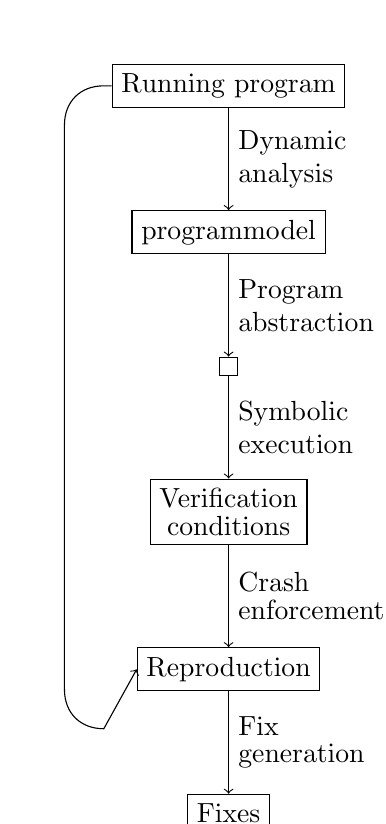
\begin{tikzpicture}
        [block/.style = {rectangle,draw,fill=white},
          node distance = 1.3]
        \node [block] (dynamic) {Running program};
        \node [block,below = of dynamic] (model) {\Gls{programmodel}};
        \node [block,below = of model] (statemachines) {\STateMachines};
        \node [block,below = of statemachines] (candidates) {\shortstack{Verification\\conditions}};
        \node [block,below = of candidates] (repro) {Reproduction};
        \node [block, below = of repro] (fix) {Fixes};
        \draw [->] (dynamic) to node [right] {\shortstack[l]{Dynamic\\analysis}} (model);
        \draw [->] (model) to node [right] {\shortstack[l]{Program\\abstraction}} (statemachines);
        \draw [->] (statemachines) to node [right] {\shortstack[l]{Symbolic\\execution}} (candidates);
        \draw [->] (candidates) to node [right] {\shortstack[l]{Crash\\enforcement}} (repro);
        \draw [->] (dynamic.west)
          -- ++(-.1,0)
          ..controls +(-0.3,0) and +(0, 0.3) .. ++(-0.5,-0.5)
          -- ++(0,-7.165)
          ..controls +(0,-0.3) and +(-0.3,0) .. ++( 0.5,-0.5)
          -- (repro.west);
        \draw [->] (repro) to node [right] {\shortstack[l]{Fix\\generation}} (fix);
      \end{tikzpicture}
    }
    \vspace{-4pt}
    \caption{System overview}
    \label{fig:basic_pipeline}
  \end{figgure}
  \vspace{-24pt}
\end{wrapfigure}
The basic approach is shown in \autoref{fig:basic_pipeline}.  The
process starts by observing the program's behaviour while operating
normally so as to build up a model of how it accesses memory.  This
model allows {\technique} to locate the parts of the program which are
most relevant to a particular concurrency error, and hence to build
\emph{\StateMachines} which more precisely model those areas.  These
     {\StateMachines} are then symbolically executed to determine
     whether running the modelled program fragments in parallel could
     lead to a concurrency error and, if so, to generate
     \glspl{verificationcondition} which precisely characterise the
     requirements for them to do so.  These
     \glspl{verificationcondition} are in turn used to construct
     co-programs which, when loaded into the running program, gently
     shepherd it towards these hypothesised bugs, allowing
     {\technique} to identify and discard any false positives with
     minimal manual intervention.  Any \glspl{verificationcondition}
     which survive this winnowing are then converted into binary
     patches which, when applied to the program, completely eliminate
     the bug.

All of these analyses and transformations are performed on the
program's machine code, with minimal (or in many non-trivial cases,
no) higher-level knowledge of the program's structure or environment.
This is in contrast to many previous systems, such as
Kivati~\cite{Chew2010} or AFix~\cite{Jin2011}, which operated on
either LLVM bitcode or the program's original source.  As such,
{\technique} can be applied to a wider class of programs, as it makes
no assumptions about the tools used to construct the program, and can
model the program's concurrency behaviour more accurately, as this
often depends on details of compiler optimisations which are visible
in machine code but not at higher levels.  On the other hand, the need
to infer information which other tools receive as input gives
{\technique} much higher computational cost, and this can limit its
applicability to more complicated bugs.  {\Technique} takes the
extreme position of attempting to analyse concurrency errors with
minimal support from the program, its environment, or its developers,
in some cases sacrificing practicality to do so.  As such, while it
can, as I demonstrate in the evaluation, often be usefully applied to
large software systems, such as MySQL or Thunderbird, it is perhaps
better thought of as an exploration of what can be achieved in an
unusually hostile analysis environment, and hence of the precise
trade-offs made when an analysis depends on richer input information,
rather than as a practical program maintenance technique in its own
right\editorial{That really isn't what I want to be saying.}.

\section{Contributions}

This dissertation makes several contributions:
\begin{itemize}
\item
  Suggest a novel method of finding and characterising
  concurrency-related bugs given only a binary program and some way of
  running it.
\item
  Describe how these characterisations can be used to automatically
  fix the bug or to make it more easily reproducible.
\item
  Evaluate the effectiveness and costs of these techniques with
  respect to a number of real and artificial test programs.
\end{itemize}
I give a detailed description of {\technique} and some results
obtained using \implementation, my prototype implementation.  These
include details of the fixes generated for a selection of bugs, both
artificial ones and some from real programs (including two which were
unknown to me before writing the tool), along with a demonstration
that the analysis scales to realistically large programs with
acceptable computational cost.  I also show that the fixes generated
typically have sufficiently low overhead to be useful in practice.

\section{Type of bug considered}
\label{sect:types_of_bugs}

{\Technique} considers only a subset of concurrency bugs: those where
one thread, referred to as the \gls{crashingthread}, is reading from a
shared data structure while another thread, the
\gls{interferingthread}, simultaneously modifies it, and these
concurrent updates cause the crashing thread to crash quickly.  In a
little more detail:
\begin{itemize}
\item The threads must be operating on a data structure located
  somewhere in shared memory.  This structure does not need to be in
  contiguous memory, and does not need to correspond to any
  higher-level concept of a data structure such as a C++
  \texttt{class} or \texttt{struct}, but it does need to be in
  process-accessible memory.  Structures on the filesystem, for
  instance, are not considered.
\item The \gls{crashingthread} must crash in a detectable way.  The
  simplest case is a hardware-detected fault such as referencing bad
  memory or dividing by zero, but more complex types of fault could
  also be supported, if a suitable detector can be implemented.
  {\Implementation} includes detectors for hardware-detected faults,
  assertion failures, and some types of double-free error.
\item The crash must be caused by the concurrent updates.  There must
  be some regions of the crashing and interfering threads such that
  running those regions in parallel can crash but running them
  atomically, in either order, will not.
\item The crashing thread must crash ``quickly''.  {\Technique} uses a
  finite \gls{analysiswindow} \gls{alpha} and will only consider
  reordering concurrent operations which occur at most \gls{alpha}
  instructions before the crash.  Bugs which require knowledge of the
  program behaviour beyond that window cannot be analysed.
  \gls{alpha} can, in principle, be arbitrarily large, but
  computational constraints mean that in practice it will be limited
  to a few dozen to a few hundred instructions, depending on the
  program to be analysed and how much information about the bug is
  available before analysis starts.
\end{itemize}
I refer to bugs which satisfy these constraints as \glslink{simple
  atomicity violation}{Simple Atomicity Violations}, or SAVs.  This
clearly does not include every possible type of concurrent bug (it
does not, for instance, include any but the most trivial deadlock
bugs, and complicated memory corruption bugs are difficult to handle),
but does include some interesting ones.

\begin{sanefig}
{\hfill}
\begin{tabular}{p{8cm}l}
Crashing thread:\hfill         & Interfering thread: \\
\\
1: Load $t_0$ from loc1        & 6: Load $t_3$ from loc1 \\
2: Store $t_0$ to loc2         & 7: Store $t_3$ to loc2 \\
\textit{Complicated local computation} & 8: Store $t_3 + 1$ to loc2 \\
3: Load $t_1$ from loc1        & \\
4: Load $t_2$ from loc2        & \\
5: Crash if $t_1 = t_2$ & \\
\end{tabular}
{\hfill}
\caption{An order violation bug. The complicated local computation
  does not modify loc1 or loc2.}
\label{fig:mandatory_concurrency1}
\end{sanefig}

\begin{sanefig}
\begin{centering}
\hfill
\begin{tabular}{p{8cm}l}
Crashing thread:          & Interfering thread: \\
\\
1: Load $t_0$ from loc1        & 6: Load $t_3$ from loc1 \\
2: Store $t_0+1$ to loc2       & 7: Store $t_3$ to loc2 \\
\textit{Complicated local computation} & 8: Store $t_3 + 1$ to loc2 \\
3: Load $t_1$ from loc1        & \\
4: Load $t_2$ from loc2        & \\
5: Crash if $t_1 = t_2$ & \\
\end{tabular}
\hfill
\end{centering}
\caption{Partial fix for the bug in
  \autoref{fig:mandatory_concurrency1}.}
\label{fig:mandatory_concurrency2}
\end{sanefig}

\subsection{Order-violation bugs}
The class of bugs described above does not include order violation
bugs, and so {\technique} will never report any.  Order violation bugs
in the program can, however, still sometimes affect the results.
Consider, for instance, the threads shown in
\autoref{fig:mandatory_concurrency1}.  These threads have an order
violation bug, in that the thread on the left will crash if it gets
from statement 2 to statement 3 before the thread on the right
executes.  Running the left-hand thread in isolation always leads to a
crash and so, within the definition used by {\technique}, this program
does not have a concurrency bug and no bug will be discovered,
reproduced, or fixed.

Suppose now that the ordering violation bug is fixed as shown in
\autoref{fig:mandatory_concurrency2}.  This program is ``more
correct'' than the previous one, in the sense that any instruction
interleaving which causes the new program to crash will also crash the
old one and some which crash the old will not crash the new, but
{\technique} \emph{will} report a potential bug in the new program.
Running the two new threads atomically, in either order, will never
crash, but interleaving them might (consider, for instance, the order
1, 2, 6, 7, 3, 4, 5).  The ordering violation bug effectively hid an
atomicity violation one, preventing {\technique} from finding either.

This non-monotonicity is an undesirable property for {\technique} to
have.  In practice, though, it is unlikely to be a serious problem.
Concurrency bugs in real programs tend to be at least moderately
difficult to reproduce, as easily reproduced bugs are generally fixed
quickly.  For this kind of bug, that implies that the local
computation must take time at least on the same order as operating
system scheduling effects, which usually range from a few tens of
microseconds to a few milliseconds.  On a modern process, that is
sufficient time to execute thousands to hundreds of thousands of
instructions, vastly exceeding {\technique}'s \gls{analysiswindow},
and so {\technique} is highly unlikely to capture an ordering
violation bug in the same window as an atomicity violation one.  If
two bugs are analysed in different windows then neither can hide the
other, and so there is little risk of an ordering violation disguising
an atomicity violation.

\subsection{Model of program execution}

In addition to restricting the class of bugs, {\technique} also
restricts the execution environment by assuming a strongly-ordered
memory model in which memory accesses are seen by all processors in
the order in which they appear in the program.  This is a reasonable
approximation for the widely-used x86 architecture, as that platform
rarely reorders memory accesses issued by a single
processor~\cite[Section 8.2]{Intel2009}.  Architectures with a weaker
memory ordering, such as Alpha~\cite[Section 5.6]{FFFCompaq2002} or
ARM~\cite[Section 5.3.4]{FFFARM2007}, would require more involved
processing to correctly capture the more complicated concurrency
semantics.

\section{Model of program modification}
\label{sect:intro:theory_of_fixing}

{\Technique} relies on being able to modify a program's behaviour in
order to reproduce and then to fix bugs, and aims to do so soundly, in
the sense that it should never introduce additional bugs.  This is not
entirely well-defined without access to a formal specification of the
program's desired behaviour.  It might be, for instance, that the
program is designed to investigate the possible ways in which a
particular processor can interleave memory accesses, and to report its
results by either exiting normally or crashing with an unhandled page
fault.  There is no general way for an automated tool to distinguish
such a program from one which is intended to always exit normally but
occasionally crashes due to an accidental race condition.  Any fix for
the latter would break the former.

{\Technique} defines a safe modification to a program to be one which
is equivalent to running it on a computer where some operations run
more slowly.  Equivalently, it will only ever introduce new bugs into
programs which depend on the relative timing of some operations.  This
is a reasonably conservative definition, in the sense that it allows
{\technique} to be applied to a reasonably broad variety of software,
but it is not quite universal.  In particular, {\technique} fixes and
\glspl{bugenforcer} can sometimes cause real-time programs to miss
their deadlines.  This is an inevitable risk when modifying a
program's scheduling without a precise specification of its deadline
structure, and, since {\technique} lacks such a specification, this is
the strongest safety property which can be hoped for.

\section{Graph generating grammars}
\label{sect:intro:graph_grammar}

\begin{sanefig}
  {\hfill}
  \tikzstyle{graphNT}+=[text width=1cm,fill=white]
  \begin{tabular}{lcclccrcc}
    \graphNT{$n$} & $\Rightarrow$ & \raisebox{-6mm}{\begin{tikzpicture}
        \node (n) {A};
        \node (nn) [style=graphNT, below=.5 of n] {$3n+1$};
        \draw[->] (n) -- (nn);
      \end{tikzpicture}} & \production{1} & \hspace{1cm} &
    \graphNT{2} & $\Rightarrow$ & \raisebox{-6mm}{
      \begin{tikzpicture}
        \node (2) {C};
        \node (1) [style = graphNT, below = .5 of 2] {1};
        \draw[->] (2) -- (1);
      \end{tikzpicture}
    } & \production{3} \\
    \graphNT{$m$} & $\Rightarrow$ & \raisebox{-6mm}{\begin{tikzpicture}
        \node (m) {B};
        \node (mm) [style=graphNT, below left =.5 of m] {$\frac{m}{2}$};
        \node (mmm) [style=graphNT, below right = .5 of m] {$\frac{m}{2} - 2$};
        \draw[->] (m) -- (mm);
        \draw[->] (m) -- (mmm);
    \end{tikzpicture}} & \production{2} & &
    \graphNT{4} & $\Rightarrow$ & \raisebox{-6mm}{
      \begin{tikzpicture}
        \node (4) {D};
        \node (2) [style=graphNT, below = .5 of 4] {2};
        \draw[->] (4) -- (2);
      \end{tikzpicture}
    } & \production{4} \\
  \end{tabular}
  {\hfill}
  \caption{Productions for the example graph generating grammar.  The
    terminals of this grammar are capital letters and the
    non-terminals are positive integers in boxes. $n$ matches odd
    integers and $m$ matches even integers other than two and four.
    Circled numbers are labels used to refer to the productions in the
    text.}
  \label{fig:intro:graph_grammar}
\end{sanefig}
\begin{sanefig}
  \newcommand{\arrowwidth}{0.03}
  \newcommand{\arrowhead}{0.05}
  \newcommand{\arrowlength}{0.8}
  \newcommand{\arrowdecoration}{}
  \newcommand{\labelledarrow}[1]{
    \hspace{-3.5mm}
    \begin{tikzpicture}
      \draw [\arrowdecoration] (0,-\arrowwidth) -- ++(\arrowlength,0);
      \draw [\arrowdecoration] (0,\arrowwidth) -- ++(\arrowlength,0);
      \draw [\arrowdecoration] (\arrowlength - \arrowhead + 0.01, 0 - \arrowwidth - \arrowhead) -- (\arrowlength + \arrowhead / 3 + \arrowwidth / 3, 0) -- (\arrowlength - \arrowhead + 0.01, \arrowwidth + \arrowhead);
      \node at (\arrowlength / 2,0) [above] {#1};
    \end{tikzpicture}\hspace{-3.5mm}
  }
  \tikzstyle{graphNT}+=[text width=1em, fill=white]
  \centerline{
  \begin{tikzpicture}[baseline=(r.base)]
    \node [style=graphNT] (r) {3};
  \end{tikzpicture}
  \labelledarrow{\production{1}}
  \begin{tikzpicture}[baseline=(r.base)]
    \node (r) {A\!\!};
    \node [left=-8pt of r] (r3) {\graphNT{3}:};
    \node [below = of r, style=graphNT] (s) {10};
    \draw[->] (r) -- (s);
  \end{tikzpicture}
  \labelledarrow{\production{2}}
  \begin{tikzpicture}[baseline=(r.base)]
    \node (r) {A\!\!};
    \node [left=-8pt of r] (r3) {\graphNT{3}:};
    \node [below=.57 of r] (s) {B\!\!};
    \node [left=-8pt of s] (r10) {\graphNT{10}:};
    \node [below=of s, style=graphNT] (t) {5};
    \draw[->] (r) -- (s);
    \draw[->] (s) -- (t);
    \draw[->] (s.east) .. controls +(.2,0) and +(0,-.2) .. ++(.33,.3) -- ++(0,0.55) .. controls +(0,.2) and +(.2,0) .. ++(-.3,.3) -- (r.east);
  \end{tikzpicture}
  \labelledarrow{\production{1}}
  \begin{tikzpicture}[baseline=(r.base)]
    \node (r) {A\!\!};
    \node [left=-8pt of r] (r3) {\graphNT{3}:};
    \node [below=.57 of r] (s) {B\!\!};
    \node [left=-8pt of s] (r10) {\graphNT{10}:};
    \node [below=.57 of s] (t) {A\!\!};
    \node [left=-8pt of t] (r10) {\graphNT{5}:};
    \node [below=of t,style=graphNT] (u) {16};
    \draw[->] (r) -- (s);
    \draw[->] (s) -- (t);
    \draw[->] (t) -- (u);
    \draw[->] (s.east) .. controls +(.2,0) and +(0,-.2) .. ++(.33,.3) -- ++(0,0.55) .. controls +(0,.2) and +(.2,0) .. ++(-.3,.3) -- (r.east);
  \end{tikzpicture}
  \labelledarrow{\production{2}}
  \begin{tikzpicture}[baseline=(r.base)]
    \node (r) {A\!\!};
    \node [left=-8pt of r] (r3) {\graphNT{3}:};
    \node [below=.57 of r] (s) {B\!\!};
    \node [left=-8pt of s] (r10) {\graphNT{10}:};
    \node [below=.57 of s] (t) {A\!\!};
    \node [left=-8pt of t] (r10) {\graphNT{5}:};
    \node [below=.57 of t] (u) {B\!\!};
    \node [left=-8pt of u] (r16) {\graphNT{16}:};
    \path (u.south) ++(-.7,-1) node [style=graphNT] (v) {8};
    \path (u.south) ++(.6,-1) node [style=graphNT] (w) {6};
    \draw[->] (r) -- (s);
    \draw[->] (s) -- (t);
    \draw[->] (t) -- (u);
    \draw[->] (u) -- (v);
    \draw[->] (u) -- (w);
    \draw[->] (s.east) .. controls +(.2,0) and +(0,-.2) .. ++(.33,.3) -- ++(0,0.55) .. controls +(0,.2) and +(.2,0) .. ++(-.3,.3) -- (r.east);
  \end{tikzpicture}
  \labelledarrow{\production{2}}
  \begin{tikzpicture}[baseline=(r.base)]
    \node (r) {A\!\!};
    \node [left=-8pt of r] (r3) {\graphNT{3}:};
    \node [below=.57 of r] (s) {B\!\!};
    \node [left=-8pt of s] (r10) {\graphNT{10}:};
    \node [below=.57 of s] (t) {A\!\!};
    \node [left=-8pt of t] (r10) {\graphNT{5}:};
    \node [below=.57 of t] (u) {B\!\!};
    \node [left=-8pt of u] (r16) {\graphNT{16}:};
    \path (u.south) ++(-.7,-.85) node [inner sep = 1.5 pt] (v) {B};
    \node [left=-7pt of v] (r8) {\graphNT{8}:};
    \path (v.south) ++(-.5,-1) node [style=graphNT] (x) {4};
    \path (v.south) ++(.5,-1) node [style=graphNT] (y) {2};
    \path (u.south) ++(.6,-1) node [style=graphNT] (w) {6};
    \draw[->] (r) -- (s);
    \draw[->] (s) -- (t);
    \draw[->] (t) -- (u);
    \draw[->] (u) -- (v);
    \draw[->] (u) -- (w);
    \draw[->] (v) -- (x);
    \draw[->] (v) -- (y);
    \draw[->] (s.east) .. controls +(.2,0) and +(0,-.2) .. ++(.33,.3) -- ++(0,0.55) .. controls +(0,.2) and +(.2,0) .. ++(-.3,.3) -- (r.east);
  \end{tikzpicture}
  }
  \centerline{
  \labelledarrow{$\cdots$}
  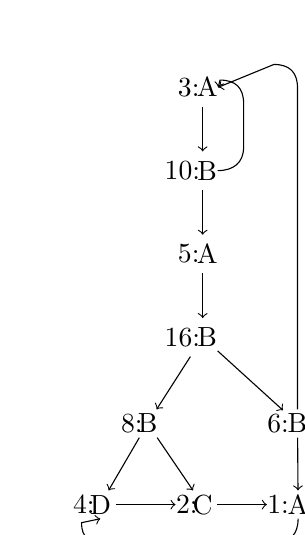
\begin{tikzpicture}[baseline=(r10.base)]
    \node (r) {A\!\!};
    \node [left=-8pt of r] (r3) {\graphNT{3}:};
    \node [below=.57 of r] (s) {B\!\!};
    \node [left=-8pt of s] (r10) {\graphNT{10}:};
    \node [below=.57 of s] (t) {A\!\!};
    \node [left=-8pt of t] (r10) {\graphNT{5}:};
    \node [below=.57 of t] (u) {B\!\!};
    \node [left=-8pt of u] (r16) {\graphNT{16}:};
    \path (u.south) ++(-.7,-.85) node [inner sep = 1.5 pt] (v) {B};
    \node [left=-7pt of v] (r8) {\graphNT{8}:};
    \path (v.south) ++(-.6,-.85) node [inner sep = 1.5pt] (x) {D};
    \node [left=-7pt of x] (r4) {\graphNT{4}:};
    \path (v.south) ++(.7,-.85) node [inner sep = 1.5pt] (y) {C};
    \node [left=-7pt of y] (r2) {\!\!\graphNT{2}:};
    \path (u.south) ++(.9,-.85) node (w) {\!\!\graphNT{6}:\!\!\!\!};
    \path (r2 -| w) node (z) {\!\!\graphNT{1}:\!\!\!\!};
    \node [right=1pt of z] [inner sep = 1.5pt] (z2) {A};
    \node [right=1pt of w] [inner sep = 1.5pt] (z3) {B};
    \draw[->] (r) -- (s);
    \draw[->] (s) -- (t);
    \draw[->] (t) -- (u);
    \draw[->] (u) -- (v);
    \draw[->] (u) -- (z3);
    \draw[->] (v) -- (x);
    \draw[->] (v) -- (y);
    \draw[->] (x) -- (r2);
    \draw[->] (y) -- (z);
    \draw[->] (z3) -- (z2);
    \draw[->] (s.east) .. controls +(.2,0) and +(0,-.2) .. ++(.33,.3) -- ++(0,0.55) .. controls +(0,.2) and +(.2,0) .. ++(-.3,.3) -- (r.east);
    \draw[->] (z2.south) .. controls +(0,-.2) and +(.2,0) .. ++(-.3,-.3) -- ++(-2.15,0) .. controls +(-.2,0) and +(0,-.2) .. ++(-.3,.25) -- (x.south);
    \draw[->] (z3.north) -- ++(0,4.08) .. controls +(0,.2) and +(.2,0) .. ++(-.3,.3) -- (r.east);
  \end{tikzpicture}
  \labelledarrow{}
  \begin{tikzpicture}[baseline=(r10.base)]
    \node (r) {\!\!A\!\!};
    \node [below=.57 of r] (s) {\!\!B\!\!};
    \node [below=.57 of s] (t) {\!\!A\!\!};
    \node [below=.57 of t] (u) {\!\!B\!\!};
    \path (u.south) ++(-.8,-.85) node [inner sep = 1.5 pt] (v) {B};
    \path (v.south) ++(-.55,-.85) node [inner sep = 1.5pt] (x) {D};
    \path (v.south) ++(.55,-.85) node [inner sep = 1.5pt] (y) {C};
    \path (u.south) ++(.8,-.85) node [inner sep = 1.5pt] (z3) {B};
    \path (y -| z3) node [inner sep = 1.5pt] (z2) {A};
    \draw[->] (r) -- (s);
    \draw[->] (s) -- (t);
    \draw[->] (t) -- (u);
    \draw[->] (u) -- (v);
    \draw[->] (u) -- (z3);
    \draw[->] (v) -- (x);
    \draw[->] (v) -- (y);
    \draw[->] (x) -- (y);
    \draw[->] (y) -- (z2);
    \draw[->] (z3) -- (z2);
    \draw[->] (s.east) .. controls +(.2,0) and +(0,-.2) .. ++(.33,.3) -- ++(0,0.55) .. controls +(0,.2) and +(.2,0) .. ++(-.3,.3) -- (r.east);
    \draw[->] (z2.south) .. controls +(0,-.2) and +(.2,0) .. ++(-.3,-.3) -- ++(-1.55,0) .. controls +(-.2,0) and +(0,-.2) .. ++(-.3,.25) -- (x.south);
    \draw[->] (z3.north) -- ++(0,4.08) .. controls +(0,.2) and +(.2,0) .. ++(-.3,.3) -- (r.east);
  \end{tikzpicture}
  }
  \caption[Expansion of a non-terminal using the productions in
    \autoref{fig:intro:graph_grammar}]{Expansion of the non-terminal
    \graphNT{$\mathrm{3}$} using the productions in
    \autoref{fig:intro:graph_grammar}.  Circled numbers above the
    arrows show which production was used at each step.}
  \label{fig:intro:graph_grammar:expansion}
\end{sanefig}

\noindent
Several of the algorithms in this dissertation are described in terms
of graph generating node-replacement grammars, and so I now give a
brief overview of this formalism using the example in
\autoref{fig:intro:graph_grammar}.  This figure shows a simple grammar
which produces directed graphs of (terminal) capital letters starting
from a single (non-terminal) integer.  The grammar works by matching a
pattern (on the left of the $\Rightarrow$) against some non-terminal
in the graph, possibly defining some match variables (in the example,
$n$ and $m$) in the process, generating a new fragment of graph (on
the right of the $\Rightarrow$), and replacing the original
non-terminal with the fragment.  This repeats until there are no more
non-terminals in the graph.  A non-terminal can only be generated at
most once; if a non-terminal is generated multiple times then it is
only added the first time and subsequent instances re-use the first
one.

\autoref{fig:intro:graph_grammar:expansion} shows how to apply this
grammar to the initial non-terminal \graphNT{3}.  The only production
that matches this initial graph is \production{1} with $n = 3$, which
generates a new terminal A with a single successor non-terminal
\graphNT{$3n+1$} = \graphNT{10}.  This non-terminal matches production
\production{2} with $m=10$, producing a terminal B and non-terminals
\graphNT{$\frac{m}{2}$}=\graphNT{5} and \graphNT{$\frac{m}{2}-2$} =
\graphNT{3}.  The \graphNT{3} non-terminal has already been generated
once, and so rather than adding a new node to the graph the grammar
adds an edge back to the previous one.  The grammar continues
expanding non-terminals in this way until none remain, producing the
graph at the bottom left of the figure.  The mapping from terminal
nodes to the non-terminals which generated them can then be forgotten,
producing the final graph at the bottom right of the figure.

\section{Structure of this dissertation}

This dissertation will, over the following chapters, present a
detailed description of how {\technique} works, starting with the
mechanism used to find and characterise bugs (\autoref{sect:derive})
and then moving on to describe how it first reproduces
(\autoref{sect:reproducing_bugs}) and then fixes
(\autoref{sect:fix_global_lock}) those bugs.  With the technique
itself described, I then give some experimental results obtained with
my prototype implementation {\implementation} (\autoref{chapter:eval})
and compare the technique to existing work in this area
(\autoref{chapter:related_work}).  Finally, I conclude and suggest
some possible avenues for future work (Chapters~\ref{sect:fw}
and~\ref{sect:concl}).


\chapter{Finding bugs}
\section{Finding candidate bugs}

The first phase of analysis is to locate all of the places in the program which might exhibit a bug of the desired class.

\subsection{Formal definition of the kind of bug which we look for}
\label{sect:finding_bugs:finding_candidate_bugs:formal_definition}
For the purposes of this section, we define a bug to be a tuple $(R, W, P)$ such that:

\begin{itemize}
\item[P valid] $P$ is a sequence of dynamic instructions which form a prefix of a possible execution of the program.
\item[R valid] $R$ is a sequence of dynamic instructions in a single thread such that $P \concatDynTraces R$, where $\concatDynTraces$ is simple concatenation, is a prefix of a possible execution of the program.
\item[W valid] Similarly, $W$ is a sequence of dynamic instructions in a single thread such that $P \concatDynTraces W$ is a prefix of a possible execution of the program.
\item[R atomic] $P \concatDynTraces R$ does not crash.
\item[W atomic] $P \concatDynTraces W \concatDynTraces R$ does not crash.
\item[W isolation] $W$ does not load from any locations which are stored to by $R$.
\item[Crash possible] $P \concatDynTraces (W \interleaveDynTraces R)$ can crash, where $\interleaveDynTraces$ is the interleaving of dynamic instruction traces.
\item[Concurrent] It is possible for the program to be in state S with one thread at the first instruction of $R$ while another thread is simultaneously at the first instruction of $W$.
\end{itemize}

We assume that programs execute an infinite sequence of no-op operations before the start of the program itself.

The intuition for this is that R is an operation which reads from some
shared structure and W is an operation which updates it, and the bugs
which we're looking for are those where inadequate synchronisation
causes the read operation to crash.  The R atomic and W atomic rules
ensure that we only need to consider concurrency-related bugs (if some
behaviour is possible when the machines are run atomically then it
clearly isn't a concurrency bug).  W isolation is a somewhat
unfortunate property, and restricts the set of bugs which we can
consider in an important way, but is necessary for the analysis to be
tractable~\needCite{}.

\subsubsection{Assumptions about the program}

Big ones:

\begin{itemize}
\item
  Only need to consider two threads at a time.  This is stronger than
  just assuming that each bug only involves two threads, because a
  third thread can sometimes make a race either possible or not
  possible, and that can lead to bug hiding as $N_r$ increases.
\item
  The no-mandatory-concurrency assumption.
\end{itemize}

\subsubsection{Effect of setting the $N_r$ and $N_w$}

The set of bugs detected by SLI depends on the size of the two
analysis windows, $N_r$ and $N_w$.  Setting these to two small a value
will of course lead to bugs being missed; more subtly, increasing the
size of the window can also sometimes lead to the set of bugs which is
reported shrinking.  This happens when the program depends on a
certain minimum level of concurrency in order to achieve correctness:
SLI assumes that the program does not crash if all of the instructions
in the analysis window are run atomically; if the program requires
some minimum level of interleaving this assumption can be violated for
some interesting executions, and enlarging the analysis window will
make the problem worse.

\begin{figure}
\begin{tabular}{ll}
Read thread:         & Write thread: \\
\\
Load $t$ from loc1   & Load $t'''$ from loc1 \\
Store $t$ to loc2    & Store $t'''$ to loc2 \\
Load $t'$ from loc1  & Store $t''' + 1$ to loc2 \\
Load $t''$ from loc2 & \\
Crash if $t' == t''$ & \\
\end{tabular}
\label{fig:mandatory_concurrency1}
\caption{Example of threads with mandatory concurrency.}
\end{figure}

\begin{figure}
\begin{tabular}{ll}
Read thread:          & Write thread: \\
\\
Load $t'$ from loc1   & Load $t'''$ from loc1 \\
Load $t''$ from loc2  & Store $t'''$ to loc2 \\
Crash if $t' == t''$  & Store $t''' + 1$ to loc2
\end{tabular}
\label{fig:mandatory_concurrency2}
\caption{Truncation of the example in figure~\ref{fig:mandatory_concurrency1}.}
\end{figure}

As a concrete example, consider the threads show in
figure~\ref{fig:mandatory_concurrency1}.  Running the read thread
atomically is guaranteed to crash, from any starting state, and so
there will be no valid bug tuples based on the complete definition of
these threads.  On the other hand, if the read thread is truncated as
shown in figure~\ref{fig:mandatory_concurrency2} then there may be
such a tuple:

\begin{itemize}
\item The R atomic rule is satisfied provided that the initial value of loc1 is not equal to loc2.
\item The W atomic rule is satisfied by any initial state.
\item The concurrent rule is satisfied by this crashing interleaving:
  \begin{itemize}
  \item Load $t'$ from loc1
  \item Load $t'''$ from loc1
  \item Store $t'''$ to loc2
  \item Load $t''$ from loc2
  \item Crash if $t' == t''$
  \end{itemize}
\end{itemize}

In this particular case, the crashing execution is far more likely
than the non-crashing one even when the threads are being run in
parallel and so it is highly unlikely that this precise behaviour
would be found in a real program.  On the other hand, if there were a
large amount of code between the final two load operations in the
final thread then it might make the surviving interleaving unlikely.
This is not generally an issue for SLI, as introducing enough extra
instructions to ensure that behaviour would generally push the first
load out of the analysis window so that SLI never sees the confusing
behaviour.  This means that, for most practical purposes, the set of
bugs found by increases monotonically with the size of the analysis
window, which in turn means that a very simple heuristic suffices for
setting the size of the window: use the largest window which allows
the analysis to complete in an acceptable amount of time.

\todo{It'd be nice to have some evidence of that.}

A more powerful analysis framework might be able to increase the
window size sufficiently that the first part of the read thread would
not ``fall out''.  Even in that case, the monotonicity property would
probably still hold for most realistic programs.  The fundamental
problem here is one of mandatory concurrency: in the larger program,
running the read thread in isolation is guaranteed to crash, but it
can be ``rescued'' by being interleaved with the write thread.  The
bug here is caused by insufficient concurrency, but SLI is only
capable of handling bugs caused by excessive concurrency.
Excess-concurrency bugs are far more common than
insufficient-concurrency bugs, for several reasons:

\begin{itemize}
\item
  An insufficient-concurrency bug indicates that the programmer got
  the sequential case wrong but the concurrent case correct.  The
  concurrent case is usually far more difficult to design and reason
  about than the sequential one, and so this is an unusual
  outcome\needCite{}.
\item
  The sequential case generally receives more testing than the
  concurrent one, simply as an artifact of the way most test cases are
  constructed\needCite{}.
\item
  For most programs, there are far more concurrent executions than
  sequential ones, and so it is more likely that there are errors on
  an untested concurrent path than that there are errors on an
  untested sequential one.
\end{itemize}

SLI therefore completely ignores these insufficient-concurrency bugs.

\todo{Mention something about finding a bunch of
  insufficient-concurrency bugs related to malloc() failure?}

\begin{figure}
Illustration of a bug tuple.  We have a prefix P, write section W, and read section R.
\label{fig:mandatory_concurrency3}
\end{figure}

I now show that insufficient-concurrency bugs are the only case in
which the monotonicity property might be violated.  To see this,
consider execution shown in figure~\ref{fig:mandatory_concurrency3}.
Suppose that this execution does not generate a bug tuple.  Then
moving an instruction from $R$ or $W$ into $P$ also cannot generate a
bug tuple, and so by induction no smaller analysis windows can
generate bug tuples.

From the fact that larger windows do not generate bug tuples, we know
that:

\begin{itemize}
\item $P \concatDynTraces R \not= \survive$, from the R atomic rule, or
\item $P \concatDynTraces W \concatDynTraces R \not= \survive$, from the W atomic rule, or
\item $\crash \notin P \concatDynTraces (R \interleaveDynTraces W)$, from the concurrent rule.
\end{itemize}

Define $W = w \concatDynTraces W'$ and $R = r \concatDynTraces R'$, so
that $w$ is the first instruction of $W$ and $W'$ all the others, and
likewise for $r$, $R$, and $R'$.  Shrinking the analysis window then
corresponds to replacing $R$ with $R'$ and $P$ with $P
\concatDynTraces r$, or replacing $W$ with $W'$ and $P$ with $P
\concatDynTraces w$.  We therefore generate a bug tuple with the
reduced window if:

\begin{align*}
( & (P \concatDynTraces w \concatDynTraces R & = & \survive) & \wedge \\
  & (P \concatDynTraces W \concatDynTraces R & = & \survive) & \wedge \\
  & ((P \concatDynTraces w \concatDynTraces (R \interleaveDynTraces W')) & \ni & \crash)) & \vee \\
( & (P \concatDynTraces R & = & \survive) & \wedge \\
  & (P \concatDynTraces r \concatDynTraces W \concatDynTraces R' & = & \survive) & \wedge \\
  & ((P \concatDynTraces r \concatDynTraces (R' \interleaveDynTraces W)) & \ni & \crash))
\end{align*}

Combining those together, we find that reducing the analysis window can introduce a new bug if:

\begin{align*}
( & (P \concatDynTraces R & \not= & \survive) & \wedge \\
  & (P \concatDynTraces W \concatDynTraces R & \not= & \survive) & \wedge \\
  & ((P \concatDynTraces (R \interleaveDynTraces W)) & \not{}\ni & \crash)) & \vee \\
( & (P \concatDynTraces w \concatDynTraces R & = & \survive) & \wedge \\
  & (P \concatDynTraces W \concatDynTraces R & = & \survive) & \wedge \\
  & ((P \concatDynTraces w \concatDynTraces (R \interleaveDynTraces W')) & \ni & \crash)) & \vee \\
( & (P \concatDynTraces R & = & \survive) & \wedge \\
  & (P \concatDynTraces r \concatDynTraces W \concatDynTraces R' & = & \survive) & \wedge \\
  & ((P \concatDynTraces r \concatDynTraces (R' \interleaveDynTraces W)) & \ni & \crash))
\end{align*}

Simple boolean algebra, plus the obvious rule that $P \concatDynTraces (R \interleaveDynTraces W) = (P \concatDynTraces r \concatDynTraces (R' \interleaveDynTraces W) ) \cup (P \concatDynTraces w \concatDynTraces (R \interleaveDynTraces W') ) $, reduces that to this:

\begin{align*}
( & (P \concatDynTraces r \concatDynTraces R' & = & \crash) & \wedge \\
  & (P \concatDynTraces w \concatDynTraces r \concatDynTraces R' & = & \survive) & \wedge \\
  & (P \concatDynTraces w \concatDynTraces W' \concatDynTraces r \concatDynTraces R' & = & \survive) & \wedge \\
  & ((P \concatDynTraces w \concatDynTraces (W' \interleaveDynTraces R)) & \ni & \crash)) & \vee \\
( & (P \concatDynTraces r \concatDynTraces R' & = & \survive) & \wedge \\
  & (P \concatDynTraces w \concatDynTraces W' \concatDynTraces r \concatDynTraces R' & = & \crash) & \wedge \\
  & (P \concatDynTraces w \concatDynTraces r \concatDynTraces R' & = & \survive) & \wedge \\
  & (P \concatDynTraces r \concatDynTraces w \concatDynTraces W' \concatDynTraces R' & = & \survive) & \wedge \\
  & ((P \concatDynTraces r \concatDynTraces (W \interleaveDynTraces R')) & \ni & \crash))
\end{align*}

Consider the first clause of the disjunction first, and in particular consider these two terms:

\begin{align*}
 & (P \concatDynTraces r \concatDynTraces R' & = & \crash) & \wedge \\
 & (P \concatDynTraces w \concatDynTraces r \concatDynTraces R' & = & \survive)
\end{align*}

The definition of crash used in SLI is that the final instruction of $R'$ crashes, and so adding further instructions after that point cannot possible change the result.
Those terms are therefore equivalent to these:

\begin{align*}
 & (P \concatDynTraces r \concatDynTraces R' \concatDynTraces w \concatDynTraces W' & = & \crash) & \wedge \\
 & (P \concatDynTraces w \concatDynTraces r \concatDynTraces R' \concatDynTraces W' & = & \survive)
\end{align*}

In other words, $R$ is doomed when run in isolation, but running it in parallel with $W$ can save it.
That is precisely the definition of mandatory concurrency used above.

Consider the second clause now.
That contains these two terms:

\begin{align*}
  & (P \concatDynTraces w \concatDynTraces W' \concatDynTraces r \concatDynTraces R' & = & \crash) & \wedge \\
  & (P \concatDynTraces r \concatDynTraces w \concatDynTraces W' \concatDynTraces R' & = & \survive)
\end{align*}

This is even more clear: running $W$ and then $R$ atomically leads to a crash, but allowing $W$ to interrupt $R$ saves the execution.
Once again, this clause is only satisfiable in the presence of mandatory concurrency.

Therefore, it is only possible for shrinking the analysis window to reveal more bugs in the presence of mandatory concurrency, and, conversely, when the program does not use mandatory concurrency, enlarging the analysis window cannot disguise bugs.
This monotonicity property is useful because it provides a simple rule for setting the size of the analysis window: use the largest such that the analysis completes in a reasonable amount of time.
There is no need for the user to carefully select a window size for their program, or to try multiple window sizes in order to reveal additional bugs.

\label{sect:monotonicity}

\todo{This proof feels quite circular and unconvincing.  May need more thought here.}

\subsection{Crash summaries}

This analysis produces a series of crash summaries.
Each summary represents a (possibly infinite) set of bug tuples has several components:

\begin{itemize}
\item The read \StateMachine, corresponding to the $R$ member of the bug tuple.
\item The write \StateMachine, corresponding to the $W$ member of the bug tuple.
\item The verification condition, a predicate on the program's state which corresponds to the $S$ member of the bug tuple.
\item An aliasing table, which says which memory-accessing instructions in the read and write \StateMachines might access the same area of memory.
\end{itemize}

A crash summary represents a bug tuple $(R, W, S)$ if the summary's read \StateMachine includes the dynamic instruction trace $R$, its write \StateMachine includes the dynamic instruction trace $W$, and the verification condition is true of $S$.
The set of summaries produced by the analysis is defined to be complete if every possible bug tuple is represented by at least one crash summary, and sound if the crash summaries only represent valid bug tuples.
The analysis presented here is, in that sense, complete, subject to some caveats discussed in later sections, but not sound.

\section{\STateMachines}

The \StateMachines themselves consist of three components:

\begin{itemize}
\item
  A slice of the program in a simple analysis language.  Programs in
  this language consist of a directed acyclic graph of analysis
  states.  The states fall into one of three classes: terminals, with
  no successors; side-effects, with a single successor; or choices,
  with two successors.  The side-effects can express obvious
  program-level effects such as accessing memory or setting a
  particular register, but also less-obvious ones such as register
  aliasing configurations or restrictions on the set of program states
  which must be considered by later analysis steps.  Similarly, the
  expression language used for the conditions in choice states or the
  addresses for memory accessing side-effects can refer to simple
  things like the values of processor registers or the initial
  contents of memory, and can also express queries about the program's
  control flow or the happens-before graph.
\item
  A fragment of the original program's control-flow graph, covering
  all of the instructions from which the \StateMachine was generated.
  This fragment is unrolled so that each dynamic instruction in the
  analysis window is represented by precisely on node in the
  CFG\editorial{I should really try to explain what that means in a
    bit more detail.}.  Functions are inlined.  This graph fragment
  will not always be completely weakly connected if, for instance, the
  \StateMachine represents activity in multiple concurrent threads.
\item
  A table mapping memory access identifiers to sets of nodes in the
  control flow graph. \todo{Screw it; these are a pain to describe and
    they're not all that important; drop them.}
\end{itemize}

\begin{figure}
  \begin{minipage}{50mm}
    \begin{subfloat}
      \begin{minipage}{50mm}
\begin{verbatim}
400694: mov    global_ptr,%rax
40069b: test   %rax,%rax
40069e: je     4006ad
4006a0: mov    global_ptr,%rax
4006a7: movl   $0x5,(%rax)
\end{verbatim}
      \end{minipage}
      \caption{Program code}
    \end{subfloat}
    \vspace{50pt}
    \begin{subfloat}
      \hspace{20mm}
      \begin{tikzpicture}
        \node (cfg6) at (0,2) [CfgInstr] {cfg6:400694};
        \node (cfg5) [CfgInstr, below=of cfg6] {cfg5:40069b};
        \node (cfg4) [CfgInstr, below=of cfg5] {cfg4:40069e};
        \node (cfg3) [CfgInstr, below=of cfg4] {cfg3:4006a0};
        \draw[->] (cfg6) -- (cfg5);
        \draw[->] (cfg5) -- (cfg4);
        \draw[->] (cfg4) -- (cfg3);
      \end{tikzpicture}
      \caption{Control-flow graph fragment}
    \end{subfloat}
  \end{minipage}
  \begin{subfloat}
    \begin{minipage}{30mm}
      \begin{tikzpicture}
        \node (l1) at (0,2) [stateSideEffect] {l1: LOAD tmp1 $\leftarrow$ global\_ptr AT cfg6 };
        \node (l2) [stateIf, below=of l1] {l2: if (0 == tmp1)};
        \node (l4) [stateSideEffect, below=of l2] {l4: LOAD tmp2 $\leftarrow$ global\_ptr AT cfg3 };
        \node (l3) [stateTerminal, right=of l4] {l3: survive};
        \node (l5) [stateIf, below=of l4] {l5: if (BadPtr(tmp2))};
        \node (l6) [stateTerminal, below=of l5] {l6: crash};
        \draw[->] (l1) -- (l2);
        \draw[->] (l2) -- node [above] { true } (l3);
        \draw[->] (l2) -- node [left] { false } (l4);
        \draw[->] (l4) -- (l5);
        \draw[->] (l5) -- node [below] { false } (l3);
        \draw[->] (l5) -- node [left] { true } (l6);
      \end{tikzpicture}
    \end{minipage}
    \caption{\STateMachine}
  \end{subfloat}
  \label{fig:intro:single_threaded_machine}
  \caption{A fragment of machine code, and the \StateMachine generated
    for a bug which leads to a crash at 4006a7.}
\end{figure}

Figure~\ref{fig:intro:single_threaded_machine} shows an example of a
simple single-threaded \StateMachine\footnote{This is the read-side of
  the simple\_toctou test in \S\ref{sect:eval:art:simple_toctou}.}.
It illustrates a simple time-of-check, time-of-use race: the program
loads from \verb|global_ptr| twice in quick succession, validating the
result of the first and using the result of the second.  The
translation to a \StateMachine is hopefully reasonably clear: the
control-flow graph covers on the left all of the relevant instructions
and the flow chart on the right expresses the relevant part of their
behaviour.  It is trivial to read off from these diagrams that the
program might crash if some other thread modifies \verb|global_ptr| in
between the two loads and will otherwise survive.

\begin{figure}
  \begin{minipage}{50mm}
    \begin{subfloat}
      \begin{minipage}{50mm}
\begin{verbatim}
4008fb: movq   $0x0,global_ptr
\end{verbatim}
      \end{minipage}
      \caption{Program code}
    \end{subfloat}
    \vspace{50pt}
    \begin{subfloat}
      \hspace{20mm}
      \begin{tikzpicture}
        \node (cfg8) at (0,2) [CfgInstr] {cfg8:4008fb};
      \end{tikzpicture}
      \caption{Control-flow graph fragment}
    \end{subfloat}
  \end{minipage}
  \begin{subfloat}
    \begin{minipage}{30mm}
      \begin{tikzpicture}
        \node (l7) at (0,2) [stateSideEffect] {l7: STORE 0 $\rightarrow$ global\_ptr AT cfg8 };
      \end{tikzpicture}
    \end{minipage}
    \caption{\STateMachine}
  \end{subfloat}
  \label{fig:intro:single_threaded_machine_write}
  \caption{The other side of the race in figure~\ref{fig:intro:single_threaded_machine}.}
\end{figure}

\begin{figure}
  \begin{tikzpicture}
    \node (lA) [stateIf] { lA: if $cfg6:thread1 \happensBefore cfg7:thread2$ };
    \node (l1) [stateSideEffect, below left = of lA] { l1: LOAD tmp1 $\leftarrow$ global\_ptr AT cfg6:thread1 };
    \node (l2) [stateIf, below = of l1] { l2: if (0 == tmp1) };
    \node (lD) [stateTerminal, below left = of l2] { lD: survive};
    \node (lC) [stateIf, below right = of l2] {lC:  if $cfg3:thread1 \happensBefore cfg7:thread2$ };
    \node (lE) [stateSideEffect, below left = of lC] {lE: Assert $global\_ptr = global\_ptr$ };
    \node (l7a) [stateSideEffect, below = of lE] {l7a: STORE 0 $\rightarrow$ global\_ptr AT cfg8:thread2 };
    \node (l4a) [stateSideEffect, below = of l7a] {l4a: LOAD tmp2 $\leftarrow$ global\_ptr AT cfg3:thread1 };
    \node (l5a) [stateIf, below = of l4a] { l5a: if $BadPtr(tmp2)$ };
    \node (lG) [stateTerminal, below = of l5a] { lG: crash };
    \node (l4b) [stateSideEffect, below right = of lC] {l4b: LOAD tmp3 $\leftarrow$ global\_ptr AT cfg3:thread1 };
    \node (l5b) [stateIf, below = of l4b] { l5: if $BadPtr(tmp3)$ };
    \node (lF) [stateTerminal, below right = of l5b] { lF: unreached };
    \node (lB) [stateSideEffect, below right = of lA] { lB: Assert $global\_ptr = global\_ptr$ };
    \node (l7b) [stateSideEffect, below = of lB] { l7b: STORE 0 $\rightarrow$ global\_ptr AT cfg8:thread2 };
    \draw [->] (lA) -- (l1);
    \draw [->] (lA) -- (lB);
    \draw [->] (l1) -- (l2);
    \draw [->] (l2) -- (lD);
    \draw [->] (lC) -- (lE);
    \draw [->] (lC) -- (l4b);
    \draw [->] (lE) -- (l7a);
    \draw [->] (l7a) -- (l4a);
    \draw [->] (l4a) -- (l5a);
    \draw [->] (l5a) -- (lD);
    \draw [->] (l5a) -- (lG);
    \draw [->] (l4b) -- (l5b);
    \draw [->] (l5b) -- (lD);
    \draw [->] (l5b) -- (lF);
    \draw [->] (lB) -- (l7a);
    \draw [->] (l7a) -- (lF);
  \end{tikzpicture}
  \label{fig:intro:cross_thread}
  \caption{Cross-product of the \StateMachine shown in
    figures~\ref{fig:intro:single_threaded_machine} and
    \ref{fig:intro:single_threaded_machine_write}.}
\end{figure}

\begin{figure}
  \begin{tikzpicture}
    \node (lA) [stateSideEffect] {lA: Assert $0 \not= InitMemory(global\_ptr)$ and $cfg6:thread1 \happensBefore cfg7:thread2$};
    \node (lB) [stateIf, below = of lA] {lB: if $cfg3:thread1 \happensBefore cfg7:thread2$ };
    \node (lC) [stateTerminal, below left = of lB] {lC: survive};
    \node (lD) [stateTerminal, below right = of lB] {lD: crash};
    \draw [->] (lA) -- (lB);
    \draw [->] (lB) -- (lC);
    \draw [->] (lB) -- (lD);
  \end{tikzpicture}
  \label{fig:intro:cross_thread_opt}
  \caption{\STateMachine from figure~\ref{fig:intro:cross_thread}
    after \StateMachine simplification.}
\end{figure}

\STateMachines become somewhat more interesting when they capture the
results of multiple threads.  Figure~\ref{fig:intro:cross_thread}
shows an example of a cross-thread \StateMachine.  There are a couple
of interesting features here:

\begin{itemize}
\item Several new states have been created and existing ones
  duplicated.  In particular, some memory accesses have now been
  duplicated to multiple places in the \StateMachine
\item
  $\happensBefore$ expressions.  These allow the \StateMachine to
  query the program's happens-before graph.  $cfgA:threadB
  \happensBefore cfgC:threadD$ is true precisely when instruction $A$
  in thread $B$ happens before instruction $C$ in thread $D$.
  \todo{Whoops: the semantics of these depends on the memory access
    identifier indirection, so I guess I will have to describe that
    after all.}

  These expressions imply something important about the semantics of
  the \StateMachines.  In particular, a \StateMachine with a
  $\happensBefore$ edge cannot be interpreted as an approximation to a
  fragment of the program, but must instead be treated as a query over
  program executions.  \todo{Not convinced that's terribly clear, and
    it ought to be somewhere else.}
\item
  Assertion side-effects and the unreached state.  These are used to
  give later stages of the analysis hints about which paths through
  the combined \StateMachine are likely to be interesting.  Assertion
  side-effects specify indicate that if some condition is false then
  the \StateMachine is not worth analysing; later analysis phases make
  heavy use of these hints.  Likewise, any path which reaches an
  unreached state is not considered to be uninteresting.  These two
  mechanisms are of precisely equivalent power; SLI uses one or the
  other depending on which is more convenient at the time.
\item
  Paths in which either the store or load machine end without the
  other starting will end in an unreached state, so they will not be
  considered by the later analysis phases.  While not apparent in this
  simple example, the algorithm used by SLI also uses partial-order
  reduction\needCite{} to further reduce the number of interleavings
  to be considered.
\end{itemize}

The \StateMachine shown in figure~\ref{fig:intro:cross_thread}
correctly captures the interaction of the two input \StateMachines but
is more complicated than it needs to be.  SLI therefore performs a few
simplifications on the \StateMachine, detailed later, before passing
the \StateMachine to the symbolic execution engine; the results are
shown in figure~\ref{fig:intro:cross_thread_opt}\footnote{Similar
  simplifications are also applied to the single-threaded
  \StateMachines, but those are uninteresting in this case.}.

\STateMachines have a couple of other features not shown in this
example:

\begin{itemize}
\item
  Control-flow expressions.  Much as \StateMachines can query the
  happens-before graph of a program using $\happensBefore$
  expressions, they can also query the control flow within a given
  thread using $Entry$ and $ControlFlow$ expressions.  An
  $Entry(threadA:cfgB)$ expression is true if thread $A$ entered the
  CFG at CFG node $cfgB$, while $ControlFlow(threadA:cfgB->cfgC)$ is
  true if thread $A$ transitions from CFG node $B$ to node $C$.  Note
  that the value of $ControlFlow$ expression does not depend on where
  in the \StateMachine it is evaluated: the control flow within a
  \StateMachine is (conceptually) independent of that of the original
  program.
\item
  Static analysis side effects.  These are used to import the results
  of the initial whole-program static analysis into the \StateMachine.
  The most important of these is the Alias side-effect, which gives a
  points-to set of a given \StateMachine-level variable.  These
  points-to sets are expressed over stack frames, plus a flag saying
  whether the variable might point at a non-stack location.
\item
  $\Phi$ side-effects.  These are described later when discussing the
  SSA form used; they have a somewhat different semantic from the
  $\Phi$ nodes used in optimising compilers.
\item
  Start and end atomic side-effects.  These indicate that a given
  fragment of the \StateMachine should execute atomically, and hence
  restrict the cross-product \StateMachine.  They are used both to
  represent instructions with the \verb|LOCK| prefix (which execute
  atomically) and some library-level functions such as
  \verb|pthread_mutex_lock|\editorial{Should probably have a forwards
    ref to discussion of handling library functions.}.
\end{itemize}

%% They are also similar to the intermediate forms used by model
%% checkers such as SAL\editorial{Cite Park 2000; the Stanford Java
%% checker.}\editorial{Cite JPF and their arguments for not using
%% standard MC intermediate forms; they all apply here as well, and it
%% saves me having to argue it myself.}\editorial{Need to come up with
%% an argument for not just using SAL.}.  The key difference here is
%% less the nature of the intermediate form and more the way in which
%% it is used: SLI \StateMachines only model the part of a program
%% which might conceivably be relevant to some (real or hypothesised)
%% bug, whereas a model checker's intermediate form will usually
%% represent at least some aspect of the entire program component
%% which is to be analysed\editorial{Clumsy.  What I'm trying to say
%% here is that we slice on a different axis: model checkers build up
%% a model of the entire program which is relevant to the predicate
%% which they're checking, whereas SLI builds up a series of models
%% each of which is constrained on both the property (implicit) and
%% the place which we think might have a bug.  Also, describing it as
%% the key difference is kind of misleading: it's the key difference
%% here, but not really the most important one, which is what we use
%% the results for.}.

\subsection{Building read-side \StateMachines}

The aim of this phase of the algorithm is to find every fragment of the program which might act as the first ($R$) element of the bug tuple.
The simplest approach would be to simply enumerate every dynamic fragment containing $N_r$ instructions which ends in a memory-accessing instruction and convert each one independently into a \StateMachine.
While it would be effective, this would be extremely time consuming, especially for larger values of $N_r$, and would perform a large amount of redundant work.
SLI therefore uses a slightly more involved approach.

The core of the algorithm is to first select the final, crashing, instruction in the fragment, then to build up a static control-flow graph (CFG) containing every static instruction which might be part of the dynamic trace, unroll any loops in the graph until every path of length $N_r$ is represented, and then compile the resulting CFG into a \StateMachine.
This is repeated for every possible final instruction in the program.
The next few sections will describe this system in more detail.

\subsubsection{Building the static control-flow graph}
The first step of the algorithm, once a potentially-crashing instruction has been selected for investigation, is to build a static control-flow graph containing all of the instructions which might appear in the dynamic trace.
This is done by starting with a trivial CFG containing just the crashing instruction and then expanding it backwards, one instruction at a time, until every needed instruction has been discovered.

The simple case is that all of the needed instructions are contained within a single instruction.
In that case, the algorithm is as follows:

\begin{algorithmic}[1]
\STATE $depth \gets 0$
\STATE $pendingAtDepth \gets \queue{targetInstrAddress}$
\STATE $result \gets \map{}$
\WHILE{$depth < N_r$}
  \STATE $pendingAtNextDepth \gets \queue{}$
  \WHILE{$\neg{}empty(pendingAtDepth)$}
    \STATE $currentInstr \gets pop(pendingAtDepth)$
    \IF {$result \textrm{ has entry for } currentInstr$}
      \STATE \textbf{continue}
    \ENDIF
    \STATE $current \gets \text{decode instruction at } currentInstr$
    \STATE $\mapIndex{result}{currentInstr} \gets current$
    \STATE $predecessors \gets \text{predecessors of } currentInstr$
    \STATE Add $predecessors$ to $pendingAtNextDepth$
  \ENDWHILE
  \STATE $pendingAtDepth \gets pendingAtNextDepth$
  \STATE $depth \gets depth + 1$
\ENDWHILE
\end{algorithmic}

This algorithm builds, in $result$, a mapping from instruction addresses to decoded instructions, working backwards from the address of the potentially crashing instruction until every instruction which might be executed up to $N_r$ dynamic instructions before the target is present.

There is a slight subtlety on line 13, when determining the predecessors of a given instruction.
This is not always obvious, given only a binary program, for three reasons:

\begin{itemize}
\item
  The program might contain indirect branches.
  It is difficult to determine statically where these might branch to.
  A conservative approach would be to assume that they might branch anywhere, but this leads to unmanageably complex CFGs even for trivial programs.
  At the same time, ignoring them completely means that many important program paths will be missed.
\item
  The AMD64 instruction set includes variable-length instructions, and so there might be several overlapping instructions which all finish at the start of the instruction currently being investigated.
  In most programs, only one of these will ever be executed, and it is important to pick the right one.
\item
  It is not always trivial to locate all of the branch instructions in a program.
\end{itemize}

SLI solves this problem using a combination of static and dynamic analysis.
First, the dynamic analysis tracks the targets of all indirect branch and call instructions.
This makes the first problem trivial (assuming that the dynamic analysis is complete).
It also means that a simple static analysis can enumerate every instruction reachable from the program's entry point (which can itself be determined from the ELF binary's metadata), hence building up a complete CFG of the entire program.
That CFG then makes solving the second and third problems trivial.

\todo{Slight complication for async OS callbacks like signal handlers.}

\todo{There are two different CFGs here.  Should maybe do some alpha conversion to remove that ambiguity.}

\todo{Point out that the CFG can have multiple roots here.}

\subsubsection{Handling loops in the CFG}
\editorial{This is very similar to the way we handle loops in the
  write-side CFG, but more complicated and harder to explain.  That
  suggests that we should maybe explain the write-side algorithm
  first, except that the write-side CFG generation algorithm uses the
  read-side CFG as one of its inputs, which then makes that much
  harder to describe.}

There may be loops in the CFGs generated by this algorithm, but SLI requires that the \StateMachines be finite and acyclic.
These loops must therefore be eliminated in a way which is guaranteed to preserve all paths of length $N_r$.
The approach SLI takes is, in essence, to unroll the loops, duplicating instructions as necessary, until every path from a root of the CFG to the target instruction is either free from cycles or of length greater than $N_r$.

\begin{tikzpicture}
  [node distance=1 and 0.3]
  \begin{scope}
    \node (A) at (0,2) [CfgInstr] {A};
    \node (B) [CfgInstr] [below=of A] {B}; 
    \node (C) [CfgInstr] [below=of B] {C}; 
    \node (D) [CfgInstr] [below=of C] {D}; 
    \draw[->] (A) -- (B);
    \draw[->] (B) -- (C);
    \draw[->] (C) -- (D);
    \draw[->] (C.east) to [bend right=90] (B.east) node (edge1) [right] {};
    \begin{pgfonlayer}{bg}
      \node (box1) [fill=black!10,fit=(A) (B) (C) (D) (edge1)] {};
    \end{pgfonlayer}
  \end{scope}
  \begin{scope}[xshift=4cm]
    \node (A) at (0,2) [CfgInstr] {A};
    \node (B) [CfgInstr] [below=of A] {B}; 
    \node (C) [CfgInstr] [below=of B] {C}; 
    \node (D) [CfgInstr] [below=of C] {D};  
    \node (C') [CfgInstr] [right=of C] {C'};
    \draw[->] (A) -- (B);
    \draw[->] (B) -- (C);
    \draw[->] (C) -- (D);
    \draw[->] (B) to [bend right=10] (C');
    \draw[->] (C') to [bend right=10] (B);
    \begin{pgfonlayer}{bg}
      \node (box2) [fill=black!10,fit=(A) (B) (C) (D) (C')] {};
    \end{pgfonlayer}
  \end{scope}
  \begin{scope}[xshift=8cm]
    \node (A) at (0,2) [CfgInstr] {A};
    \node (B) [CfgInstr] [below=of A] {B};
    \node (B') [CfgInstr] [right=of B] {B'};
    \node (C) [CfgInstr] [below=of B] {C};
    \node (D) [CfgInstr] [below=of C] {D};
    \node (C') [CfgInstr] [right=of C] {C'};
    \draw[->] (A) -- (B);
    \draw[->] (B) -- (C);
    \draw[->] (C) -- (D);
    \draw[->] (C') -- (B);
    \draw[->] (A) -- (B');
    \draw[->] (B') to [bend right=10] (C');
    \draw[->] (C') to [bend right=10] (B');
    \begin{pgfonlayer}{bg}
      \node (box3) [fill=black!10,fit=(A) (B) (C) (D) (C') (B')] {};
    \end{pgfonlayer}
  \end{scope}
  \begin{scope}[xshift=12cm]
    \node (A) at (0,2) [CfgInstr] {A};
    \node (B) [CfgInstr] [below=of A] {B};
    \node (B') [CfgInstr] [right=of B] {B'};
    \node (C) [CfgInstr] [below=of B] {C};
    \node (C') [CfgInstr] [right=of C] {C'};
    \node (C'') [CfgInstr] [right=of C'] {C''};
    \node (D) [CfgInstr] [below=of C] {D};
    \draw[->] (A) -- (B);
    \draw[->] (B) -- (C);
    \draw[->] (C) -- (D);
    \draw[->] (C') -- (B);
    \draw[->] (A) -- (B');
    \draw[->] (B') -- (C');
    \draw[->] (C'') to [bend right=10] (B');
    \draw[->] (B') to [bend right=10] (C'');
    \begin{pgfonlayer}{bg}
      \node (box4) [fill=black!10,fit=(A) (B) (C) (D) (C') (B') (C'')] {};
    \end{pgfonlayer}
  \end{scope}
  \draw[->,thick] (box1) -- (box2) node [above,midway] {duplicate C};
  \draw[->,thick] (box2) -- (box3) node [above,midway] {duplicate B};
  \draw[->,thick] (box3) -- (box4) node [above,midway] {duplicate C'};
  \draw[->,thick] (box4) -- +(2.5,0) node [above,midway] {...};
\end{tikzpicture}

The diagram shows a CFG with four instructions, A, B, C, and D, and a loop between B and C.
This loop must be removed from the CFG whilst maintaining all paths which terminate at D and which contain $N_r$ instructions.
SLI does this by duplicating nodes in the CFG so as to unroll the loop and hence increase the distance between the loop and instruction D.
Consider the leftmost diagram first.
SLI will start at instruction D and perform a depth-first traversal backwards through the graph until it finds an edge which closes a cycle; in this case, that is the edge from C to B.
We will therefore try to break the cycle along this edge.
Note that we break on the back edge, C to B, rather than the forwards edge B to C.
To break the edge, SLI duplicates the instruction at the start of the edge and all of the edges to that instruction (in this case, duplicating C to form C' and the B to C edge to form a B to C' edge).
It then redirects the breaking edge to come from the new instruction (so the edge from C to B is replaced by an edge from C' to B).
All paths which were possible in the old graph will also be possible in the new one, if duplicated nodes are treated as semantically equivalent, and the loop is now one instruction further away from the target instruction D.

There is still a cycle in this graph, and so the process will repeat.
In this case, the first cycle encountered when performing depth-first traversal backwards from D is the B to C' edge, and so the loop will be broken on that edge by duplicating B to form B'.
As before, all of the incoming edges of the duplicated node are duplicated as well, so new edges are created from A to B' and from C' to B'.
The B to C' edge is then replaced with one from B' to C'.
Again, all paths through the graph are preserved and the cycle moved further away from D.

This algorithm can be iterated as many times as necessary until the cycle is at least $N_r$ instructions away from D.
At that point, every path of length $N_r$ traverses the cycle at most once, and so the cycle can be removed completely without changing the set of possible paths through the graph.

\begin{algorithmic}
  \WHILE {graph is not cycle-free}
     \STATE $edge \gets findEdgeToBeBroken(targetInstr, \{\})$
     \IF {$edge$ is at least $N_f$ instructions from target instruction}
        \STATE {Erase $edge$ from graph}
     \ELSE
        \STATE {$newNode \gets$ duplicate of $edge.source$}
        \FORALL {$i$ incoming edge of $edge.source$}
           \STATE {Create a new edge from $newNode$ to $i.destination$}
        \ENDFOR
        \STATE {Replace $edge$ with an edge from $newNode$ to $edge.destination$}
     \ENDIF
  \ENDWHILE
\end{algorithmic}

\begin{algorithmic}
  \STATE {findEdgeToBeBroken($node$, $path$) ->}
  \FORALL {$p$ predecessor of $node$}
     \IF {$path$ contains $p$}
         \RETURN {Success; edge from $p$ to $node$}
     \ENDIF
     \STATE $r \gets findEdgeToBeBroken(p, node::path)$
     \IF {$r$ is a success}
         \RETURN $r$
     \ENDIF
  \ENDFOR
  \RETURN {Failed; graph starting at $node$ is acyclic}
\end{algorithmic}

\todo{This really isn't very well explained.}

\todo{I think I might need a proof of correctness here.}

\subsubsection{Generating CFGs from core dumps}

Rather than trying to find all of the potential bugs in a program, SLI can instead be used to investigate a specific bug which has been reproduced to produce a core dump.
The procedure used is identical except for the way in which read-side control-flow graphs are generated, and so it is described here.
In this targeted mode, SLI does not attempt to generate every possible read-side CFG, but instead just generates those which might lead to the bug exhibited in the core dump.
The core dump contains two critical pieces of information:

\begin{itemize}
\item
  The instruction which crashed.
\item
  The processor stack at the time of the crash.
\end{itemize}

Knowing the instruction which crashed constrains the CFG in an obvious way.
The processor stack is moderately mode difficult to analyse.
In principle, it tells us where each currently-active function was called from, which would usefully constrain the set of predecessors, but extracting this information from a program binary without debug information and without a frame pointer is non-trivial.
SLI has two strategies for solving this problem:

\begin{itemize}
\item
  A static analysis, run on the binary before attempting to analyse the core dump, which attempts to map from instruction addresses to the offset between the current stack pointer and the address of the current function's return address.
  When this analysis succeeds it makes it trivial to determine from the core dump where the function will return to, and hence where it was called from, but it will not always succeed.
  In particular, the \verb|alloca| function can cause that offset to change at run-time, and so no static analysis will ever succeed.
\item
  An abstract interpreter, which attempts to interpret the program's machine code forwards from the point of the crash to determine what it would have done if it hadn't crashed.
  This proceeds until it reaches a \verb|ret| instruction, at which determining the return address is again trivial.
\end{itemize}

Knowing the return address means that SLI can determine the address of the \verb|call| instruction which started the function, and comparing this to the pre-built static model of the program can then map this into a set of instructions which might have been executed before the current function started.
This set usually contains a single item, the \verb|call| instruction itself, but can sometimes be larger due to tail-call elimination.
In that case, as usual, SLI must consider every possible predecessor when building the CFG.

One possibly interesting observation: it's much easier to incorporate other types of bugs, such as assertion failures, in this mode.
If the program crashed due to a bad \verb|assert| then it'll generate a nice core dump saying what was going on at the time and the call stack then tells you where the \verb|assert| was, so you can use all the normal machinery to find the actual bug.
That doesn't work in bug-finding mode because we won't necessarily be able to find all the callers of \verb|__assert_failed| in the program to analyse (in normal mode, finding the caller of a function relies in part on dynamic analysis, and so if \verb|__assert_failed| is never called then we won't be able to find its callers, so you can only investigate assertion failures which have actually been observed).

\subsubsection{Compiling the CFG to a \StateMachine}

The result of the previous phases is a control-flow graph containing all of the instructions which might be present in the $R$ trace of the crash tuple.
The next step is to compile this CFG into a \StateMachine.
Were it not for the transformations performed in the loop unrolling phase this would be straightforward: simply decode each instruction in isolation and convert it into an appropriate fragment of \StateMachine, and then stitch all of the fragments together again in the obvious way.
Loop unrolling introduces two major complications:

\begin{itemize}
\item
  Some edges will be erased from the CFG, so that the program can branch from instruction A to instruction B but the CFG does not allow that to happen.
  The way in which the CFG is constructed ensures that this will only happen to conditional branch instructions, and will always preserve at least one successor instruction for the branch, and so the reduced branch can be compiled to a special \state{assert} node in the \StateMachine which asserts that the program proceed to one of the remaining successor instructions.
  This means that later analysis phases will only consider the desired paths through the program\editorial{Huh?}.

  In the example, the instruction C in the original program is a conditional branch operation, and so has two successor instructions.
  Loop breaking removes the edge from C to B, and so the CFG will not match the control-flow structure of the underlying program.
  Suppose that the condition is $C_D$, so that the program moves from C to D if $C_D$ is true at C and to B otherwise.
  The \StateMachine fragment for C will then be simply an assertion that $C_D$ is true.
  Likewise, the CFG requires that C' advance to B and not to D, and so its fragment of \StateMachine will just be an assertion that $C_D$ is false.

\item
  Some additional edges will have been introduced which do not correspond to anything in the original program.
  In the example, instruction A had a single successor, B, in the original program, but has multiple successors in the unrolled CFG.
  SLI handles this case by allocating a new fresh variable and then using that to index into the available successors in the CFG.
  Since there are no constraints on the value of the new variable, later phases of the analysis will be forced to consider every possible successor, as desired.
  In effect, the new variable specifies how many times the original loop should be executed.
\end{itemize}

\todo{Effect of multiply-rooted CFGs?}

\todo{Give an example of the assertions on removed edges constraining the free variables for additional edges.}

\begin{verbatim}
l1: DEC rcx <- rcx - 1
l2: STORE $0 -> *(rcx + rdx)
l3: JMP_IF_NOT_EQ rcx, 0, l1
l4:
\end{verbatim}

Produces this CFG before unrolling:

\begin{tikzpicture}
  \node (l1) at (0,2) [CfgInstr] {l1};
  \node (l2) [CfgInstr] [below=of l1] {l2};
  \node (l3) [CfgInstr] [below=of l2] {l3};
  \node (l4) [CfgInstr] [below=of l3] {l4};
  \draw[->] (l1) -- (l2);
  \draw[->] (l2) -- (l3);
  \draw[->] (l3) -- (l4);
  \draw[->] (l3.east) to [bend right=90] (l1.east) node (edge1) [right] {};
  \begin{pgfonlayer}{bg}
    \node (box1) [fill=black!10,fit=(l1) (l2) (l3) (l4) (edge1)] {};
  \end{pgfonlayer}
\end{tikzpicture}

After unrolling, the CFG might look like this:

\begin{tikzpicture}
  \node (l1) at (0,2) [CfgInstr] {l1};
  \node (l2) [CfgInstr] [below=of l1] {l2};
  \node (l3) [CfgInstr] [below=of l2] {l3};
  \node (l4) [CfgInstr] [below=of l3] {l4};
  \draw[->] (l1) -- (l2);
  \draw[->] (l2) -- (l3);
  \draw[->] (l3) -- (l4);
  \node (l1') [CfgInstr] [right=of l1] {l1'};
  \node (l2') [CfgInstr] [right=of l2] {l2'};
  \node (l3') [CfgInstr] [right=of l3] {l3'};
  \draw[->] (l1') -- (l2');
  \draw[->] (l2') -- (l3');
  \draw[->] (l3') -- (l1);
  \node (l1'') [CfgInstr] [right=of l1'] {l1''};
  \node (l2'') [CfgInstr] [right=of l2'] {l2''};
  \node (l3'') [CfgInstr] [right=of l3'] {l3''};
  \draw[->] (l1'') -- (l2'');
  \draw[->] (l2'') -- (l3'');
  \draw[->] (l3'') -- (l1');
  \begin{pgfonlayer}{bg}
    \node (box1) [fill=black!10,fit=(l1) (l2) (l3) (l4) (l1') (l2') (l3') (l1'') (l2'') (l3'')] {};
  \end{pgfonlayer}
\end{tikzpicture}

This will produce a \StateMachine something like this:

\begin{tikzpicture}
  \node[stateSideEffect,initial] (start) {$t = \text{fresh}$};
  \node[stateIf,below=of start] (l1Guard) {If $t == 0$?};
  \node[stateIf,right=of l1Guard] (l1'Guard) {If $t == 1$?};
  \node[stateSideEffect,below=of l1Guard] (l1) {$rcx = rcx - 1$};
  \node[stateSideEffect,below=of l1] (l2) {Store $0$ to $rcx + rdx$};
  \node[stateSideEffect,below=of l2] (l3) {Assert $rcx=0$};
  \node[stateTerminal,below=of l3] (l4) {l4};
  \node[stateSideEffect,right=of l1] (l1') {$rcx = rcx - 1$};
  \node[stateSideEffect,below=of l1'] (l2') {Store $0$ to $rcx + rdx$};
  \node[stateSideEffect,below=of l2'] (l3') {Assert $\neg{} rcx=0$};
  \node[stateSideEffect,right=of l1'] (l1'') {$rcx = rcx - 1$};
  \node[stateSideEffect,below=of l1''] (l2'') {Store $0$ to $rcx + rdx$};
  \node[stateSideEffect,below=of l2''] (l3'') {Assert $\neg{} rcx=0$};
  \draw[->] (start) -- (l1Guard);
  \draw[->] (l1Guard) -- node [above] {false} (l1'Guard);
  \draw[->] (l1Guard) -- node {true} (l1);
  \draw[->] (l1) -- (l2);
  \draw[->] (l2) -- (l3);
  \draw[->] (l3) -- (l4);
  \draw[->] (l1'Guard.east) to [bend left=45] node {false} (l1'');
  \draw[->] (l1'Guard.south) -- node {true} (l1');
  \draw[->] (l1') -- (l2');
  \draw[->] (l2') -- (l3');
  \draw[->] (l3') -- (l1);
  \draw[->] (l1'') -- (l2'');
  \draw[->] (l2'') -- (l3'');
  \draw[->] (l3'') -- (l1');
\end{tikzpicture}

\subsubsection{Performing additional conditional backtracking}

\subsubsection{Conversion to SSA}
\label{sect:ssa}

\STateMachines are maintained in a variant of static single assignment (SSA) form.
SSA form is a standard compiler intermediate representation in which each variable has at most one static assignment\needCite{}.
Variables which are assigned to multiple times are converted into families of related variables (usually referred to as ``versions'' of the variable), each of which is assigned to precisely once.
This has the effect of breaking up the live ranges of long-lived variables, which can expose other useful optimisations.
Most uses of the original variable will be converted into references to a specific member of one of these families; the only case in which this is not possible is where the correct member to use depends on the program's control flow, and in that case special $\Phi$ nodes are inserted into the program which select an appropriate member depending on the immediately proceeding control flow.
These $\Phi$ nodes are themselves unrealisable with reasonable overhead on most hardware, and so the program must be converted back from SSA form after being optimised and before being lowered to machine code.

Many of the optimising compiler analyses which SSA assists are also useful in the kinds of analyses used by SLI to determine whether a program might crash, and so SLI also converts its \StateMachines (which are analogous to a compiler's intermediate representation) into SSA form.
The precise semantics of the SSA form are, however, very slightly different to the more conventional one.
Whereas a compiler-style $\Phi$ node examines the program's preceding control flow and maps from incoming control-flow edges to input variables, an SLI one examines the order in which variables have been assigned to and selects whichever was updated most recently (from a specified set).
This has several important implications:

\begin{itemize}
\item
  It is not always possible (or at least, not always easy) to convert
  SLI's \StateMachines back from SSA form.  This is much less of a
  problem for SLI than it would be for a compiler, as there is never
  any need to realise the \StateMachines in actual machine code.
  \todo{This could benefit from an example.  It's not so much that
    it's not easy as that it sometimes requires additional temporary
    variables, whereas a pure control-flow SSA never does.}
\item
  A {\StateMachine}'s control flow graphs can be modified without needing to update $\Phi$ nodes.
  For example, suppose that a \StateMachine is as shown on the left of figure~\ref{fig:ssa_cfg1}, and suppose that further analysis shows that the assignment of $z$ is dead.
  We would like to remove the assignment and turn the \StateMachine into the one shown on the right.
  This is correct as-is using SLI's $\Phi$ semantics.
  If a simple control-flow based definition of $\Phi$ were used instead then we would also need to convert the $\Phi$ node at l1 into $x_3 = \Phi(x_1, x_2, x_2)$, as the l1 state now has three control-flow predecessors.
  There are, of course, many solutions to this problem in the standard compiler literature\needCite{}, but all add complexity which is unnecessary and unuseful in this context.
\item
  \todo{The real reason I did it this way is that it's a bit less of a mind fuck than the usual SSA semantics, but I'm not sure I want to say that.}
\end{itemize}\editorial{I convinced myself that this makes symbolic execution easier at one point, but I'm now not sure why...}

\todo{I'd be surprised if I'm the first person to come up with this...}

\begin{figure}
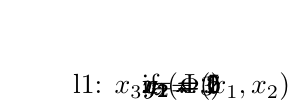
\begin{tikzpicture}
  \node (start) {};
  \node (a) {$x_1 = 5$};
  \node (b) {$x_2 = 6$};
  \node (c) {if ($\ldots$)};
  \node (d) {$y_1 = 1$};
  \node (e) {$y_2 = 2$};
  \node (f) {$z = 3$};
  \node (g) {l1: $x_3 = \Phi(x_1, x_2)$};
  \draw[->] (start) -- (a);
  \draw[->] (start) -- (b);
  \draw[->] (a) -- (g);
  \draw[->] (b) -- (c);
  \draw[->] (c) -- (d);
  \draw[->] (c) -- (e);
  \draw[->] (d) -- (f);
  \draw[->] (e) -- (f);
  \draw[->] (f) -- (g);
\end{tikzpicture}
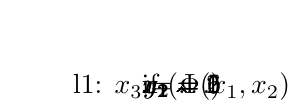
\begin{tikzpicture}
  \node (start) {};
  \node (a) {$x_1 = 5$};
  \node (b) {$x_2 = 6$};
  \node (c) {if ($\ldots$)};
  \node (d) {$y_1 = 1$};
  \node (e) {$y_2 = 2$};
  \node (g) {l1: $x_3 = \Phi(x_1, x_2)$};
  \draw[->] (start) -- (a);
  \draw[->] (start) -- (b);
  \draw[->] (a) -- (g);
  \draw[->] (b) -- (c);
  \draw[->] (c) -- (d);
  \draw[->] (c) -- (e);
  \draw[->] (d) -- (g);
  \draw[->] (e) -- (g);
\end{tikzpicture}
\caption{Optimising an SSA-form machine}
\label{fig:ssa_cfg1}
\end{figure}

\todo{Not actually sure how interesting this is, now that I've written it down.}

\subsection{Building write-side \StateMachines}

Once SLI has obtained the read-side \StateMachine, it can analyse it to determine which loads affect the ultimate prediction, and then compare this set to the dynamic model to determine which stores might potentially influence it.
The analysis must then consider all dynamic paths of $N^w$ instructions which contain at least one of those store operations.
As when building read-side \StateMachines, it would be possible to do this by enumerating all possible such paths and compiling each to an independent \StateMachine, but that would be extremely wasteful.
SLI uses a somewhat more intelligent approach.
The basic approach here is essentially the same as that used for read-side \StateMachines: convert the set of dynamic paths into a (hopefully much smaller) set of acyclic control-flow graphs and then compile those CFGs into \StateMachines.
The details of the algorithms used are, however, slightly different.

\subsubsection{Finding relevant stores}

The first phase of building the write-side \StateMachines is to determine which stores in the program might possibly be relevant.
These are the ones which might affect the result produced by the read-side \StateMachine.
Finding these is straightforward:

\begin{itemize}
\item
  Remove all of the optional annotations from the read-side \StateMachine.
  These are the side effects which provide additional information to the analysis but do not themselves affect the semantics of the \StateMachine, such as assert or stack-layout side effects.
\item
  Simplify the resulting machine down as far as possible.
  Removing annotations can sometimes enable further optimisations if, for instance, two path through the \StateMachine are identical except for inserting an additional intermediate function in the call stack and that intermediate function does not itself perform any relevant operations.
\item
  Find all of the memory load operations which remain the simplified machine.
\item
  Examine the model collected during the dynamic analysis phase to locate all of the stores which might access the same memory location as one of those loads.
  This effectively assumes both that the dynamic analysis phase has correctly captured the program's internal type system and that the program has a particular memory safety property.
  \todo{Say more.}
\end{itemize}

\subsubsection{Build write-side CFGs}
\todo{This has far more pages than it really deserves, although most
  of them are diagrams, so I guess it's not too bad.}

The input to this phase of the analysis is a set of potentially relevant static store instructions, and the analysis must build a collection of acyclic CFGs which cover all possible paths through the program which use at least one of those static instructions and which contain at most $N_w$ instructions.
\editorial{That's not quite the problem definition I used earlier, but it's a bit easier to describe.}

One important assumption here is that the set of potentially relevant store instructions is complete, in the sense that no instruction not in that set can influence the behaviour of the load machine (this follows from the assumption that the dynamic model is itself complete).
This implies that the only parts of the dynamic write path which are actually important are the potentially relevant store instructions; everything else simply acts to constrain the behaviour of those instructions.
That in turn means that it is safe to ignore any prefix or suffix of a dynamic path which does not involve any potentially-relevant store instructions, or, to put it another way, the store CFGs only need to represent dynamic paths which start and end with potentially-relevant instructions.
This is a useful simplification.

The algorithm begins by building a partial static CFG starting at each of the potentially-relevant store instructions and covering every instruction reachable within $N_w$ instructions of that point.
As with read-side CFGs, called functions are effectively inlined into each call site, and returns from the function containing the potentially-relevant store are handled by replacing the instruction with one with a synthesised call stack and restarting.
The CFGs generated by different starting instructions will often overlap; this is handled by sharing nodes between the relevant CFGs.
The resulting CFG is then trimmed to remove any instructions which cannot reach a potentially-relevant store within $N_w$ instructions.

At this point, the CFG represents a fragment of the program and contains every instruction which might be on one of the trimmed dynamic paths which need to be represented by the output CFG, and it only remains to remove any cycles from it.
As with read-side CFGs, this is accomplished by duplicating nodes so as to unroll loops until any path which uses the loop more than once must be longer than $N_w$ instructions and can hence be discarded.
There is, however, one important difference: in the read-side CFG, we are interested in any path which terminates at a specific point, whereas in the write-side CFG we need to preserve any path which starts and ends with any member of a set of interesting instructions.
This makes it more difficult to determine when a loop has been unrolled sufficiently, as it is no longer sufficient to just check the distance to a nominated target instruction.
SLI solves this problem by labelling each node in the graph with information about where it might occur in an interesting path.
This label consists of:

\begin{itemize}
\item
  For each possibly-relevant store, the minimum distance from that store to the labelled node.
\item
  For each possible-relevant store, the minimum distance from the labelled node to that store or any of its duplicates.
\end{itemize}

We only need to consider paths of length $N_w$ or less which start with one of the potentially-relevant stores and which end with a potentially-relevant store or one of its duplicates.
Therefore, if, for any node, the minimum of the first type of label plus the minimum of the second type of label exceeds $N_w$ the node can be safely discarded.
This allows us to break cycles once they have been unrolled far enough.

\begin{algorithmic}
  \STATE {Compute initial labelling of graph}
  \FORALL {$t$ in the set of potentially-relevant stores}
    \WHILE {graph rooted at $t$ is not cycle-free}
       \STATE $edge \gets findEdgeToBeBroken(t, \{\})$
       \STATE $newLabel \gets combineLabels(\text{current label of } edge.start, \text{current label of } edge.end)$
       \IF {$min(newLabel.minFrom) + min(newLabel.minTo) > N_w$}
           \STATE {remove $edge$}
       \ELSE
           \STATE $newNode <- \text{duplicate } edge.end$
           \FORALL {Edges $e$ leaving $edge.end$}
              \STATE {Create a new edge from $newNode$ to $e.end$}
           \ENDFOR
           \STATE {Set label of $newNode$ to $newLabel$}
           \STATE {Replace $edge$ with an edge from $edge.start$ to $newNode$}
       \ENDIF
    \ENDWHILE
  \ENDFOR
\end{algorithmic}

\begin{tikzpicture}
  \node (A) at (0,2) [TrueCfgInstr] {A};
  \node (B) [CfgInstr, below=of A] {B} edge [in=30,out=-30,loop] ();
  \node (C) [TrueCfgInstr, below=of B] {C};
  \draw[->] (A) -- (B);
  \draw[->] (B) -- (C);
  \draw[->] (C) to [bend left=90] (A) node (edge1) [right,midway] {~~~~~~~~};
  \begin{pgfonlayer}{bg}
    \node(box1) [fill=black!10,fit=(A) (B) (C) (edge1)] {};
  \end{pgfonlayer}
  \draw node [right=of box1] {
    \begin{tabular}{lcccc}
      labels & min to A & min from A & min to C & min from C\\
      A & 0 & 0 & 2 & 1\\
      B & 2 & 1 & 1 & 2\\
      C & 1 & 2 & 0 & 0\\
    \end{tabular}
  };
\end{tikzpicture}

\begin{tikzpicture}
  \node (A) at (0,2) [TrueCfgInstr] {A};
  \node (B) [CfgInstr, below=of A] {B};
  \node (B1) [NewCfgInstr, right=of B] {B1};
  \node (C) [TrueCfgInstr, below=of B] {C};
  \draw[->] (A) -- (B);
  \draw[->] (B) -- (C);
  \draw[->] (B) to [bend left=10] (B1);
  \draw[->,swungEdge] (B1) to [bend left=10] (B);
  \draw[->] (B1) -- (C);
  \draw[->] (C) to [bend left=90] (A) node (edge1) [right,midway] {~~~~~~~~};
  \begin{pgfonlayer}{bg}
    \node(box1) [fill=black!10,fit=(A) (B) (B1) (C) (edge1)] {};
  \end{pgfonlayer}
  \draw node [right=of box1] {
    \begin{tabular}{lcccc}
      labels & min to A & min from A & min to C & min from C\\
      A  & 0 & 0 & 2 & 1\\
      B  & 2 & 1 & 1 & 2\\
      C  & 1 & 2 & 0 & 0\\
      B1 & 2 & 2 & 1 & 3\\
    \end{tabular}
    (dupe B)
  };
\end{tikzpicture}

\begin{tikzpicture}
  \node (A) at (0,2) [TrueCfgInstr] {A};
  \node (B) [CfgInstr, below=of A] {B};
  \node (B1) [CfgInstr, right=of B] {B1};
  \node (C) [TrueCfgInstr, below=of B] {C};
  \node (A1) [NewCfgInstr,right=of C] {A1};
  \draw[->] (A) -- (B);
  \draw[->,swungEdge] (A1) -- (B);
  \draw[->] (B) -- (C);
  \draw[->] (B) to [bend left=10] (B1);
  \draw[->] (B1) -- (C);
  \draw[->] (B1) to [bend left=10] (B);
  \draw[->] (C) -- (A1);
  \begin{pgfonlayer}{bg}
    \node(box1) [fill=black!10,fit=(A) (B) (B1) (C) (edge1)] {};
  \end{pgfonlayer}
  \draw node [right=of box1] {
    \begin{tabular}{lcccc}
      labels & min to A & min from A & min to C & min from C\\
      A  & 0 & 0 & 2 & $\infty$\\
      A1 & 0 & 3 & 2 & 1\\
      B  & 2 & 1 & 1 & 2\\
      C  & 1 & 2 & 0 & 0\\
      B1 & 2 & 2 & 1 & 3\\
    \end{tabular}
    (dupe A)
  };
\end{tikzpicture}

\begin{tikzpicture}
  \node (A) at (0,2) [TrueCfgInstr] {A};
  \node (B) [CfgInstr, below=of A] {B};
  \node (B1) [CfgInstr, right=of B] {B1};
  \node (B2) [NewCfgInstr, right=of B1] {B2};
  \node (C) [TrueCfgInstr, below=of B] {C};
  \node (A1) [DupeCfgInstr,right=of C] {A1};
  \draw[->] (A) -- (B);
  \draw[->] (A1) -- (B);
  \draw[->] (B) -- (C);
  \draw[->] (B) -- (B1);
  \draw[->,swungEdge] (B1) to [bend left=10] (B2);
  \draw[->] (B1) -- (C);
  \draw[->] (B2) to [bend left=10] (B1);
  \draw[->] (B2) -- (C);
  \draw[->] (C) -- (A1);
  \begin{pgfonlayer}{bg}
    \node(box1) [fill=black!10,fit=(A) (A1) (B) (B1) (B2) (C) (edge1)] {};
  \end{pgfonlayer}
  \draw node [right=of box1] {
    \begin{tabular}{lcccc}
      labels & min to A & min from A & min to C & min from C\\
      A  & 0 & 0 & 2 & $\infty$\\
      A1 & 0 & 3 & 2 & 1\\
      B  & 2 & 1 & 1 & 2\\
      C  & 1 & 2 & 0 & 0\\
      B1 & 2 & 2 & 1 & 3\\
      B2 & 2 & 3 & 1 & 4\\
    \end{tabular}
  };
\end{tikzpicture}

\begin{tikzpicture}
  \node (A) at (0,2) [TrueCfgInstr] {A};
  \node (B) [CfgInstr, below=of A] {B};
  \node (B1) [CfgInstr, right=of B] {B1};
  \node (B2) [CfgInstr, right=of B1] {B2};
  \node (A1) [DupeCfgInstr,right=of C] {A1};
  \node (C) [TrueCfgInstr, below=of B] {C};
  \node (B3) [NewCfgInstr, below=of A1] {B3};
  \draw[->] (A) -- (B);
  \draw[->,swungEdge] (A1) -- (B3);
  \draw[->] (B) -- (C);
  \draw[->] (B) -- (B1);
  \draw[->] (B1) to [bend left=10] (B2);
  \draw[->] (B1) -- (C);
  \draw[->] (B2) to [bend left=10] (B1);
  \draw[->] (B2) -- (C);
  \draw[->] (B3) -- (C);
  \draw[->] (B3) to [bend right=45] (B1);
  \draw[->] (C) -- (A1);
  \begin{pgfonlayer}{bg}
    \node(box1) [fill=black!10,fit=(A) (A1) (B) (B1) (B2) (B3) (C) (edge1)] {};
  \end{pgfonlayer}
  \draw node [right=of box1] {
    \begin{tabular}{lcccc}
      labels & min to A & min from A & min to C & min from C\\
      A  & 0 & 0 & 2 & $\infty$\\
      A1 & 0 & 3 & 2 & 1\\
      B  & 2 & 1 & 1 & $\infty$\\
      C  & 1 & 2 & 0 & 0\\
      B1 & 2 & 2 & 1 & 3\\
      B2 & 2 & 3 & 1 & 4\\
      B3 & 2 & 4 & 1 & 2\\
    \end{tabular}
  };
\end{tikzpicture}

\begin{tikzpicture}
  \node (A) at (0,2) [TrueCfgInstr] {A};
  \node (B) [CfgInstr, below=of A] {B};
  \node (B1) [CfgInstr, right=of B] {B1};
  \node (B2) [CfgInstr, right=of B1] {B2};
  \node (A1) [DupeCfgInstr,right=of C] {A1};
  \node (C) [TrueCfgInstr, below=of B] {C};
  \node (B3) [CfgInstr, below=of A1] {B3};
  \draw[->] (A) -- (B);
  \draw[->] (A1) -- (B3);
  \draw[->] (B) -- (C);
  \draw[->] (B) -- (B1);
  \draw[->] (B1) to [bend left=10] (B2);
  \draw[->] (B1) -- (C);
  \draw[->] (B2) to [bend left=10] (B1);
  \draw[->,killEdge] (B2) to [bend left=10] (B1);
  \draw[->] (B2) -- (C);
  \draw[->] (B3) -- (C);
  \draw[->] (B3) to [bend right=45] (B1);
  \draw[->] (C) -- (A1);
  \begin{pgfonlayer}{bg}
    \node(box1) [fill=black!10,fit=(A) (A1) (B) (B1) (B2) (B3) (C) (edge1)] {};
  \end{pgfonlayer}
  \draw node [right=of box1] {
    \begin{tabular}{lcccc}
      labels & min to A & min from A & min to C & min from C\\
      A  & 0 & 0 & 2 & $\infty$\\
      A1 & 0 & 3 & 2 & 1\\
      B  & 2 & 1 & 1 & $\infty$\\
      C  & 1 & 2 & 0 & 0\\
      B1 & 2 & 2 & 1 & 3\\
      B2 & 2 & 3 & 1 & 4\\
      New label & 2 & 4 & 1 & 5\\
    \end{tabular}
  };
\end{tikzpicture}

\begin{tikzpicture}
  \node (A) at (0,2) [TrueCfgInstr] {A};
  \node (B) [CfgInstr, below=of A] {B};
  \node (B1) [CfgInstr, right=of B] {B1};
  \node (B2) [CfgInstr, right=of B1] {B2};
  \node (A1) [DupeCfgInstr,right=of C] {A1};
  \node (C) [TrueCfgInstr, below=of B] {C};
  \node (B3) [CfgInstr, below=of A1] {B3};
  \node (C1) [NewCfgInstr, below=of B3] {C1};
  \draw[->] (A) -- (B);
  \draw[->] (A1) -- (B3);
  \draw[->] (B) -- (C);
  \draw[->] (B) -- (B1);
  \draw[->] (B1) -- (B2);
  \draw[->] (B1) -- (C);
  \draw[->] (B2) -- (C);
  \draw[->] (B3) to [bend left=45] (B1);
  \draw[->] (C) -- (A1);
  \draw[->] (C1) to [bend right=90] (A1);
  \draw[->,swungEdge] (B3) -- (C1);
  \begin{pgfonlayer}{bg}
    \node(box1) [fill=black!10,fit=(A) (A1) (B) (B1) (B2) (B3) (C) (C1) (edge1)] {};
  \end{pgfonlayer}
  \draw node [right=of box1] {
    \begin{tabular}{lcccc}
      labels & min to A & min from A & min to C & min from C\\
      A  & 0 & 0 & 2 & $\infty$\\
      A1 & 0 & 3 & 2 & 1\\
      B  & 2 & 1 & 1 & $\infty$\\
      C  & 1 & 2 & 0 & 0\\
      B1 & 2 & 2 & 1 & 3\\
      B2 & 2 & 3 & 1 & 4\\
      C3 & 1 & 4 & 0 & 3\\
    \end{tabular}
  };
\end{tikzpicture}

\begin{tikzpicture}
  \node (A) at (0,2) [TrueCfgInstr] {A};
  \node (B) [CfgInstr, below=of A] {B};
  \node (B1) [CfgInstr, right=of B] {B1};
  \node (B2) [CfgInstr, right=of B1] {B2};
  \node (A1) [DupeCfgInstr,right=of C] {A1};
  \node (C) [TrueCfgInstr, below=of B] {C};
  \node (B3) [CfgInstr, below=of A1] {B3};
  \node (C1) [DupeCfgInstr, below=of B3] {C1};
  \node (B4) [NewCfgInstr, right=of B3] {B4};
  \draw[->] (A) -- (B);
  \draw[->] (A1) -- (B3);
  \draw[->] (B) -- (C);
  \draw[->] (B) -- (B1);
  \draw[->] (B1) -- (B2);
  \draw[->] (B1) -- (C);
  \draw[->] (B2) -- (C);
  \draw[->,swungEdge] (B3) -- (B4);
  \draw[->] (C) -- (A1);
  \draw[->] (C1) to [bend right=45] (A1);
  \draw[->] (B3) -- (C1);
  \draw[->] (B4) -- (C);
  \draw[->] (B4) -- (B2);
  \begin{pgfonlayer}{bg}
    \node(box1) [fill=black!10,fit=(A) (A1) (B) (B1) (B2) (B3) (C) (C1) (edge1)] {};
  \end{pgfonlayer}
  \draw node [right=of box1] {
    \begin{tabular}{lcccc}
      labels & min to A & min from A & min to C & min from C\\
      A  & 0 & 0 & 2 & $\infty$\\
      A1 & 0 & 3 & 2 & 1\\
      B  & 2 & 1 & 1 & $\infty$\\
      C  & 1 & 2 & 0 & 0\\
      B1 & 2 & 2 & 1 & $\infty$\\
      B2 & 2 & 3 & 1 & 4\\
      C3 & 1 & 4 & 0 & 3\\
      B4 & 2 & 5 & 1 & 3\\
    \end{tabular}
  };
\end{tikzpicture}

\begin{tikzpicture}
  \node (A) at (0,2) [TrueCfgInstr] {A};
  \node (B) [CfgInstr, below=of A] {B};
  \node (B1) [CfgInstr, right=of B] {B1};
  \node (B2) [CfgInstr, right=of B1] {B2};
  \node (A1) [DupeCfgInstr,right=of C] {A1};
  \node (C) [TrueCfgInstr, below=of B] {C};
  \node (B3) [CfgInstr, below=of A1] {B3};
  \node (C1) [DupeCfgInstr, below=of B3] {C1};
  \node (B4) [CfgInstr, right=of B3] {B4};
  \node (A2) [NewCfgInstr, left=of C1] {A2};
  \draw[->] (A) -- (B);
  \draw[->] (A1) -- (B3);
  \draw[->] (B) -- (C);
  \draw[->] (B) -- (B1);
  \draw[->] (B1) -- (B2);
  \draw[->] (B1) -- (C);
  \draw[->] (B2) -- (C);
  \draw[->] (B3) -- (B4);
  \draw[->] (C) -- (A1);
  \draw[->,swungEdge] (C1) -- (A2);
  \draw[->] (B3) -- (C1);
  \draw[->] (B4) -- (C);
  \draw[->] (B4) -- (B2);
  \draw[->] (A2) -- (B3);
  \begin{pgfonlayer}{bg}
    \node(box1) [fill=black!10,fit=(A) (A1) (A2) (B) (B1) (B2) (B3) (C) (C1) (edge1)] {};
  \end{pgfonlayer}
  \draw node [right=of box1] {
    \begin{tabular}{lcccc}
      labels & min to A & min from A & min to C & min from C\\
      A  & 0 & 0 & 2 & $\infty$\\
      A1 & 0 & 3 & 2 & 1\\
      B  & 2 & 1 & 1 & $\infty$\\
      C  & 1 & 2 & 0 & 0\\
      B1 & 2 & 2 & 1 & $\infty$\\
      B2 & 2 & 3 & 1 & 4\\
      C3 & 1 & 4 & 0 & 3\\
      B4 & 2 & 5 & 1 & 3\\
      A2 & 0 & 6 & 2 & 4\\
    \end{tabular}
  };
\end{tikzpicture}

\begin{tikzpicture}
  \node (A) at (0,2) [TrueCfgInstr] {A};
  \node (B) [CfgInstr, below=of A] {B};
  \node (B1) [CfgInstr, right=of B] {B1};
  \node (B2) [CfgInstr, right=of B1] {B2};
  \node (A1) [DupeCfgInstr,right=of C] {A1};
  \node (C) [TrueCfgInstr, below=of B] {C};
  \node (B3) [CfgInstr, below=of A1] {B3};
  \node (C1) [DupeCfgInstr, below=of B3] {C1};
  \node (B4) [CfgInstr, right=of B3] {B4};
  \node (A2) [DupeCfgInstr, left=of C1] {A2};
  \node (C2) [NewCfgInstr, below=of B4] {C2};
  \draw[->] (A) -- (B);
  \draw[->] (A1) -- (B3);
  \draw[->] (B) -- (C);
  \draw[->] (B) -- (B1);
  \draw[->] (B1) -- (B2);
  \draw[->] (B1) -- (C);
  \draw[->] (B2) -- (C);
  \draw[->] (B3) -- (B4);
  \draw[->] (C) -- (A1);
  \draw[->] (C1) -- (A2);
  \draw[->] (B3) -- (C1);
  \draw[->,swungEdge] (B4) -- (C2);
  \draw[->] (B4) -- (B2);
  \draw[->] (A2) -- (B3);
  \draw[->] (C2) -- (A1);
  \begin{pgfonlayer}{bg}
    \node(box1) [fill=black!10,fit=(A) (A1) (A2) (B) (B1) (B2) (B3) (C) (C1) (C2) (edge1)] {};
  \end{pgfonlayer}
  \draw node [right=of box1] {
    \begin{tabular}{lcccc}
      labels & min to A & min from A & min to C & min from C\\
      A  & 0 & 0 & 2 & $\infty$\\
      A1 & 0 & 3 & 2 & 1\\
      B  & 2 & 1 & 1 & $\infty$\\
      C  & 1 & 2 & 0 & 0\\
      B1 & 2 & 2 & 1 & $\infty$\\
      B2 & 2 & 3 & 1 & 4\\
      C3 & 1 & 4 & 0 & 3\\
      B4 & 2 & 5 & 1 & 3\\
      A2 & 0 & 6 & 2 & 4\\
      C2 & 1 & 6 & 0 & 4\\
    \end{tabular}
  };
\end{tikzpicture}

\begin{tikzpicture}
  \node (A) at (0,2) [TrueCfgInstr] {A};
  \node (B) [CfgInstr, below=of A] {B};
  \node (B1) [CfgInstr, right=of B] {B1};
  \node (B2) [CfgInstr, right=of B1] {B2};
  \node (A1) [DupeCfgInstr,right=of C] {A1};
  \node (C) [TrueCfgInstr, below=of B] {C};
  \node (B3) [CfgInstr, below=of A1] {B3};
  \node (C1) [DupeCfgInstr, below=of B3] {C1};
  \node (B4) [CfgInstr, right=of B3] {B4};
  \node (A2) [DupeCfgInstr, left=of C1] {A2};
  \node (C2) [DupeCfgInstr, below=of B4] {C2};
  \draw[->] (A) -- (B);
  \draw[->] (A1) -- (B3);
  \draw[->] (B) -- (C);
  \draw[->] (B) -- (B1);
  \draw[->] (B1) -- (B2);
  \draw[->] (B1) -- (C);
  \draw[->] (B2) -- (C);
  \draw[->] (B3) -- (B4);
  \draw[->] (C) -- (A1);
  \draw[->] (C1) -- (A2);
  \draw[->] (B3) -- (C1);
  \draw[->] (B4) -- (C2);
  \draw[->] (B4) -- (B2);
  \draw[->] (A2) -- (B3);
  \draw[->,killEdge] (A2) -- (B3);
  \draw[->] (C2) -- (A1);
  \begin{pgfonlayer}{bg}
    \node(box1) [fill=black!10,fit=(A) (A1) (A2) (B) (B1) (B2) (B3) (C) (C1) (C2) (edge1)] {};
  \end{pgfonlayer}
  \draw node [right=of box1] {
    \begin{tabular}{lcccc}
      labels & min to A & min from A & min to C & min from C\\
      A  & 0 & 0 & 2 & $\infty$\\
      A1 & 0 & 3 & 2 & 1\\
      B  & 2 & 1 & 1 & $\infty$\\
      C  & 1 & 2 & 0 & 0\\
      B1 & 2 & 2 & 1 & $\infty$\\
      B2 & 2 & 3 & 1 & 4\\
      C3 & 1 & 4 & 0 & 3\\
      B4 & 2 & 5 & 1 & 3\\
      A2 & 0 & 6 & 2 & 4\\
      C2 & 1 & 6 & 0 & 4\\
      New label & 2 & 7 & 1 & 5\\
    \end{tabular}\\
    (Dupe B5)
  };
\end{tikzpicture}

\begin{tikzpicture}
  \node (A) at (0,2) [TrueCfgInstr] {A};
  \node (B) [CfgInstr, below=of A] {B};
  \node (B1) [CfgInstr, right=of B] {B1};
  \node (B2) [CfgInstr, right=of B1] {B2};
  \node (A1) [DupeCfgInstr,right=of C] {A1};
  \node (C) [TrueCfgInstr, below=of B] {C};
  \node (B3) [CfgInstr, below=of A1] {B3};
  \node (C1) [DupeCfgInstr, below=of B3] {C1};
  \node (B4) [CfgInstr, right=of B3] {B4};
  \node (A2) [DupeCfgInstr, left=of C1] {A2};
  \node (C2) [DupeCfgInstr, below=of B4] {C2};
  \draw[->] (A) -- (B);
  \draw[->] (A1) -- (B3);
  \draw[->] (B) -- (C);
  \draw[->] (B) -- (B1);
  \draw[->] (B1) -- (B2);
  \draw[->] (B1) -- (C);
  \draw[->] (B2) -- (C);
  \draw[->] (B3) -- (B4);
  \draw[->] (C) -- (A1);
  \draw[->] (C1) -- (A2);
  \draw[->] (B3) -- (C1);
  \draw[->] (B4) -- (C2);
  \draw[->] (B4) -- (B2);
  \draw[->] (C2) -- (A1);
  \draw[->,killEdge] (C2) -- (A1);
  \begin{pgfonlayer}{bg}
    \node(box1) [fill=black!10,fit=(A) (A1) (A2) (B) (B1) (B2) (B3) (C) (C1) (C2) (edge1)] {};
  \end{pgfonlayer}
  \draw node [right=of box1] {
    \begin{tabular}{lcccc}
      labels & min to A & min from A & min to C & min from C\\
      A  & 0 & 0 & 2 & $\infty$\\
      A1 & 0 & 3 & 2 & 1\\
      B  & 2 & 1 & 1 & $\infty$\\
      C  & 1 & 2 & 0 & 0\\
      B1 & 2 & 2 & 1 & $\infty$\\
      B2 & 2 & 3 & 1 & 4\\
      C3 & 1 & 4 & 0 & 3\\
      B4 & 2 & 5 & 1 & 3\\
      A2 & 0 & 6 & 2 & 4\\
      C2 & 1 & 6 & 0 & 4\\
      New label & 0 & 7 & 2 & 5\\
    \end{tabular}\\
    (Dupe A1)
  };
\end{tikzpicture}

\begin{tikzpicture}
  \node (A) at (0,2) [TrueCfgInstr] {A};
  \node (B) [CfgInstr, below=of A] {B};
  \node (B1) [CfgInstr, right=of B] {B1};
  \node (B2) [CfgInstr, right=of B1] {B2};
  \node (A1) [DupeCfgInstr,right=of C] {A1};
  \node (C) [TrueCfgInstr, below=of B] {C};
  \node (B3) [CfgInstr, below=of A1] {B3};
  \node (C1) [DupeCfgInstr, below=of B3] {C1};
  \node (B4) [CfgInstr, right=of B3] {B4};
  \node (A2) [DupeCfgInstr, left=of C1] {A2};
  \node (C2) [DupeCfgInstr, below=of B4] {C2};
  \node (C3) [NewCfgInstr, right=of A1] {C3};
  \draw[->] (A) -- (B);
  \draw[->] (A1) -- (B3);
  \draw[->] (B) -- (C);
  \draw[->] (B) -- (B1);
  \draw[->] (B1) -- (B2);
  \draw[->] (B1) -- (C);
  \draw[->,swungEdge] (B2) -- (C3);
  \draw[->] (B3) -- (B4);
  \draw[->] (C) -- (A1);
  \draw[->] (C1) -- (A2);
  \draw[->] (B3) -- (C1);
  \draw[->] (B4) -- (C2);
  \draw[->] (B4) to [bend left=45] (B2);
  \draw[->] (C3) -- (A1);
  \begin{pgfonlayer}{bg}
    \node(box1) [fill=black!10,fit=(A) (A1) (A2) (B) (B1) (B2) (B3) (C) (C1) (C2) (C3) (edge1)] {};
  \end{pgfonlayer}
  \draw node [right=of box1] {
    \begin{tabular}{lcccc}
      labels & min to A & min from A & min to C & min from C\\
      A  & 0 & 0 & 2 & $\infty$\\
      A1 & 0 & 3 & 2 & 1\\
      B  & 2 & 1 & 1 & $\infty$\\
      C  & 1 & 2 & 0 & 0\\
      B1 & 2 & 2 & 1 & $\infty$\\
      B2 & 2 & 3 & 1 & 4\\
      C3 & 1 & 4 & 0 & 3\\
      B4 & 2 & 5 & 1 & 3\\
      A2 & 0 & 6 & 2 & 4\\
      C2 & 1 & 6 & 0 & 4\\
      C3 & 1 & 4 & 0 & 5\\
    \end{tabular}
  };
\end{tikzpicture}

\begin{tikzpicture}
  \node (A) at (0,2) [TrueCfgInstr] {A};
  \node (B) [CfgInstr, below=of A] {B};
  \node (B1) [CfgInstr, right=of B] {B1};
  \node (B2) [CfgInstr, right=of B1] {B2};
  \node (A1) [DupeCfgInstr,right=of C] {A1};
  \node (C) [TrueCfgInstr, below=of B] {C};
  \node (B3) [CfgInstr, below=of A1] {B3};
  \node (C1) [DupeCfgInstr, below=of B3] {C1};
  \node (B4) [CfgInstr, right=of B3] {B4};
  \node (A2) [DupeCfgInstr, left=of C1] {A2};
  \node (C2) [DupeCfgInstr, below=of B4] {C2};
  \node (C3) [DupeCfgInstr, right=of A1] {C3};
  \draw[->] (A) -- (B);
  \draw[->] (A1) -- (B3);
  \draw[->] (B) -- (C);
  \draw[->] (B) -- (B1);
  \draw[->] (B1) -- (B2);
  \draw[->] (B1) -- (C);
  \draw[->] (B2) -- (C3);
  \draw[->] (B3) -- (B4);
  \draw[->] (C) -- (A1);
  \draw[->] (C1) -- (A2);
  \draw[->] (B3) -- (C1);
  \draw[->] (B4) -- (C2);
  \draw[->] (B4) to [bend left=45] (B2);
  \draw[->,killEdge] (B4) to [bend left=45] (B2);
  \draw[->] (C3) -- (A1);
  \begin{pgfonlayer}{bg}
    \node(box1) [fill=black!10,fit=(A) (A1) (A2) (B) (B1) (B2) (B3) (C) (C1) (C2) (C3) (edge1)] {};
  \end{pgfonlayer}
  \draw node [right=of box1] {
    \begin{tabular}{lcccc}
      labels & min to A & min from A & min to C & min from C\\
      A  & 0 & 0 & 2 & $\infty$\\
      A1 & 0 & 3 & 2 & 1\\
      B  & 2 & 1 & 1 & $\infty$\\
      C  & 1 & 2 & 0 & 0\\
      B1 & 2 & 2 & 1 & $\infty$\\
      B2 & 2 & 3 & 1 & $\infty$\\
      C3 & 1 & 4 & 0 & $\infty$\\
      B4 & 2 & 5 & 1 & 3\\
      A2 & 0 & 6 & 2 & 4\\
      C2 & 1 & 6 & 0 & 4\\
      C3 & 1 & 4 & 0 & 5\\
      New label & 2 & 6 & 1 & 4\\
    \end{tabular}
  };
\end{tikzpicture}

\begin{tikzpicture}
  \node (A) at (0,2) [TrueCfgInstr] {A};
  \node (B) [CfgInstr, below=of A] {B};
  \node (B1) [CfgInstr, right=of B] {B1};
  \node (B2) [CfgInstr, right=of B1] {B2};
  \node (A1) [DupeCfgInstr,right=of C] {A1};
  \node (C) [TrueCfgInstr, below=of B] {C};
  \node (B3) [CfgInstr, below=of A1] {B3};
  \node (C1) [DupeCfgInstr, below=of B3] {C1};
  \node (B4) [CfgInstr, right=of B3] {B4};
  \node (A2) [DupeCfgInstr, left=of C1] {A2};
  \node (C2) [DupeCfgInstr, below=of B4] {C2};
  \node (C3) [DupeCfgInstr, right=of A1] {C3};
  \draw[->] (A) -- (B);
  \draw[->] (A1) -- (B3);
  \draw[->] (B) -- (C);
  \draw[->] (B) -- (B1);
  \draw[->] (B1) -- (B2);
  \draw[->] (B1) -- (C);
  \draw[->] (B2) -- (C3);
  \draw[->] (B3) -- (B4);
  \draw[->] (C) -- (A1);
  \draw[->] (C1) -- (A2);
  \draw[->] (B3) -- (C1);
  \draw[->] (B4) -- (C2);
  \draw[->] (C3) -- (A1);
  \draw[->,killEdge] (C3) -- (A1);
  \begin{pgfonlayer}{bg}
    \node(box1) [fill=black!10,fit=(A) (A1) (A2) (B) (B1) (B2) (B3) (C) (C1) (C2) (C3) (edge1)] {};
  \end{pgfonlayer}
  \draw node [right=of box1] {
    \begin{tabular}{lcccc}
      labels & min to A & min from A & min to C & min from C\\
      A  & 0 & 0 & 2 & $\infty$\\
      A1 & 0 & 3 & 2 & 1\\
      B  & 2 & 1 & 1 & $\infty$\\
      C  & 1 & 2 & 0 & 0\\
      B1 & 2 & 2 & 1 & $\infty$\\
      B2 & 2 & 3 & 1 & $\infty$\\
      C3 & 1 & 4 & 0 & $\infty$\\
      B4 & 2 & 5 & 1 & 3\\
      A2 & 0 & 6 & 2 & 4\\
      C2 & 1 & 6 & 0 & 4\\
      C3 & 1 & 4 & 0 & 5\\
      New label & 0 & 5 & 2 & 6\\
    \end{tabular}
  };
\end{tikzpicture}

\begin{tikzpicture}
  \node (A) at (0,2) [TrueCfgInstr] {A};
  \node (B) [CfgInstr, below=of A] {B};
  \node (B1) [CfgInstr, right=of B] {B1};
  \node (B2) [CfgInstr, right=of B1] {B2};
  \node (A1) [DupeCfgInstr,right=of C] {A1};
  \node (C) [TrueCfgInstr, below=of B] {C};
  \node (B3) [CfgInstr, below=of A1] {B3};
  \node (C1) [DupeCfgInstr, below=of B3] {C1};
  \node (B4) [CfgInstr, right=of B3] {B4};
  \node (A2) [DupeCfgInstr, left=of C1] {A2};
  \node (C2) [DupeCfgInstr, below=of B4] {C2};
  \node (C3) [DupeCfgInstr, right=of A1] {C3};
  \draw[->] (A) -- (B);
  \draw[->] (A1) -- (B3);
  \draw[->] (B) -- (C);
  \draw[->] (B) -- (B1);
  \draw[->] (B1) -- (B2);
  \draw[->] (B1) -- (C);
  \draw[->] (B2) -- (C3);
  \draw[->] (B3) -- (B4);
  \draw[->] (C) -- (A1);
  \draw[->] (C1) -- (A2);
  \draw[->] (B3) -- (C1);
  \draw[->] (B4) -- (C2);
  \begin{pgfonlayer}{bg}
    \node(box1) [fill=black!10,fit=(A) (A1) (A2) (B) (B1) (B2) (B3) (C) (C1) (C2) (C3) (edge1)] {};
  \end{pgfonlayer}
  \draw node [right=of box1] {
    \begin{tabular}{lcccc}
      labels & min to A & min from A & min to C & min from C\\
      A  & 0 & 0 & 2 & $\infty$\\
      A1 & 0 & 3 & 2 & 1\\
      B  & 2 & 1 & 1 & $\infty$\\
      C  & 1 & 2 & 0 & 0\\
      B1 & 2 & 2 & 1 & $\infty$\\
      B2 & 2 & 3 & 1 & $\infty$\\
      C3 & 1 & 4 & 0 & $\infty$\\
      B4 & 2 & 5 & 1 & 3\\
      A2 & 0 & 6 & 2 & 4\\
      C2 & 1 & 6 & 0 & 4\\
      C3 & 1 & 4 & 0 & 5\\
    \end{tabular}
  };
\end{tikzpicture}


\subsection{Converting pairs of \StateMachines into verification conditions}

We now convert the pair of \StateMachines into a form of verification condition; that is, a predicate on the program's state which is satisfiable when the program contains a bug of the type being investigated\editorial{That isn't quite the usual definition of a verification condition.}.
SLI's completeness property is that if every possible \StateMachine pair which could be generated by the above algorithm is generated and each one is successfully converted to a verification condition (i.e. no part of the analysis times out), and none of the verification conditions are satisfiable, and the dynamic analysis is complete, the program will not contain any bugs of the class being investigated.

At a high level, the verification conditions are produced by considering each of the clauses of the bug definition in section~\todo{...} in turn, converting each into a \StateMachine, and then using symbolic execution to build a predicate saying when that clause might be satisfied.
These clause-conditions are then combined to produce the final verification condition for the original \StateMachine pair.

The rules for building each clause-condition are as follows:

\begin{itemize}
\item P valid -- \editorial{not sure what I'm going to say here -- P doesn't really exist at this stage, so this clause doesn't really make sense here.}
\item R valid -- true by construction of read machine, so the clause condition is just $1$.
\item W valid -- true by construction of write machine, so the clause condition is just $1$.
\item
  R atomic -- this rule states that the read \StateMachine must predict survival when run atomically.
  The \StateMachine to symbolically execute is then just the read-side \StateMachine, and the clause constraint is the rule which the symbolic executor derives for when the \StateMachine will survive.
\item
  W atomic -- this rule states that running the read \StateMachine after the write one must also predict survival.
  For this clause, we symbolically execute the concatenation of the two \StateMachines, and again the clause constraint is the rule when the \StateMachine will survive.
\item
  Crash possible -- this rule states that running the read and write \StateMachines in parallel must sometimes predict a crash.
  For this clause, we symbolically execute the cross-product parallel composition of the two \StateMachines.
  This time, the clause constraint is the rule for when the \StateMachine will crash.
\item
  W isolation -- used extensively when deriving write machine, to the extent that there's rarely any additional useful information to extract by this stage in the pipeline.
\item
  Concurrent -- model of program isn't strong enough to say anything useful about it.
\end{itemize}

We therefore produce three clause constraints for each \StateMachine pair, and must report a bug if they are simultaneously satisfiable.
As a minor optimisation, SLI assumes the R atomic clause is true when deriving the W atomic and crash clauses, and assumes that the W atomic clause is true when deriving the crash possible clause.

\subsubsection{Symbolically executing machines}

SLI uses a simple symbolic execution engine to evaluate machines and
determine when \StateMachines will crash.  The details of this are
fairly standard, and I only give a brief overview
here\editorial{\emph{Should} only give a brief overview; this ended up
  much more detailed than I'd expected.}.  The core data structure
used by the execution engine is a queue of (mostly) symbolic
configurations which the \StateMachine might occupy, and the main
operation is to take a state out of this queue, determine what the
\StateMachine might do next, and possibly add some additional
configurations to the queue to explore further.  Each configuration
contains:

\begin{itemize}
\item
  A mapping from temporary variable identifiers to the (symbolic) values of those variables.
\item
  A reference to the {\StateMachine}'s current (non-symbolic) state.
\item
  The order in which those temporaries were assigned to.
  As discussed in \S~\ref{sect:ssa}, SLI uses a slightly unusual form of single static assignment in which $\Phi$ nodes select their input variable based on which was assigned to most recently, rather than based on the preceding control flow, and this keeping track of that ordering allows that semantics to be implemented simply.
\item
  A log of all of the memory stores issued by the \StateMachine so far.
\item
  The current assumption.
  This is simply the conjunction of all of the conditions which are known to be true at this point in the execution.
\item
  The current ``path'' assumption.
  This is the subset of the current assumption which was introduced during the machine's execution.
  In other words, it is all of the things which are known to be true at this point in the execution but which were not known to be true at the start of the execution.
  This is often useful when building verification conditions, as discussed below.

  An alternative design would instead keep the path assumption and the initial assumption completely separate, and get rid of the current assumption, but this is slightly more convenient\editorial{think harder.}.
\end{itemize}\editorial{Plus some debug crap, but we don't care about that here.}

There are three possible outcomes from an execution: crash, survive, or escape.
The first two are obvious.
An escaping result indicates that the \StateMachine behaved in a way which indicates that this execution is not one of the ones which are of interest to the current bug.
This might, for instance, be because an assertion fails, or because a memory access (other than the one being investigated) dereferenced bad memory.
The exact treatment of escaping executions depends on how the results of the symbolic execution are to be used.

Implementing the various types of \StateMachine operation is straightforward:

\begin{itemize}
\item[cond]
  Check whether the assumption allows the condition to be simplified to a constant.
  If it does, simplify advance to the appropriate successor state.
  Otherwise, create two new successor configurations, moving one to the state's condition-true successor state and the other to the condition-false one and adding either the constraint (for the condition-true successor) or its inverse (for the condition-false one) to the current assumption and the path assumption.
\item[assert]
  Check whether the assumption allows the asserted value to be reduced to a constant.
  If it can, and that constant is one, simply move to the assertion's successor state.
  If the constant is zero, the execution escapes.
  Otherwise, if the asserted expression cannot be reduced to a constant, it is added to the current assumption and path assumption and the execution moves to the successor state.
\item[copy]
  Simplify the right-hand side of the copy as far as possible using the current assumption and then copy it to the appropriate place in the temporary variable table.
  The current assumption is then rewritten to replace any instances of the left-hand side of the copy with the simplified version of the right-hand side.
  The path assumption is not rewritten, and neither are the values of any of the other temporary values.
  \todo{I'm at least half convinced that this doesn't actually matter any more, due to changes elsewhere in the analysis pipeline.  Need to check that.}
\item[store]
  Assert that the pointer stored to is itself valid and then add the store to the log of issued stores.
\item[load]
  Assert that the pointer to be loaded is itself valid.
  Look through the log of issued stores, checking each one to see whether it might be storing to the location loaded by the load.
  If the load is unambiguously satisfied by a single store then create a single successor configuration then copy the value stored into the temporary variable targeted by the load using the same mechanism as used for copy side-effects.
  Otherwise, create one for each possible store, and potentially also one in which the load returns the initial value of memory.
\item[phi]
  Essentially as far copy operations.
\item
  Every operation is a no-op in the interpreter and simply moves to the next state.
  In particular, the execution engine ignores operations such as ``StartLayout'' and ``PointerAliasing'' which simply provide additional hints to the various \StateMachine simplification phases.
\end{itemize}

\todo{Possibly important that this uses the simplifier rather than the sat checker to see whether things reduce to a constant.}

Asserting that pointers are valid before performing memory operations is perhaps slightly surprising, as it means that the execution engine will never consider paths which crash due to dereferencing bad pointers.
This may appear odd in a system designed to investigate crashes due to dereferencing bad pointers.
However, it simply reflects the fact that, at this stage, SLI is only interested in a single possibly-crashing instruction, and so crashes at memory accesses prior to that one need to be ignored; asserting that dereferenced pointers are valid achieves that.
The interesting instruction itself is encoded without an explicit memory-accessing state (see \S~\todo{...}), so crashes there will not be affected by these assertions.

\todo{At one point, the execution engine was the reason we needed dynamic single assignment form.  I can't really see why it depends on it now, though, so that might be worth looking at more.}

\subsubsection{R atomic}

This rule states that the read machine must run to completion without crashing if run in isolation.
Once the read machine has been completely determined, this is in effect a condition on the states of the program which have to be considered: if the read machine would crash when run atomically in state S, any concurrency-related bugs detected starting from state S are highly unlikely to be interesting.
The first phase of building the verification condition is to build the condition.
To do so, the analysis first simplifies the probe machine on the assumption that it is running atomically and then symbolically executes it.
The constraint is then the conjunction of the inverses of the path conditions to reach crashing states.
Escaping executions are treated as crashing ones at this stage, so that they will not be considered by later stages of the analysis.

Path explosion: once you're assuming that the machine is completely atomic the state machine simplifier turns most machines into a simple predicate on the initial state and so the symbolic execution is pretty much trivial and there aren't really any paths to explode.
The main exception is where Phi nodes prevent us from simplifying control flow as far as we'd like.
Aliasing can also be an issue, but much less often than you'd expect.

\subsection{W atomic}

This rule requires that the read machine does not crash if run after the write machine has completed.
This, again, is about restricting the analysis to only consider bugs which are due to concurrency, and not any crashes which might be caused by other bugs.
For this rule, the analysis first concatenates the two machines by replacing the terminal states of the write machine with the first state in the read machine.
The resulting machine is then simplified and interpreted.
In this case, the symbolic execution engine is allowed to assume that the R atomic condition holds while performing this interpretation
The resulting path conditions are converted into a validity predicate in essentially the same way as they are for the R atomic rule.

Path explosion: again modest at this stage.
Most store machines just consist of a small number of store instructions (usually one, almost never more than three) and no control flow, and so we're effectively repeating the R atomic calculations in a slightly different initial state.
The aliasing problems are more complicated here but generally still not intractable.

\subsection{Crash possible}

This rule requires that the read machine must sometimes crash if run in parallel with the store machine.
To build this predicate, the analysis builds a new \StateMachine which is the cross product of the input read and write machines and then interprets that.
For this interpretation, escaping states, where assertions fail, are assumed to survive.
The final result is the disjunction of all of the path conditions which reach crashing states; combined with the validity condition, this describes all of the states which might exhibit a bug of the target class.

Complication: we arrange to build the machines in a way which avoids running either machine to completion in isolation.

I'm going to have to describe the algorithm here, because it's a little bit subtle.

Interesting properties of the algorithm:

\begin{itemize}
\item
  Needs to maintain atomic blocks.
\item
  Need to avoid considering the cases where either machine runs to completion before the other one starts.
\item
  Avoid considering both orderings of a load-store pair if they can't ever possibly access the same memory location.
  Slight complication: need to look past the current memory access to see if there's anything after it which might possibly race in an interesting way.
\item
  When you do need to consider both orderings, one of the orderings asserts that the two accesses access the same location and the other one doesn't.
\end{itemize}

Path explosion: much more of a concern now.
The cross machine will only have $O(n.m)$ states, which isn't \emph{too} bad, but once you combine that with the potential exponential blow-up in the execution engine proper's alias analysis it gets really quite messy.
You save a little because the validity predicate eliminates a bunch of possible configurations, though.

\subsection{Use of the induction rule}

The analysis uses a form of induction to eliminate some bugs.
The idea is that when analysing target instruction T, we can assume that there are no bugs of the target class for any other instruction T', and hence that the verification condition for T' is false.
Therefore, once we've finished generating the verification condition for a \StateMachine pair (L,S) we look at ``truncations'' of $L$, produced by cutting it off at each intermediate memory access, and generate verification conditions for each of them.
We can safely assume that these conditions are false while checking for satisfiability of the verification condition for the original \StateMachine pair.
This relies on the monotonicity property of the definition of crashes discussed in \S~\ref{sect:monotonicity}.

If this eliminates a crash then we log the fact that we've used induction, and then once every instruction has been completed we go back and check for cycles in this induction graph.
Usually, there aren't any, and so the induction is sound.
Otherwise, we count each such cycle as a single bug.

\todo{This isn't particularly effective, and it is very computationally expensive.}

\todo{Haven't actually found any cycles in that graph yet...}

\subsection{Completeness}
This is going to have a lot of forward references, because so many of the potential sources of uncompleteness are in the simplification bits, which I describe much later.

\subsection{Canonicalising machines}

The crash summaries generated by this analysis often contain a lot of redundant information, and this complicates later analysis, and also makes manually reviewing the generated summaries quite difficult.
SLI therefore implements some canonicalisation passes which remove some of this redundancy.

\todo{Caution, brain dump ahead}

\subsection{Phase 1 canonicalisation}
\subsubsection{Aliasing canonicalisation}
The aliasing table is converted into a predicate on the addresses accessed by the various memory accessing instructions and then added to the verification condition.

\subsubsection{Splitting SSA variables}
Two generations of a single SSA variable can be treated as independent variables provided that they're never used in the same $\Phi$ node.
This has no directly useful effects on any of the analyses which we perform, but it makes it a bit easier to canonicalise things.
In effect, this converts the machine part-way back out of SSA form.

\subsubsection{Thread ID canonicalisation}
\todo{Not worth mentioning}
The IDs of threads have no meaning beyond a simple equality test.
Therefore, if a single summary involves threads 1 and 3, but not thread 2, thread 3 could be renamed to thread 2 without it having any semantic effects.
Assigning thread IDs deterministically to members of the crash summary increases canonical-ness.

\subsubsection{Register canonicalisation}
Likewise, register identifiers are pretty much arbitrary, and differences which can be expressed by simple alpha conversion are generally not very interesting.
We therefore rename them in a way which is deterministic given the structure of the summary.
\todo{Analogy with De Bruijn indices?}

\subsubsection{CFG canonicalisation}
\todo{Should really do this, but don't.}

\subsection{Phase 2 canonicalisation}
The \StateMachines generated by the analysis can include some information which is helpful to the analysis but not usually directly relevant to understanding the bug which is being described.
The main examples are start and end of function markers and assertions.
For instance, suppose that the program looks like this:

\begin{verbatim}
f1() {
    if (complicated_condition1)
        return;
    g()
}
f2() {
    if (complicated_condition2)
        return;
    g()
}
\end{verbatim}

And that the \StateMachine for \verb|g| is \verb|g'|.
The state machines for $f1$ and $f2$ might then be:

\begin{verbatim}
f1: Assert (!complicated_condition1)
    g'
f2: Assert (!complicated_condition2)
    g'
\end{verbatim}

It is useful to retain \verb|complicated_condition1| and \verb|complicated_condition2| while generating the summaries, because they may contain information important to the bug, but once the summaries have been generated they become much less useful.
At this point, the only effect of the assertions is to make summaries which would otherwise be identical look like they are different.
Assertions are therefore removed completely during summary canonicalisation.

Likewise, function start and end markers are only used to determine when on-stack variables become live and dead, which is useful during analysis but becomes redundant once the full aliasing table is available.
They are therefore removed at this stage.

\subsection{Phase 3 canonicalisation}

Something about load canonicalisation, and why it has to be reversed later?

Important thing to worry about here is satisfiability of verification condition.

\subsubsection{Equality substitution}
Find equality constraints in the verification condition and use them to eliminate register from the summary.
This is done even when the result is more ``complex'' than the original input summary.
Approach is to find all of the registers which we can eliminate, then pick the one which occurs most often and eliminate it, then repeat until we can't eliminate anything else.

\todo{Need to come up with a coherent explanation of why doing this during analysis is bad.  Experimentally, it is, but it's not entirely obvious why that should be so.}

\subsubsection{Assume that the machines survive when run in isolation}
The verification condition includes the R atomic and W atomic assumptions.
These are necessary for the analysis to be valid, but tend not to provide a great deal of useful information.
This canonicalisation phase removes those components of the condition.
It re-derives the R atomic and W atomic assumptions as conditions, and then simplifies the verification condition and the \StateMachines under the assumption that they hold.

\subsubsection{Removal of redundant clauses}
The verification condition can sometimes include constraints on registers and memory locations which do not occur anywhere in any of the \StateMachines, usually because the \StateMachines have been simplified after the relevant part of the condition was derived.
In the simplest case, these variables are completely independent of the interesting variables.
\todo{Interesting variables are those which appear, or might appear (e.g. LD aliasing), in the \StateMachines.}
To find these, convert the verification condition to conjunctive normal form and then draw a graph whose nodes are variables and which has an edge between A and B if there is any clause in the verification condition which mentions both A and B.
Now find the connected components in this graph, $C_i$.
The verification condition can then be written as $f_1(C_1) \wedge f_2(C_2) \ldots$.
If any of the $C_i$ don't mention any variables in the interesting set then $f_i(C_i)$ can be set to true and hence discarded.

This is safe if $f_i(C_i)$ is satisfiable, which is the common case anyway.

\subsubsection{Removal of underspecified clauses}

If a free variable (i.e. one which isn't mentioned in the \StateMachines) occurs in precisely one place in the verification condition then it is referred to as being underspecified.
This means that, from the point of view of satisfiability checking, it can be set to anything at all, without reference to the rest of verification condition, which in turn means that certain clauses can become trivially satisfiable.
For instance, if $x$ is underspecified in this sense, and the verification condition includes the clause $x == y$, then a satisfiability checker would be able to select an $x$ to make that either true or false, and so our simplifications can assume that $x == y$ is either true or false according to whatever happens to be most convenient in context.

\subsubsection{Functionalisation/conditional independence}

This is analogous to the SSA transformation, but for boolean expressions rather than for programs.
The idea is that if you have a function of two free variables $f(x, y)$, you can treat $y$ as a function of $x$ to get $f(x, y_x)$
If $x$ and $y$ are boolean variables then you can then do a case split on $x$ to get $(x \wedge f(T, y_T)) \vee (\not{}x \wedge f(F, y_F))$.
$y_F$ and $y_T$ are then separate variables, and the two $f$ cases can be subjected to redundant clause removal and underspecified clause removal independently.

\todo{This is in dire need of an example.}

\todo{This is a lot like re-encoding the program's control flow into the verification condition, but in a way which is kind-of minimal and only contains the bits of control flow which are actually relevant.}

\subsection{Phase 4 canonicalisation}
The compound functions stuff.
Essentially, this notices if you have a lot of places in the verification condition/\StateMachine where you go $f(x, 5, 7)$, where $f$ is complex and only $x$ changes, and invents a new function to represent $f(..., 5, 7)$ and does a kind of backwards $\eta$ conversion to get rid of them.

\section{Building crash enforcement plans}

The previous phase of the algorithm produces a set of crash summaries, each of which consists of a read \StateMachine, a write \StateMachine, a verification condition, and an unrolled fragment of the program's control-flow graph.
Each summary is considered in turn and converted into a crash enforcement plan which, when applied to the program, will make the relevant bug more likely to reproduce.
We now illustrate the basic approach with a simple example before giving details of the algorithms used.

Suppose that the bug to be exhibited involves two threads:

\begin{verbatim}
int *global_ptr[];
void thread1(int idx1) {
    if (global_ptr[idx1])
        *global_ptr[idx1] = 7;
} 
void thread2(int idx2) {
    global_ptr[idx2] = NULL;
}
\end{verbatim}

Suppose further that these functions compile to this machine code:

\begin{verbatim}
thread1:

l1:   ADD global_ptr + idx1 -> reg1
l2:   LOAD *reg1 -> reg2
l3:   CMP 0, reg2
l4:   jmp_if_eq l7
l5:   LOAD *reg1 -> reg3
l6:   STORE 7 -> *reg3
l7:

thread2:

l8:   ADD global_ptr + idx2 -> reg4
l9:   STORE 0 -> *reg4
\end{verbatim}

There is a risk here that \verb|thread1| might crash if \verb|l9| is interleaved between \verb|l2| and \verb|l5| and \verb|idx1 == idx2|.
The previous analysis phase will produce \StateMachines something like these:

\begin{tikzpicture}
  \node[stateSideEffect,initial] (l2) {l2: Load $global\_ptr + idx1$ to $tmp1$};
  \node[stateIf,below = of l2] (l4) {l4: If $tmp1 == 0$?};
  \node[stateSideEffect, below = of l4] (l5) {l5: Load $global\_ptr + idx1$ to $tmp2$};
  \node[stateIf,below = of l5] (l6) {If $BadPtr(tmp2)$?};
  \node[stateTerminal,below right = of l6] (crash) {Crash};
  \node[stateTerminal,below left = of l6] (survive) {Survive};
  \draw[->] (l2) -- (l4);
  \draw[->] (l4) -- node {false} (l5);
  \draw[->] (l5) -- (l6);
  \draw[->] (l4.west) to [bend right=80] node {true} (survive);
  \draw[->] (l6.east) to [bend left=70] node {true} (crash);
  \draw[->] (l6.west) to [bend right=75] node {false} (survive);
  \begin{pgfonlayer}{bg}
    \node(box99) [fill=black!10,fit=(l2) (l4) (l5) (l6) (survive) (crash)] {};
  \end{pgfonlayer}

  \begin{scope} [xshift=8cm,yshift=-3cm]
    \node[stateSideEffect,initial] (l9) {l9: Store $0$ to $global\_ptr + idx2$};
    \node[stateTerminal,below=of l9] (end) {Finish};
    \draw[->] (l9) -- (end);
    \begin{pgfonlayer} {bg}
      \node [fill=black!10,fit=(l9) (end)] {};
    \end{pgfonlayer}
  \end{scope}
\end{tikzpicture}

With a verification condition that $idx1 == idx2$\editorial{Why does the verification condition not include the HB edges already?}.
Using symbolic execution it is then easy to show that, for the crash to happen, \verb|l9| must happen in between \verb|l2| and \verb|l5|, and so we can augment the \StateMachines with happens before edges as shown:

\begin{tikzpicture}
  \node[stateSideEffect,initial] (l2) {l2: Load $global\_ptr + idx1$ to $tmp1$};
  \node[stateIf,below = of l2] (l4) {l4: If $tmp1 == 0$?};
  \node[stateSideEffect, below = of l4] (l5) {l5: Load $global\_ptr + idx1$ to $tmp2$};
  \node[stateIf,below = of l5] (l6) {If $BadPtr(tmp2)$?};
  \node[stateTerminal,below right = of l6] (crash) {Crash};
  \node[stateTerminal,below left = of l6] (survive) {Survive};
  \draw[->] (l2) -- (l4);
  \draw[->] (l4) -- node {false} (l5);
  \draw[->] (l5) -- (l6);
  \draw[->] (l4.west) to [bend right=80] node {true} (survive);
  \draw[->] (l6.east) to [bend left=70] node {true} (crash);
  \draw[->] (l6.west) to [bend right=75] node {false} (survive);
  \begin{pgfonlayer}{bg}
    \node(box99) [fill=black!10,fit=(l2) (l4) (l5) (l6) (survive) (crash)] {};
  \end{pgfonlayer}

  \begin{scope} [xshift=8cm,yshift=-3cm]
    \node[stateSideEffect,initial] (l9) {l9: Store $0$ to $global\_ptr + idx2$};
    \node[stateTerminal,below=of l9] (end) {Finish};
    \draw[->] (l9) -- (end);
    \begin{pgfonlayer} {bg}
      \node [fill=black!10,fit=(l9) (end)] {};
    \end{pgfonlayer}
  \end{scope}

  \draw[->,happensBeforeEdge] (l2.south) -- (l9.north);
  \draw[->,happensBeforeEdge] (l9.south) -- (l5.north);
\end{tikzpicture}

The task is then to modify the program so as to make it more likely that this happen-before graph will be satisfied when the program runs.
Apart from that, the program should be left unchanged.
This can be accomplished by inserting small delays into the program's execution.
In this case, simply inserting a delay before \verb|l5| would probably be sufficient, as that would enlarge the critical section and hence make it more likely that the critical store will intervene.

More complex happens-before graphs can make it more complex to determine where delays should be inserted.
For instance, suppose that the read \StateMachine consisted of three loads, A, B, and C, and the store \StateMachine of two stores, X and Y, and analysis determines that the bug will reproduce in the interleaving AXBYC.
There is no simple critical section structure here, making it less obvious where delays need to be inserted.
Even once it has been determined where to insert the delays, deciding their magnitude remains non-trivial: the delay between X and Y for instance, must be large enough to be confident that B happens before Y if A happens before X, but not so large that C is also likely to happen before Y.
Simply picking the largest delay which avoids unacceptable performance overheads risks masking such bugs.
Solving such constraints requires a far more detailed model of the program's structure and the time taken by various instructions, and such models are both difficult to derive and fragile once they are available.

SLI solves this problem using a message-passing system.
The core idea is to model a happens-before ordering X before Y as a message which is sent by X, after it completes, and collected by Y, before it starts.
These messages are synchronous: the sender will wait for the receiver, and the receiver will wait for the sender, in both cases with a short timeout.
In the example, there will be two messages, one sent from \verb|l2| to \verb|l9| and the other sent from \verb|l9| to \verb|l5|.
Delays will be inserted immediately before \verb|l9| and \verb|l5|, and also immediately after \verb|l2| and \verb|l9|.
These delays have slightly different functions:

\begin{itemize}
\item
  The delay after \verb|l2| makes the read-side of the critical section wait for a matching write-side.
  In effect, this delay enlarges the read-side critical section in the hope that a write-side operation will come along which can be dropped into it.
  This is useful for bugs where the write-side occurs much more frequently than the read-side.
\item
  The delay before \verb|l9| makes the write-side wait for a matching read-side.
  The intuition here is that the enforcer will maintain a ``pool'' or write-side operations, which can then be deployed as soon as a read-side operation turns up.
  This is useful for bugs where the read-side occurs much more frequently than the write-side.
\item
  The delays after \verb|l9| and before \verb|l5| help the read- and write-sides of the critical section to proceed with the desired interleaving.
  By this point, the two threads have rendezvoused and been bound together, and so there is no need to wait for a matching operation to arrive, and the delay is necessary only to wait for the paired thread to reach the appropriate place in its control-flow graph (or to exit the simulation, causing the message operation to fail).
  The timeout is in this case necessary only to prevent deadlocks: it is possible that the program contains some synchronisation structure of which SLI is unaware, so that one thread might be waiting for the other, and introducing an additional unbounded wait would be unsafe.
\end{itemize}

Setting the sizes of these delays, especially those after \verb|l2| and \verb|l9|, involves a delicate trade-off between performance and the likelihood of uncovering bugs.
In general, SLI will choose one of \verb|l2| or \verb|l9| as a delay-able instruction, according to their relative frequency, and use a large timeout for the delay-able instruction and a very small one for the non-delay-able one.
This is discussed further in section\needCite{}.

This basic message passing scheme is sufficient to ensure that the instructions of the program obey the happens-before graph.
That is sufficient to trigger the desired behaviour in some cases but not all.
In particular, it can be insufficient if the read and writing threads are operations on some dynamic structure and there are many instances of the structure in the running program.
The bug will only be reproduced if the two threads access the same index into \verb|global_ptr|, and, if there are a large number of possible indexes, that is a very low-probability event, so the probability of the bug being reproduced remains very low even when all happens-before relationships are satisfied.
Even worse, the additional delays mean that the buggy code is run less often than it otherwise would be, and so enforcing the happens-before graph in isolation might actually make the bug less likely to reproduce.

This problem can be avoided if the crash summary's verification condition is checked, in addition to enforcing the happens-before relationships.
Once a verification condition has failed there is no need to insert additional delays, reducing the overhead of the enforcement patch so that the buggy code will run more often in unit time and hence increasing the likelihood of the desired bug being exhibited.

In the case of the example, the verification condition is $idx1 == idx2$, and so we are only interested in executions where the two indices coincide.
This illustrates one immediate complication: $idx1$ is a local variable in one thread, and $idx2$ is a local variable in a different thread.
There are no points in the original program which know the values of both variables, and so no obvious place in which to check the condition.
SLI solves this problem by checking the condition as part of the \verb|l2| to \verb|l9| message operation.
If \verb|l2| is delayed while sending the message, it will publish the value of \verb|idx1| to a globally-accessible location, and \verb|l9| will then check that as part of its receive operation.
If the indices do not match, the receive operation fails and \verb|l9| will continue waiting for another sender subject to its own timeout.
Likewise, if \verb|l9| is delayed while receiving the message it will publish the value of \verb|idx2|, and this will then be checked by any other thread trying to send the message from \verb|l2|.
The timeout balancing mechanism will then ensure that the timeouts are adjusted so that both \verb|l9| and \verb|l2| occur with reasonable frequency so that a message operation is likely to succeed eventually.

\todo{Implementing this reminded me very strongly of Petri nets, although that's not particularly obvious from that description.  I should probably figure out what the actual correspondence is and then write something about it.}


The result of this phase is a crash enforcement plan, which contains the following items:

\begin{itemize}
\item Send message 1 from \verb|l2|, including the value of $idx1$.
\item Receive message 1 at \verb|l9|, subject to the condition that $idx1 == idx2$.
\item Send message 2 from \verb|l9|.
\item Receive message 2 from \verb|l5|.
\end{itemize}

The CFG in the crash summary is then annotated with these actions and compiled down into a fragment of machine code which can be loaded into the target program at run time.
The original program is then executed in lockstep with this annotated CFG, automatically inserting delays as appropriate to make the bug reproduce more easily.

\subsection{Outline of algorithm}

Actual algorithm:

\begin{itemize}
\item
  Convert to DNF.
  For each clause:
  \begin{itemize}
  \item
    Simplify using the implicit ordering.
    \editorial{I suspect that this is actually redundant now with the better machine interpreter.  Need to check that.}
  \item
    Figure out where to stash the variables need to compute verification conditions.
  \item
    Figure out where to evaluate verification conditions.
  \item
    Figure out what the payload of each message should be.
  \end{itemize}
\item
  Combine the results of the various clauses back together.
\item
  Optimise the resulting enforcement plan: defer stashing registers where safe, and then remove any prefix of the CFG which runs unmodified.
\item
  Figure out where we need to transition between unmodified client code and the augmented version.
\item
  Pass the plan and the original program off to the plan interpreter, allowing the program to be run under the control of the plan.
\end{itemize}

\subsubsection{Deriving happens-before edges}

\subsubsection{Simplify using the implicit ordering}
Might kill this section.

\subsubsection{Placing the evaluation of verification conditions}
The DNF clause to be enforced consists, at this stage, of a conjunction of simple boolean expressions.
It is now necessary to decide, for each such expression, where in the CFG it is to be evaluated.
Each expression is placed independently.
There are several constraints on the placement of expressions:

\begin{itemize}
\item
  It must be possible to evaluate the expression at that point in the CFG.
  In other words, a thread which is at that place in the CFG must know the values of all of the variables which are used in the expression.
\item
  Expressions should not be evaluated more often than strictly necessary, for simple efficiency reasons.
\item
  Expressions should be evaluated as early as possible, so that threads which are definitely not going to trigger the bug are not unnecessarily delayed.
\end{itemize}

SLI starts by determining the complete set of CFG nodes which satisfy the first constraint and then selecting a subset of those nodes at which to actually evaluate the expression using the second and third constraints.

To determine the set of nodes at which an expression is in principle evaluatable, SLI first builds a map showing which variables are available at each node.
A variable is available at a node if either:

\begin{itemize}
\item
  the node generates the variable, or
\item
  the variable is available at all of the node's possible control-flow predecessors, or
\item
  the node has a happens-before predecessor and the variable is available at that predecessor.
\end{itemize}

Note, in particular, that a variable is available if it has been received over a happens-before edge, even if it isn't available at any control-flow predecessors, and that, at this stage, we effectively assume that all messages carry as payload all of the variables which are available at the source of the message.
An expression is evaluatable at a node if all of the variables used by the expression are available at that node.

Given the set of places at which the expression could conceivably be evaluated we must now select which nodes to actually evaluate at.
We do this by eliminating all of the places at which the expression should definitely not be evaluated and then evaluating it at all of the remaining nodes.
An expression should not be evaluated at a node if either:

\begin{itemize}
\item the expression could be evaluated at all of the control-flow predecessors of the node, or
\item the node has a happens-before predecessor and the expression could be evaluated at that node.
\end{itemize}

This resulting assignment of expressions to nodes satisfies the third requirement, of evaluating expressions as soon as possible, but is guaranteed to satisfy the second one, of evaluating expressions the minimum number of times.
Redundant evaluation is, however, very rare, and is only a minor performance problem when it does happen, so this is not a major problem.
\editorial{I'm at least half convinced that it can't happen at all in practice, but showing that requires lots of complicated interactions with other phases, so I don't want to do that.}

\subsubsection{Computing message payloads}

Once expressions have been assigned to nodes in the graph, it is possible to determine where variables are actually needed, and hence what ancillary information needs to be included in messages.
This is a simple data flow problem.

\todo{This really needs to be discussed somewhere, but it's so simple that it doesn't want a section to itself, and it doesn't really fit anywhere else.}

\subsubsection{Combining DNF clauses}
Rename apart threads, then take a simple union.

\subsubsection{Optimising the crash enforcement plan}
Defer register stash, strip redundant CFG prefix.

\subsubsection{Allocate simulation slots for variables}

\subsubsection{Determining patch entry points}
This ends up being far, far more complicated than it has any right to
be (and in fact the first three schemes I came up with didn't work,
for one reason or another).

\subsubsection{Enforcing the plan}

\todo{This is massively fiddly to implement, but only really needs a
  few basic ideas to get the message across.  Best way of describing
  it is probably just to give the semantics of the cross machines, and
  then just state that the CFG compiler implements them, rather than
  trying to give the actual compilation algorithm.}

We now have a CFG whose nodes are annotated with several potential additional operations:

\begin{itemize}
\item Store a generated value into a simulation slot.
\item Send a message, with some payload expressions.
\item Receive a message, storing the payload expressions into simulation slots.
\item Evaluate a side condition.
\end{itemize}

And we also have a mapping from locations in the original program to points in the control-flow graph.
Our task now is to force the program to follow this plan.
SLI implements two mechanisms for doing so:

\begin{itemize}
\item
  An interpreter with well-defined semantics, a high likelihood of successfully imposing the plan, and some useful theoretical properties, but very high run-time overheads.
\item
  A compiler which makes far more approximations, and hence is far less likely to impose the plan successfully and far less analytically tractable, but which has slightly lower run-time overhead.
\end{itemize}

The interpreter is somewhat easier to understand and so I discuss it first\editorial{Even though I actually implemented the compiler before the interpreter.}.

\subsubsection{Interpreting the plan}

The plan interpreter runs in the address space of the target program.
It arranges to take control of the program at the plan entry points and then interprets the program's machine code until the plan either completes or fails.
In either case, the interpreter then restores the target program's register state and branches back to the original program's code.

\todo{Should mention that I pulled the interpreter out of Xen.}

The annotated CFG forms, in effect, a very simple language, with very simple semantics.
Unfortunately, those semantics are non-deterministic, in the sense that the interpreter must often choose between several possible options using information which only becomes available later in the execution.
SLI resolves this issue using a power set-like construction\editorial{Probably want a cite for that, maybe.}.
This means that we must first define a low-level, abstract, semantics for the interpreter, using that look-ahead nondeterministic choice operator, and then implement a higher-level, concrete, interpreter which effectively interprets sets of lower-level interpreters in lockstep parallelism.
In effect, the higher-level interpreter resolves the non-deterministic choice by forking the lower-level interpreter as necessary, allowing them all to execute at first, and then later discarding any which fail.
We present the abstract semantics for the low-level interpreter first, and will then discuss the subtleties involved in implementing the higher-level interpreter afterwards.

The non-deterministic language emulates the annotated CFG one node at a time.
For each node, it proceeds through these stages:

\begin{itemize}
\item[Stash]
  Examine the annotations on the CFG node.
  If these include an instruction to stash a register to a simulation slot, do so now.
  This might make some side-conditions evaluatable.
  If so, evaluate them immediately, exiting the interpreter if any fail.
\item[RX]
  Receive any message demanded by the plan.
  The most important part of a message-receive operation is selecting a message-transmit operation to synchronise with.
  The procedure for doing so depends on the type of receive operation:

  \begin{itemize}
  \item
    Unbound receives.
    The first message operation performed by an interpreter is ``unbound'', meaning that it can synchronise with any other low-level interpreter in a different thread of the program.
    In the abstract semantics, these operations are simple: each has a delay $t$ associated with it, and looks forward $t$ seconds through the program's execution to find all suitable message send operations, and then non-deterministically chooses one to synchronise with.
    The receiving thread is delayed until the chosen message-send operation happens, the two threads are bound together, and the receive proceeds.

    Instantiating this into a concrete interpreter is moderately subtle and is discussed in more detail below.
  \item
    Bound receives.
    Every message operation which is not the first is ``bound'', meaning that there is only one thread which can possibly be synchronised with.
    If that thread is ready to transmit a suitable message then the receive can proceed immediately.
    Otherwise, the receiving thread is delayed until its bound peer is ready to transmit.
  \end{itemize}

  Once a send operation has been selected the message operation can be discharged.
  Relevant simulation slots in the message sender are copied into the message payload area and thence to the receiver's simulation slots.
  This, again, might make further side-conditions evaluatable, and if so they are checked here.
\item[Emul]
  Emulate the original program's instruction corresponding to this CFG node.
  This includes issuing any memory loads which the program would issue at this point, and stashing the values of those loads if the crash enforcement plan says to do so.
  This might make additional side-conditions evaluatable.
  As in the stash phase, these side-conditions are evaluated as soon as possible, and the interpreter exits if they fail.
\item[TX]
  Send any message demanded by the plan.
  This is the converse of the receive operation: select an appropriate receive operation to synchronise with, performing a non-deterministic choice if more than one is available, and then copy local simulation slots to remote ones in accordance with the message payload defined by the crash execution plan.
\item[Succ]
  Find successor instructions.
  The emulation phase will have determined the instruction pointer of the next instruction to be executed.
  This can be compared to the CFG to determine which control-flow nodes might need to be executed next.
  There are three interesting cases:

  \begin{itemize}
  \item
    None of the successor nodes of this CFG node have the desired instruction pointer.
    In that case, the interpreter can proceed no further and exits.
  \item
    Precisely one of the successor nodes has the desired instruction pointer.
    The interpreter simply advances to that node.
  \item
    Multiple successor nodes have the desired instruction pointer.
    The most common reason for this is loop unrolling: if a loop in the program is unrolled three times, say, then the CFG node for the instruction just prior to the loop will have four successors, corresponding to skipping the loop completely or running it once, twice, or three times.
    It is not possible, at this stage, to determine how many times the loop must be run, and so the abstract interpreter makes a non-deterministic choice between all of the available options.
  \end{itemize}
\end{itemize}

\subsubsection{Sending and receiving messages in the abstract semantics}

If both the sending and receiving threads of a message operation are known, the operation can be modelled by this simple Petri net:

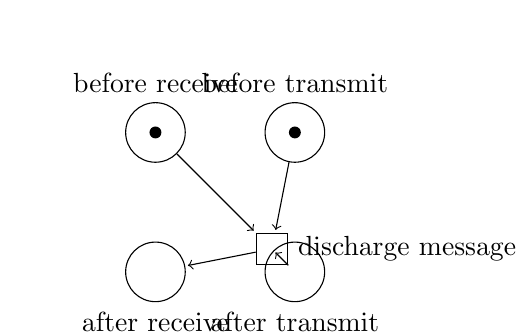
\begin{tikzpicture}
  \node[place,tokens=1,label=above:{before receive}] (beforeRx) {};
  \node[place,tokens=1,right = of beforeRx, label=above:{before transmit}] (beforeTx) {};
  \node[place,tokens=0,below=of beforeRx, label=below:{after receive}] (afterRx) {};
  \node[place,tokens=0,below=of beforeTx, label=below:{after transmit}] (afterTx) {};
  \node[transition,below right=of beforeRx, label=right:{discharge message}] (trans) {}
  edge [pre] (beforeRx)
  edge [pre] (beforeTx)
  edge [post] (afterRx)
  edge [post] (afterTx);
\end{tikzpicture}

Discharging a message here means copying the relevant bits of state from the transmitting thread's local state into the receiving thread's local state.
A message can be discharged if there is one thread willing to send it and one thread willing to receive it.
While the message is being discharged the two threads are effectively merged, with only one thread actually executing the message side effects.
Once the message is finished the two threads separate again and continue to execute independently.

A thread is only willing to receive a message if the message would pass the thread's message filter.
This has two parts:

\begin{itemize}
\item
  The message must have the correct message ID.
  This simply means that the send and receive parts of the message operation must be trying to enforce the same happens-before edge.
\item
  The message must pass the receiving thread's message receive filter.
  This filter consists of all of the side-conditions present in the crash enforcement plan which will become evaluatable once the message has been received.
\end{itemize}

However, in a real implementation, the threads are not pre-specified, and most of the complexity of the message algorithm lies in determining them.
When the plan demands that a message be sent or received, one side can be determined trivially, but the other must be discovered.
For a receive operation, the algorithm to do so in the abstract semantics looks like so:

\begin{algorithmic}[1]
  \IF {$l$ has a bound thread}
    \IF {The bound thread does not have an outgoing message}
      \STATE {Wait for it to send one}
    \ENDIF
    \IF {The bound thread has an outgoing message and it passes the message filter}
      \STATE {Discharge the message}
    \ELSE
      \STATE {$l$ has failed; remove it from the active set}
    \ENDIF
  \ELSE
    \STATE {Examine the set of outstanding unbound message sends and collect all of the ones which pass the message filter into $s$}
    \STATE {Extend $s$ with $\bot$}
    \STATE {Choose $s'$ non-deterministically from $s$}
    \IF {$s\prime = \bot$}
      \STATE {Register $l$ as a receiver of unbound messages}
      \STATE {Wait for the delay specified in this receive operation}
      \STATE {Unregister $l$ as a receiver of unbound messages}
      \STATE {Collect all of the unbound sends which pass the filter which started while we were waiting into $s$}
      \STATE {Select $s'$ non-deterministically from $s$}
    \ENDIF
    \STATE {Discharge $s'$}
  \ENDIF
\end{algorithmic}

The send operation is symmetric:

\begin{algorithmic}[1]
  \IF {$l$ has a bound thread}
    \IF {The bound thread is attempting to receive a message}
      \STATE {Wait for it to start receiving}
    \ENDIF
    \IF {The bound thread is receiving a message and this message would pass its filter}
      \STATE {Discharge the message}
    \ELSE
      \STATE {$l$ has failed; remove it from the active set}
    \ENDIF
  \ELSE
    \STATE {Examine the set of outstanding unbound message receives and collect all of the ones whose filters this message would pass into $s$}
    \STATE {Extend $s$ with $\bot$}
    \STATE {Choose $s'$ non-deterministically from $s$}
    \IF {$s' = \bot$}
      \STATE {Register $l$ as a sender of unbound messages}
      \STATE {Wait for the delay specified in this receive operation}
      \STATE {Unregister $l$ as a sender of unbound messages}
      \STATE {Collect all of the unbound receives whose filters this message would pass which started while we were waiting into $s$}
      \STATE {Select $s'$ non-deterministically from $s$}
    \ENDIF
    \STATE {Discharge $s'$}
  \ENDIF
\end{algorithmic}

As shown in figure ..., each message operation effectively defines an interval in time, and a send and receive match up if these windows overlap.
The behaviour when $s' = \bot$ is perhaps somewhat surprising: the thread waits a little while and then selects a peer thread to discharge the message with non-deterministically.
Meanwhile, all of the other threads are simultaneously performing similar non-deterministic choices.
The use of look-ahead nondeterminism means that all of the threads will make these selections in a mutually compatible way, so that there is no danger of A attempting to discharge its message with B while B discharges with C.
The actual implementation must resolve these constraints much more carefully, and is discussed in detail later.

Note that the message receive filter is evaluated as the message is being discharged, while the two threads are merged.
It is possible to imagine an alternative implementation in which the filter is instead evaluated locally in the receiver after the discharge operation is complete.
This would reduce the size of the synchronised section and so would appear, on the face of it, to offer greater parallelism, and hence potentially better performance.
Unfortunately, it does not work.
To illustrate the problem, consider again the example shown in figure \todo{...}.
One thread modifies a shared structure while another thread reads it, and the program will crash if the two threads happen to be operating on the same structure at the same time.
Suppose that the read thread runs far more often than the write one and that there are many instances of the structure.
The timeout balancing logic will quickly reduce the delay on the read side's first message send to zero and increase the delay on the write side's first message receive to compensate.
Now, when the write thread does run, it will stop just before \verb|l9| waiting for a matching read thread to arrive.
By hypothesis, many such threads will arrive, as the read thread runs more often than the write one.
In the alternative design, the read thread cannot evaluate the write thread's receive filter, and so every read thread will attempt to bind to the write thread, forcing the write thread to be duplicated many times.
Because of timeout rebalancing, the read thread will proceed from \verb|l2| immediately and quickly reach \verb|l5|, where it has to receive a message from \verb|l9|.
At this point, there are two possible outcomes:

\begin{itemize}
\item
  The thread is delayed at \verb|l5| waiting for the message from \verb|l9|.
  The write thread is still waiting in case any other threads reach \verb|l2| and attempt to synchronise with it, and so this might potentially be a rather long delay.
  Since the read thread runs far more often than the write thread, this will have a very large performance impact.
  Worse, it will probably be pointless: there, by hypothesis, a large number of instances of the structure which is being examined, and so, with high probability, the write thread will be modifying a different one.
  When the write thread does finally escape from its receive delay and evaluate its receive filter it will discover that the filter fails, and so the write thread will exit.
  The read thread will then discover that its bound thread has exited and be forced to exit as well.
  The crash enforcement plan will therefore not complete and the bug is highly unlikely to reproduce.
  
  Even worse, the performance hit might mean that the read thread will run far less frequently, further reducing the likelihood of the bug reproducing.
  In extreme cases, the attempt at enforcing a crash might actually make the bug less likely to reproduce in unit time.
\item
  The thread is not delayed at \verb|l5|.
  It never receives the message from \verb|l9| and must therefore exit without completing the plan, so is unlikely to reproduce the bug.
  The write thread's high-level interpreter will then accumulate a collection of low-level threads which have bound to exited read threads and which will themselves immediately exit.
\end{itemize}

Neither outcome helps to reproduce the target bug.

By contrast, in the scheme used by SLI, the read thread is able to evaluate the write thread's message receive filter at \verb|l2|.
It will therefore only bind to write threads which modify the structure which it is reading.
That means that the thread can be delayed a relatively long time at \verb|l5| without fear of apocalyptic performance damage, and so the bug will reproduce relatively easily.

\subsubsection{Discuss the timeout balancing bit}

Selecting the size of the various timeouts is important for determining the likelihood of reproducing a bug and the overheads of enforcing the patch.
SLI does so primarily dynamically, in response to the program's observed behaviour.

\subsubsection{Implementing non-deterministic choice in the Succ phase}

It might be that an instruction has several possible successors in the control flow graph in the crash execution plan, and in that case the interpreter must choose one of these successors using look-ahead non-determinism.
This cannot be implemented in any physically-realisable system, as it is non-causal, and so SLI must emulate it.
SLI uses a power-set construction to do so.
Rather than operating a single interpreter context, the actual implementation maintains a set of low-level interpreter contexts, which roughly follow the abstract semantics given above, and interprets them all in lock-step parallelism.
When one of these low-level interpreters needs to perform a non-deterministic choice between $n$ possible values, the high-level interpreter creates $n$ successor low-level interpreter states, one corresponding to each possible outcome of the choice, and inserts all of them into its current-state set.
They are then interpreted in parallel until enough information is available to resolve the earlier choice, at which point all but one of the threads will exit and the interpreter can revert to single-threaded execution.
If a thread is bound when it performs a non-deterministic choice then its bound thread must also be duplicated, to ensure that the new thread has something to bind to.

One subtlety here is that the original program's underlying instruction can only be retired once, and so the high-level interpreter must ensure that all low-level interpreters arrive at that point in the execution cycle at the same time.
SLI actually enforces a slightly stronger constraint, which is that every low-level interpreter in a given high-level interpreter must be at the same phase in the instruction execution cycle.
The only phases for which this is difficult are the message send and receive phases, which are discussed in more detail in the next section.

\subsubsection{Concrete implementations of message send and receive}

The message receive operation looks like this:

\begin{algorithmic}[1]
  \STATE {$lls \gets $ the set of currently-active low-level interpreter states}
  \STATE {$newLls \gets $ an empty set of low-level interpreter states}
  \FORALL {$l$ in currently-active low-level interpreter states}
    \IF {$l$ does not receive any messages}
      \STATE {Move $l$ from $lls$ to $newLls$ without changing it}
    \ELSIF {$l$ has a bound thread}
      \IF {$l$'s bound thread has exited}
        \STATE {$l$ exits as well; remove it from $lls$ without adding it to $newLls$}
      \ELSIF {$l$'s bound thread has an outgoing message}
        \IF {The bound thread's outgoing message passes the message filter}
          \STATE {Copy stashed values from the sending low-level interpreter's state to the receiving one}
          \STATE {Move $l$ from $lls$ to $newLls$}
        \ELSE
          \STATE {$l$ exits; remove it from $lls$}
        \ENDIF
      \ELSE
        \STATE {} \COMMENT {Wait for a the bound thread to send a message}
      \ENDIF
    \ELSE
      \STATE {} \COMMENT{Unbound receive}
      \FORALL {$s$ registered unbound senders}
        \IF {$s$'s outgoing message passes the message filter}
          \STATE {$l' \gets $ duplicate $l$}
          \STATE {$s' \gets $ duplicate $s$}
          \STATE {Copy stashed values from $s'$'s state to $l'$'s}
          \STATE {Bind $l'$ and $s'$ together}
          \STATE {Insert $l'$ into $newLls$}
          \STATE {Insert $s'$ into $s$'s high-level interpreter's active low-level interpreter list}
        \ENDIF
      \ENDFOR
      \STATE {Register $l$ as an unbound receiver}
    \ENDIF
  \ENDFOR

  \IF {$lls$ is empty}
    \RETURN
  \ENDIF

  \STATE {$end \gets now() + bound\_delay$}
  \IF {There is a minimum delay}
    \STATE {Release lock}
    \STATE {Sleep for the minimum delay}
    \STATE {Acquire lock}
  \ENDIF

  \WHILE {There are bound receives in $lls$ and $now() < end$}
    \STATE {Release lock}
    \STATE {Wait for some bound receive to complete, or for the current time to pass $end$}
    \STATE {Acquire lock}
    \FORALL {$l$ performing bound receives in $lls$}
      \IF {$l$'s bound thread has exited}
        \STATE {Remove $l$ from $lls$}
        \STATE {$l$ exits}
      \ELSIF {$l$'s receiving-bound-message flag is clear}
        \STATE {Remove $l$ from $lls$}
        \STATE {Add $l$ to $newLls$}
      \ELSE
        \STATE Continue waiting
      \ENDIF
    \ENDFOR
  \ENDWHILE

  \FORALL {$l$ in $lls$}
    \IF {$l$ is registered as an unbound receiver}
      \STATE {Unregister $l$ as an unbound receiver}
    \ENDIF
    \IF {$l$ was attempting a bound receive and the bound thread hasn't sent any messages}
      \STATE {Exit $l$}
    \ELSIF {$l$ is unbound}
      \STATE {The thread must have been attempting an unbound receive which failed, so exit $l$}
    \ELSE
      \STATE {} \COMMENT {Receive succeeded}
      \STATE {Add $l$ to $newLls$}
    \ENDIF
  \ENDFOR

  \STATE {Set high-level interpreters set of currently-active low-level interpreters to $newLls$}
\end{algorithmic}

The send algorithm is very similar:

\begin{algorithmic}[1]
  \STATE {$lls \gets $ the set of currently-active low-level interpreter states}
  \STATE {$newLls \gets $ an empty set of low-level interpreter states}
  \FORALL {$s$ in currently-active low-level interpreter states}
    \IF {$s$ does not send a message}
      \STATE {Move $l$ from $lls$ to $newLls$ without changing it}
    \ELSIF {$s$ has a bound thread}
      \IF {$s$'s bound thread has exited}
        \STATE {$s$ exits as well; remove it from $lls$ without adding it to $newLls$}
      \ELSIF {$s$'s bound thread is waiting to receive a message}
        \IF {$s$'s outgoing message passes the message filter}
          \STATE {Copy stashed values from the sending low-level interpreter's state to the receiving one}
          \STATE {Move $s$ from $lls$ to $newLls$}
          \STATE {Clear the bound thread's receiving-bound-message flag}
        \ELSE
          \STATE {$s$ exits; remove it from $lls$}
        \ENDIF
      \ELSE
        \STATE {} \COMMENT {Wait for a the bound thread to be ready to receive a message}
      \ENDIF
    \ELSE
      \STATE {} \COMMENT{Unbound send}
      \FORALL {$l$ registered unbound receivers}
        \IF {The outgoing message passes $l$'s message filter}
          \STATE {$l' \gets $ duplicate $l$}
          \STATE {$s' \gets $ duplicate $s$}
          \STATE {Copy stashed values from $s'$'s state to $l'$'s}
          \STATE {Bind $l'$ and $s'$ together}
          \STATE {Insert $s'$ into $newLls$}
          \STATE {Insert $l'$ into $l$'s high-level interpreter's active low-level interpreter list}
        \ENDIF
      \ENDFOR
      \STATE {Register $s$ as an unbound sender}
    \ENDIF
  \ENDFOR

  \IF {$lls$ is empty}
    \RETURN
  \ENDIF

  \STATE {$end \gets now() + bound\_delay$}
  \IF {There is a minimum delay}
    \STATE {Release lock}
    \STATE {Sleep for the minimum delay}
    \STATE {Acquire lock}
  \ENDIF

  \WHILE {There are bound sends in $lls$ and $now() < end$}
    \STATE {Release lock}
    \STATE {Wait for some bound send to complete, or for the current time to pass $end$}
    \STATE {Acquire lock}
    \FORALL {$s$ performing bound sends in $lls$}
      \IF {$s$'s bound thread has exited}
        \STATE {Remove $s$ from $lls$}
        \STATE {$s$ exits}
      \ELSIF {$s$'s sending-bound-message flag is clear}
        \STATE {Remove $s$ from $lls$}
        \STATE {Add $s$ to $newLls$}
      \ELSE
        \STATE Continue waiting
      \ENDIF
    \ENDFOR
  \ENDWHILE

  \FORALL {$s$ in $lls$}
    \IF {$s$ is registered as an unbound sender}
      \STATE {Unregister $s$ as an unbound sender}
    \ENDIF
    \IF {$s$ was attempting a bound send and the bound thread hasn't tried to receive any messages}
      \STATE {Exit $s$}
    \ELSIF {$s$ is unbound}
      \STATE {The thread must have been attempting an unbound send which failed, so exit $s$}
    \ELSE
      \STATE {} \COMMENT {Send succeeded}
      \STATE {Add $s$ to $newLls$}
    \ENDIF
  \ENDFOR

  \STATE {Set high-level interpreters set of currently-active low-level interpreters to $newLls$}
\end{algorithmic}

One further optimisation, not shown here, avoids redundantly duplicating low-level interpreter contexts in the common case that a message operation is discharged precisely once.

\todo{This is probably not the best way of presenting those
  algorithms.}

\todo{Discuss setting minimum delays here}

\subsubsection{The await-bound-thread-exit state}

When a thread completes its plan, it is sometimes useful for it to wait for its bound thread to exit before proceeding.
This is because the crash summary from which the plan is generated does not have complete information on the structure of the program.
If the last edge in a happens-before graph is from memory access A to memory access B, that generally means that A is a store and B is a load and B must load the value stored by A.
That means that, not only must B happen after A, but B must happen before any other writes to the memory location modified by A.
If there were other stores to that location in the crash summary then the happens-before graph would include additional edges to ensure that that happens, but if there are stores outside of the summary then it will not.
For instance, suppose that the write thread looks like this:

\begin{verbatim}
while (1) {
l1:  *x = 5;
l2:  *x = 7;
     <something_complicated>
}
\end{verbatim}

And the read thread looks like this:

\begin{verbatim}
l3: a = *x;
l4: b = *x;
    crash if a != b;
\end{verbatim}

This program is clearly buggy.
One way of reproducing this bug would be to interleave instructions as \verb|l1|, \verb|l3|, \verb|l2|, \verb|l4|.
SLI will discover this interleaving as the happens-before graph show in figure \todo{...}.
The algorithm described so far will be sufficient to enforce this graph (assuming that the two fragments of code shown can actually execute in parallel).
This is not, however, sufficient to cause the program to crash, because the generated happens-before graph is incomplete: it misses the edge from \verb|l4| to \verb|l1| in the next iteration of the loop.
If the loop completes and reaches the store at \verb|l1| before the load \verb|l4| completes then the bug will not reproduce even though the happens-before graph was successfully enforced.
Any scheme with an analysis horizon based on a simple instruction count will suffer from a similar problem, but this is particularly serious for SLI, because the delays inserted are in almost precisely the right place to maximise the chance of this kind of bug-hiding race.
Returning to the example, SLI's crash enforcement plan will include a delay after \verb|l1| (to implement the \verb|l1| to \verb|l3| happens-before edge), and this delay will be large relative to a short sequence of normal instructions, and so the bug will be hidden completely provided that the delay to wake up the read thread after the final edge is greater than the time taken to execute \verb|<something_complicated>|.
This is perfectly plausible, given that \verb|<something_complicated>| only needs to be a few dozen instructions to exceed SLI's analysis window.
This bug will therefore never reproduce under SLI's crash enforcer, even when the happens-before graph is enforced perfectly.
The fix is simple: have the store thread delay slightly after completing its final message send operation, until the read thread also completes its crash enforcement plan.
This ensures that activity beyond the analysis horizon cannot prevent bug reproduction, and, because it only happens when the plan is mostly complete, and hence happens very rarely, it has very low performance overhead.

\begin{tikzpicture}
\node[CfgInstr] (l1) {l1};
\node[CfgInstr, below = of l1] (l2) {l2};
\node[CfgInstr, right = of l1] (l3) {l3};
\node[CfgInstr, below = of l3] (l4) {l4};
\draw[->] (l1) -- (l2);
\draw[->] (l3) -- (l4);
\draw[->,happensBeforeEdge] (l1) -- (l3);
\draw[->,happensBeforeEdge] (l3) -- (l2);
\draw[->,happensBeforeEdge] (l2) -- (l4);
\end{tikzpicture}


\subsubsection{Compiling the plan}

\todo{Implementation of this is currently massively broken; need to
  decide whether I'm going to fix it or just use a slightly older
  version.}

In addition to a plan interpreter, SLI also includes a plan compiler, which combines the plan with the program's original machine code to produce a modified version of the program which performs the necessary enforcement actions without needing an interpreter.
The intent here is to reduce the overhead of the interpreter in the case where SLI is investigating many bugs most of which do not exist.
Making this practical requires several simplifications to the semantics:

\begin{itemize}
\item
  The number of physical program threads operating in the plan is limited.
  In particular, it is assumed that only one program thread will be executing the read side of the plan at any time, and likewise only one thread will be executing the write side.
\item
  The message semantics are simplified: messages are sent asynchronously, with a delay only on the read side, and must be ``cancelled'' when the relevant thread exits.
  This has two important implications: first, that a message send can never fail and, second, the something must keep track of what messages a given thread currently has outstanding.
  Combined with the first simplification, it also means that at most one instance of any given message can be outstanding at any one time, and so it is easy to place the relevant information in a global structure without needing any dynamic memory allocation.
\item
  High-level interpreter contexts only ever access the state of their own low-level interpreters.
  This has two important implications:

  \begin{itemize}
  \item
    Remote low-level interpreters are never duplicated during message operations.
    If the normal semantics would require an interpreter to be duplicated then the local message operation fails.
  \item
    The receive message filter can only be executed by the receiving thread after receiving a message.
  \end{itemize}
\item
  When a low-level interpreter is duplicated due to a non-deterministic choice in the Succ phase the low-level state's stash table is not duplicated.
  Instead, all low-level interpreters in a given high-level interpreter share a single stash table.
\end{itemize}

The result is a system with lower run-time overheads, but also a lower probability of reproducing interesting bugs.
It has a much larger I-cache footprint but a smaller D-cache one\editorial{Not sure where I'm going with that, although it is true and kind of interesting}.

I now briefly outline the implementation of this compiler.
The core idea is to compile the CFG in the enforcement plan into a state machine.
This state machine consists of a large number of smaller intra-instruction state machines, as illustrated in figure~\todo{...}, each of which models a single instruction in the original program.
The label on each state is itself a set of low-level labels which consist of a four-tuple of the plan thread which is executing, a reference to the plan CFG node, a set of messages which have been sent by the thread, and the phase of the intra-instruction state machine.
Each state is compiled to a small fragment of machine code (which might be empty, if this instruction does not have an relevant annotation in the plan) plus a set of relocations specifying the fragment's relationships to the other states.
Once every state has been compiled these relocations can be discharged and the fragments concatenated together to form the final patch.

I now discuss the details of each phase of the intra-instruction machine:

\begin{itemize}
\item[RecvMsg]
  Examine the set of CFG nodes which are active in the current state and determine whether the plan requires any of them to receive messages.
  If so, emit code to examine the global outstanding-message structures to see whether of the desired messages are currently outstanding.
  If there are, receive precisely that message.
  Any other message receive operations are considered to have failed and the relevant CFG nodes removed from the current state label.
  If no message sends are currently outstanding then the physical thread is delayed until either one is available or some timeout is reached.
  If a message becomes available then it is received, and otherwise all receives fail and all receiving CFG nodes are removed from the label.
  Note that this does not necessarily mean that the state label will become empty\footnote{Although that is the common case.} as there may be some CFG nodes which do not need to receive messages.

  Once a message is received its content is simply copied from the global message area into the local thread's stash area.
\item[OrigInstr]
  Store any generated values into simulation slots and issue the original instruction.
  There are three main cases to consider here:

  \begin{itemize}
  \item
    Simple memory loads.
    If the instruction is of the form \verb|LOAD *location -> register|, and the value loaded is to be saved, then it is sufficient to just copy \verb|register| into the simulation slot after the original instruction has completed.
  \item
    Compound memory loads.
    Instructions which load from memory but are not themselves simple loads are more difficult to handle.
    For concreteness, suppose that the instruction is \verb|CMP 76,*loc1|, and the annotation requires us to save the value loaded.
    The instruction loads from \verb|*loc1| but does not leave the result in any locations which we can easily access.
    It would be possible to solve this problem by adding another load of \verb|*loc1|, but that would run the risk of a store in a remote thread modifying \verb|*loc1| between the two loads, leading to very confusing results.
    SLI instead solves this problem by rewriting the instruction to this:

\begin{verbatim}
LOAD *loc1 -> reg1
STORE reg1 -> simslot
CMP 76, reg1
\end{verbatim}

    This exposes the loaded value to the instrumentation framework, allowing it to be stored to the simulation slot as desired.

    Instructions which modify memory in-place, such as \verb|ADD 1 + *loc1 -> *loc1|, pose a similar problem and can be solved in the same way, provided that they do not have a \verb|LOCK| prefix.
    \verb|LOCK|ed instructions are more complex, as separating the load and store phases into separate instructions would violate the semantics of the program and might introduce new bugs.
    SLI solves this problem using a \verb|CMPXCHG| loop.
    For instance, the instruction \verb|LOCK ADD 1 + *loc1 -> *loc1| would be converted to this machine code fragment:

\begin{verbatim}
1: LOAD *loc1 -> reg1
ADD 1 + reg1 -> reg2
LOCK CMPXCHG *loc1, reg1 -> reg2
if_cmpxchg_failed goto l1
STORE reg1 -> simslot
\end{verbatim}

    The \verb|CMPXCHG| instruction here is supposed to be an invented syntax for the x86 machine code instruction which atomically compares \verb|*loc1| to \verb|reg1| and, if they are equal, sets \verb|*loc1| to \verb|reg2|.
    This allows SLI to expose the value of the implicit load while preserving the \verb|LOCK| semantics of the original instruction.
  \item
    Branch instructions are deferred to the FindSucc state.
  \end{itemize}
  
\item[SendMsg]
  Send any outgoing messages.
  This amounts to simply copying the message payload into the global message area, setting a global flag to indicate that the message is currently outstanding, and adding the message ID to the state label's set of sent messages.
  This always succeeds and advances to the FindSucc state.

\item[ExitThread]
  When a low-level thread exits it is necessary to cancel any messages which it has sent.
  The compiler takes the union of all of the sent-messages sets in its low-level, removes the thread which is to exit, and then takes the union again.
  Any messages present in the first set but not the second need to be cancelled by setting the relevant global message-outstanding flag to zero.
  The compiler will then either exit the patch, if the last low-level thread has exited, or resume the intra-instruction state machine at an appropriate place.
\end{itemize}


\begin{tikzpicture}
\node[flowChartState] (RecvMsg) {RecvMsg};
\node[flowChartState,above left = of RecvMsg] (StartThread) {StartThread};
\node[flowChartState,above right = of RecvMsg] (CheckForThreadStart) {CheckForThreadStart};
\node[flowChartState, below = of RecvMsg] (OrigInstr) {OrigInstr};
\node[flowChartState, below = of OrigInstr] (VerfCond) {VerfCond};
\node[flowChartState, below = of VerfCond] (SendMsg) {SendMsg};
\node[flowChartState, below = of SendMsg] (FindSucc) {FindSucc};
\node[flowChartState, right = of VerfCond] (CondFail) {CondFail};
\node[flowChartState, right = of CondFail] (Exit) {Exit};
\node[flowChartState, left = of RecvMsg] (RecvdMsg) {RecvdMsg};
\draw[->] (CheckForThreadStart) -- (RecvMsg) -- (OrigInstr) -- (VerfCond) -- (SendMsg) -- (FindSucc);
\draw[->] (StartThread) to [bend right=10] (CheckForThreadStart);
\draw[->] (CheckForThreadStart) to [bend right=10] (StartThread);
\draw[->,dashed] (FindSucc.east) to [bend right=75] (CheckForThreadStart.east);
\draw[->] (RecvMsg) -- (RecvdMsg) -- (OrigInstr);
\draw[->] (RecvMsg) -- (Exit);
\draw[->] (VerfCond) -- (CondFail) -- (Exit);
\draw[->] (FindSucc) -- (Exit);
\end{tikzpicture}

  

\subsubsection{Compiling entry point stubs}
\label{sect:find_bugs:compile_entry_points}

\todo{Good Lord, this is completely incomprehensible.}

The entry points of the crash enforcement plan are given as mappings from call stacks to CFG nodes.
The program must be patched so that it transfers control to the interpreter whenever the call stack matches up with one of these entry-point call stacks.
This is a multi-step process:

\begin{itemize}
\item
  The last pointer in the call stack is a raw instruction pointer.
  The relevant instruction is patched into a jump into the interpreter trampoline.
\item
  The interpreter trampoline transitions to a different stack, saves the client program's register state, and starts the main interpreter.
\item
  The main interpreter then examines the program's stack to determine whether it matches up with the entry-point stack.
  If it does then a new high-level interpreter state is created and interpretation starts.
  Otherwise, the interpreter exits back to the original program (possibly after emulating enough instructions to avoid returning into the middle of the new jump instruction).
\end{itemize}

The last point is more subtle than it might appear, as the interpreter must be able to find arbitrary return addresses on the program's stack, and this is difficult if the program is compiled without frame pointers or debug symbols.
SLI uses a static analysis, performed when generating the crash enforcement plan, to solve this problem.
The static analyses already described are sufficient to determine the entry point of the function containing a given RIP, and so it is easy to perform a simple abstract interpretation forwards from that point to the given RIP and hence find the number of bytes which the function will push onto the stack on the way\footnote{This is generally fixed for all possible paths}.
The first entry in the call stack is trivially true because of the way the jumps are patched in.
The second one is the return address of the current function, which can be found using that offset.
The third one is the return address of the calling function, and the offset there is just the previous offset plus the offset in the calling function.
In this way all necessary offsets can be found and the entry-point stack checked completely.

\subsubsection{Run-time considerations}

Recovery from spurious segfaults in the patch due to e.g. LD operations.

\subsection{Comparison to schedule memoisation}
\subsection{Comparison to STM block inference stuff}



\chapter{Other modes of operation}
\section{Fixing bugs}

\subsection{Using global locks}
\label{sect:fix_global_lock}

In addition to finding bugs, SLI can also be used to fix them in a
largely automated fashion.  The basic approach here is to binary patch
the program to introduce a new global lock covering the program's
relevant instructions, preventing them from executing in parallel and
hence preventing the bug from occurring (assuming that the relevant
instructions have been correctly identified).  The relevant
instructions are duplicated into a binary patch, unrolling loops and
tracing across function boundaries in a way which reflects the
function inlining and loop unrolling performed during the initial CFG
generation phase, and the duplicates modified to acquire and release
the lock at appropriate points.  The original program is then patched
branch to the duplicates when necessary.

The first step in producing such a fix is correctly identifying the
instructions which must be included in the critical sections.  These
will be roughly a subset of the instructions involved in the
control-flow graphs associated with \StateMachines; a subset because
some instructions in the CFG do not need to be protected, and roughly
because some instructions not in the CFG will also be included in the
critical section.

As an example of the former, consider a program like this:

\begin{verbatim}
read_side() {
    ptr = complicated_local_calculation();
    dptr = *ptr;
    if (dptr != NULL) {
       dptr = *ptr;
       *dptr = 5;
    }
}
write_side() {
    ptr = complicated_local_calculation();
    *ptr = NULL;
}
\end{verbatim}

Here, the read thread computes some pointer using entirely local
operations, loads from it once and then, if the result is
non-\verb|NULL|, loads from it again and uses the resulting pointer.
Meanwhile, the store thread sets a potentially coincident memory
location to \verb|NULL|.  The read thread clearly has a potential
time-of-check, time-of-use race bug.  The \StateMachines generated by
SLI will include the buggy code itself but might also include part or
all of \verb|complicated_local_calculation()| and a side-condition
which requires the two pointers to match up.  This extra information
is useful when analysing the bug (\needCite) or when attempting to
reproduce it (\needCite) but cannot be used by this kind of
instruction-level fix\footnote{But see future work section~\needCite
  for a possible alternative scheme which would make use of it.}, so
including it in the fix is unhelpful and would tend to lead to
unnecessarily large critical sections.  The fix generating process
must therefore select a useful subset of the instructions in the
control-flow graph.

The approach taken here is simple:

\begin{itemize}
\item
  Reduce the verification condition from the bug summary until it
  contains only happens-before edges.  These entirely capture the
  instruction-interleaving parts of the bug to be fixed, and, since
  instruction-interleaving is the only thing which can be influenced
  by this type of patch, the resulting condition contains all of the
  useful information in the condition.
\item
  Identify all of the CFG nodes which are mentioned in one of those
  happens-before edges.
\item
  Trim the CFG such that every path starts and ends in one of those
  mentioned nodes.  All such paths will be included in a critical
  section, and so no such paths will be permitted to execute in
  parallel.
\end{itemize}

In this way the CFG is restricted to just those instructions which are
involved in the interleaving which is to be prevented.

Note that this is not guaranteed to produce an optimal selection of
critical sections, in the sense that sections can sometimes be larger
than is strictly necessary.  Consider, for example, a program with the
same read side as the previous example but a write side in which the
pointer is assigned to twice:

\begin{verbatim}
write_side() {
    ptr = complicated_local_calculation();
    *ptr = NULL;
    *ptr = NULL;
}
\end{verbatim}
    
There are now two obvious ways of protecting this program:

\begin{itemize}
\item
  Place both loads in the read side in a single critical section and
  both stores in the write side in another one.
\item
  Place both loads in the read side in a single critical section, but
  give each store in the write side its own critical section.  In
  other words, drop and re-acquire the lock in between the two stores.
\end{itemize}

Both approaches correctly eliminate the bug, but they will have
different performance characteristics.  In particular, dropping and
re-acquiring the lock reduces the size of the critical section, which
might improve concurrency and reduce starvation, but imposes higher
overheads due to the greater number of lock operations.  In principle
the happens-before graph implicit in the verification condition
contains enough information to determine whether dropping the lock is
safe, but, in this mode, SLI does not make use of this information,
and always uses the former strategy\footnote{But
  see~\ref{sect:fix_from_drs} for a mode in which it can use the other
  approach.}.

Once the relevant fragment of CFG has been identified, entry point
stubs must be generated and the program patched to branch to them at
appropriate points.  There are two main complications here:

\begin{itemize}
\item
  Instructions on x86 are not all the same size, and, in particular, a
  branch instruction is larger than some of the instructions which
  need to be patched.  This means that replacing an instruction with a
  branch to a patch entry point stub might clobber the following
  instruction; if there are any branches to that instruction from
  anywhere else in the program then the results are unlikely to be
  helpful.
\item
  The control-flow graphs used by SLI can cross function boundaries,
  and in particular are sometimes only valid in a particular function
  call context.  The patch must therefore check that the stack matches
  before attempting to run the CFGs.  Note, in particular, that
  whereas stack context checking is a performance optimisation when
  trying to trigger bugs it is necessary for correctness when trying
  to prevent them.
\end{itemize}

SLI solves the first problem by expanding the critical sections
backwards so that they do not start on dangerous instructions.  The
early static analysis passes discover all of the branches within the
program, and so can detect when inserting a branch would cause a
dangerous clobber, and in that case it simply expands the critical
section to include the instruction's predecessors\footnote{This might,
  of course, mean that the critical section has multiple entry points;
  that is not a problem.}.  The process then iterates until a safe
instruction is found\editorial{What if no safe instruction is found
  e.g. a loop with no suitable instructions in?  That does actually
  work, but, thinking about it, I'm not entirely certain why; should
  check that.}.  One complication here is branches from libraries into
the main program, which will not be detected by the static analysis.
Fortunately, they are detected by the dynamic analysis, and so this is
not a problem\editorial{Assuming that the dynamic analysis is
  complete, which is kind of a big assumption.  Saying that we miss
  some bugs when the analysis is incomplete is one thing; saying that
  we introduce more is a bit more of a big deal.  Probably need to say
  a bit more about that.}.

This problem was also tackled by the AutoPaG project, and the solution
they developed is similar. \todo{Similar but not the same.  They use a
  dominator-based scheme, and hence avoid needing the global branch
  information but can end up with much larger patches and a higher
  risk of deadlocks/starvation problems.  The original version of SLI
  used basically the same algorithm (although I did it first); should
  probably explain why I had to switch.}

The second problem, checking function call contexts, is much simpler,
and SLI solves it by simply emitting machine code to perform the
appropriate checks (using a stack layout derived in the same way as in
\S~\ref{sect:find_bugs:compile_entry_points}) and branch to an
appropriate place in the patch (or return to the original program if
there is none).  One subtlety here is that the original instruction
will have been replaced by a branch, and so returning to it directly
is unlikely to be effective, and so SLI copies the branch into the
patch (and possibly also a small number of clobbered instructions, if
necessary) and executes them from the patch before returning, without
holding the patch lock.\editorial{Rewrite the whole damn paragraph.}

An alternative approach would be to take control of the program using
debug breakpoints rather than jump instructions.  These are either a
single byte (for the \verb|int3| instruction) or no bytes at all (for
debug registers), and so avoid the instruction clobbering problem.
This would work, but would have a couple of important disadvantages:

\begin{itemize}
\item
  Debug breakpoints are far slower than branches.  This might be
  important if the critical section is to be inserted on a
  particularly hot code path.
\item
  Using debug breakpoints in this way would interfere with any other
  debugger which the developer might want to use.  With a branch-style
  patch, standard debuggers work without modification for any part of
  the program which has not been patched, whereas a breakpoint-style
  patch requires extensive coordination between the debugger and the
  patch mechanism for either to work at all.
\item
  Breakpoint registers are of strictly limited number on most
  architectures (four, on x86).  This means that they can never
  provide a complete solution by themselves.
\item
  On most UNIX-type operating systems, including Linux and FreeBSD,
  catching debug breakpoints requires modifying the program's signal
  handling configuration, which requires some level of coordination
  with the program to be modified.  It would be possible to use an
  alternative API, but this would require kernel modifications,
  complicating the use of the generated patches\footnote{Branch-style
    patches also require modifying signal handling configurations in
    order to, for instance, provide a correct faulting instruction
    address in SIGSEGV register configurations.  However, very few
    programs actually require that information for correctness, and so
    it is not usually a major issue if the patch loses control of the
    signal handler to the main program.  In a breakpoint-style patch,
    losing control of the signal handler means, first, that the patch
    is never run, and so cannot hope to fix the bug, and, second, that
    the program receives spurious breakpoint events, which will often
    introduce additional erroneous behaviour.}.
\end{itemize}

SLI therefore generates predominantly branch-style patches.

\todo{I did implement a breakpoint-based scheme, so it might be
  interesting to actually include some numbers on their relative
  effectiveness.}

\subsection{Other ways of fixing the bugs}
\todo{I've come up with an algorithm for doing this using a message
  passing network, like we do for crash enforcement but with the
  delays in slightly different places, but I really don't have time to
  implement it.  It is kind of cool, though; I'd like to include it
  somewhere, even if it's just a future work-type thing.}

\todo{Might also be worth saying a few words about possibly fixing the
  bugs by using STM-like techniques?  I've not implemented any of
  them, either, but they are kind of interesting.  Probably worth a
  paragraph or two.}

\section{Fixing bugs from DRS logs}
\label{sect:fix_from_drs}
The simplest way to fix a bug is to start from a DRS log.
Given a log, identifying the thread and which is most responsible for a crash is generally straightforward.
If the crash is caused by dereferencing a bad pointer then the responsible thread is the one which dereferenced the pointer; if the crash is an assertion failure then the responsible thread is the one which called \verb|abort()| (or equivalent).
The log then makes it trivial to determine what instructions the responsible thread executed before it crashed, and a suffix of these can be compiled into a \StateMachine capturing the most relevant parts of the responsible thread's behaviour.

The log also makes it trivial to determine precisely which stores the read-side thread raced with, and so building a write-side \StateMachine is redundant.
Instead, the read-side \StateMachine is ``slid across'' the log, evaluating it at every step (subject to some typing constraints which ensure that the result is reasonable), and the resulting pattern of safe and unsafe regions converted directly into critical sections, without ever needing to generate an explicit write-side \StateMachines.

\subsection{Building the read-side \StateMachine}
\todo{This is gratuitously different from the non-DRS mode in an enormous number of places.  I should fix that.}

Working from a DRS log provides a lot of information which is not available in SLI's normal mode of operation.
This makes some parts of the algorithm redundant.
In particular, there is no need to generate large numbers of CFGs of fragments of the program which might be relevant, as we know precisely which instructions were executed leading up to the crash.
Instead, in this mode, SLI generates the \StateMachine directly from the log.
It starts with a small stub machine representing just the instruction which crashed and then expands it backwards, incorporating a single instruction from the log at a time.
For instance, suppose that the fragment of program to be investigated looked like this:

\begin{verbatim}
l1: mov $5, %rax
l2: mov (global1), %rbx
l3: mov (%rax + %rbx), %rcx
\end{verbatim}

and the program crashed due to dereferencing a bad pointer at \verb|l3|.
The initial stub \StateMachine will then be just:

\begin{verbatim}
if (BadPtr(rax + rbx)) crash(); else survive();
\end{verbatim}

Incorporating \verb|l2| will transform that to

\begin{verbatim}
LOAD (global1) -> rbx
if (BadPtr(rax + rbx)) crash(); else survive();
\end{verbatim}

Incorporating \verb|l1| will then produce the \StateMachine

\begin{verbatim}
COPY 5 -> rax
LOAD (global1) -> rbx
if (BadPtr(rax + rbx)) crash(); else survive();
\end{verbatim}

Which can be simplified in the usual way to produce

\begin{verbatim}
LOAD (global1) -> rbx
if (BadPtr(rbx)) crash(); else survive();
\end{verbatim}

And this can then be used in the rest of the analysis.

The major subtlety here lies in the handling of control flow, and the parts of the program which are not executed.
One possible approach would be to simply say that any changes to the control flow cause the bug to be avoided, but this is over-optimistic.
Consider, for instance, a program like this one:

\begin{verbatim}
ptr = global;
if (some_condition)
    idx = 1;
else
    idx = 2;
local = ptr[idx];
\end{verbatim}

This program loads a pointer to an array from a global variable and then loads some index in the array, with the index chosen depending on some condition.
Suppose that the race then causes the pointer in \verb|global1| to sometimes be bad, and that the reproduction of the bug was obtained while \verb|some_condition| holds.
The bug itself does not depend on \verb|some_condition|, but if one were to assume that any changes to control flow avoid the bug then SLI would not be able to show this.
This problem can only be avoided by exploring untaken branches, and SLI does so, for some (configurable) number of instructions.
If the control flow rejoins that which is represented in the DRS log then an appropriate branch is included from one part of the \StateMachine to another, and if it does not rejoin then a branch to the \verb|NoCrash| state is used instead.

One complication here is that a given static instruction might be represented multiple times in the DRS instruction trace, and hence multiple times in the \StateMachine, if the instruction is part of some loop.
This makes it ambiguous where the branch should branch to.
SLI solves this problem by taking the earliest instance of the instruction, and hence branching to the place in the \StateMachine nearest the root.
This helps to keep the loop structure of the program intact, subject to the unrolling implicit in the DRS log.

The example shown above might then turn into a \StateMachine something like this:

\begin{verbatim}
LOAD global1 -> ptr
if (some_condition) {
   COPY 1 -> idx1
} else {
   COPY 2 -> idx2
}
if (BadPtr(ptr + idx)) {
   crash();
} else {
   survive();
}
\end{verbatim}

The standard simplified will then transform that to this:

\begin{verbatim}
LOAD global1 -> ptr
if (BadPtr(ptr + (some_condition ? 1 : 2))) {
   crash();
} else {
   survive();
}
\end{verbatim}

SLI uses a rule that \verb|BadPtr(x + k)| is equivalent to \verb|BadPtr(x)| whenever \verb|k| is a small constant, and so correctly determines that the bug is independent of \verb|some_condition| in this case.

\todo{Discuss using more powerful bug definitions here e.g. Valgrind, invariant discovery, etc, by applying them to the log and then converting to stub machines, so that you can apply this to races which lead to bugs other than immediate bad pointer dereferences.}

\subsection{Requirements on the DRS}

\subsection{Finding remote critical regions}

The fixes generated by SLI rely on making the read-side \StateMachine operate as-if atomically and then ensuring that it does not execute in any states where doing so would lead to a crash.
In the normal mode of operation, the regions which would lead to a crash are determined by modelling the rest of the program as a set if write-side \StateMachines and then using symbolic execution, but it is possible to be more accurate\editorial{or possibly precise?} if a full DRS log is available.
Instead of the set of \StateMachines, the log itself can be used as a model for the rest of the program.
The idea here is that the log contains a sequence of possible states of the program, and contains all of the ones which are relevant to this particular way of reproducing the bug of interest.
SLI therefore slides the read-side \StateMachine over this log, evaluating it at every instruction, and hence classifies the log into ``safe'' and ``unsafe'' regions, and the transitions between these two types of region give the boundaries of the write-side critical regions.

As a minor optimisation, SLI only re-evaluates the \StateMachine if there has been a store to some memory location which is loaded by the \StateMachine.
This cannot affect the results in any way, but means that the \StateMachine does not have to be evaluated as often.

One important complication here is the presence of dynamically-allocated data structures.
SLI relies on being able to identify points in the program where these are allocated and released.
The loads in the read \StateMachine will correspond to specific load operations in the DRS log and SLI is then able to check which dynamic instance of structures those accesses access and will only evaluate the \StateMachine while all of the relevant structures remain live.

Once the log has been classified, the classification must be converted into realisable critical sections.
In other words, SLI must identify points in the program at which it must insert lock acquire operations and points where it must insert lock release operations.
Ideally, each unsafe region in the log would correspond to a single critical section, with a single acquire operation and a single release one.
This can fail in several ways:

\begin{itemize}
\item
  The start and end of the unsafe region might be in different threads, if, for instance, one thread violates an invariant and another thread then restores it.
  It is difficult to model a cross-thread operation as a critical section.
  SLI cannot prevent this kind of bug, and the unsafe region is simply ignored.
\item
  There might be non-trivial control flow between the start and end of an unsafe region within a single thread.
  In that case additional acquire and release operations must be inserted to ensure that locks are not leaked, double-acquired, or double-released.
\item
  The program might have additional synchronisation mechanisms which, when combined with the SLI-inferred synchronisation, lead to a deadlock.
\end{itemize}

These are discussed in more detail in \S~\ref{sect:fix_global_lock}.

\todo{This is in dire need of rewriting.}

Note that the definition of a dynamic structure is somewhat subtle here.
Most obviously, \verb|malloc| and \verb|free| represent boundaries in the lifespan of such structures (with \verb|malloc| being the start and \verb|free| being the end), but ``re-typing'' operations can also impose such boundaries.
The intent of the sliding procedure is to capture other operations which the program might perform on the data structures involved in the synchronisation bug, in the same way that write-side \StateMachines do in the non-DRS case.
In effect, the program's behaviour is constrained using a heuristic memory safety property, and this memory safety property must correspond reasonably closely to the program's actual structure.

The underlying hypothesis here is that the program has some kind of internal type system which constrains which operations will be performed on a given memory location.
This means that two pieces of code can only race if they have types which are in some sense compatible, so that they might access overlapping memory locations.
The combination of the read-side \StateMachine and the set of dynamic instances accessed by it defines, in a slightly ill-defined way, a set of types which the read side of the critical section might access.
SLI must then find some other operations on the same types to synchronise against, and this is the aim of the sliding procedure.
In order for this to work, the read \StateMachine must only be slid to places where the current types match up with the types for which it was derived.
SLI must therefore be able to identify points where the types of memory locations change.
This includes things like \verb|malloc| and \verb|free|, but is also likely to include things like program-specific memory allocators or object pools.
The precise set will depend on the program's type system, and so can only be sensibly modelled with assistance from the programmer.




\chapter{Analysis on \StateMachines}

\section{Alias analysis}
\subsection{Alias analysis and identification of thread-local accesses}
There are two major complications to optimising memory accesses:

\begin{itemize}
\item
  Alias analysis.
  Most memory-related optimisations rely on being able to tell whether two pointers alias with each other.
  This is impossible in the general case, but it is possible to develop some useful (sound and unsound) approximations.
  This is very similar to the problem of the same name faced by optimising compilers, except that optimising compilers generally have more information (e.g. type information).
\item
  Checking whether an access is thread-local.
  Most races are mediated through memory, and all of the races targeted by SLI will involve some memory-accessing component.
  Correctly handling races restricts the available space of optimisations, often substantially.
  For instance, if a machine stores to a location and then immediately loads from it again then it might be tempting to forward the stored expression to the load, but this is invalid if another thread might store to the same location in between the two accesses.
  This is a common cause of races, and one which can be easily handled by SLI-like techniques, and so it is important not to eliminate it at the machine simplification stage.
\end{itemize}

If a DRS log is available then this is generally trivial, as all of the necessary information will be present in the log\editorial{should really have a ref to the DRS section, which'll have more details.}.
Otherwise, SLI uses a combination of static and dynamic analyses to solve these problems.

\subsubsection{Dynamic analysis}

The most important technique used by SLI is a dynamic analysis which is used before starting static analysis to build a model of how the program behaves.
This attempts to classify the memory-accessing instructions in the program according to which other memory accesses they might alias with and whether the memory accesses appears to be private to that thread.
The result is an aliasing database which consists of a set of aliasing entries.
Each aliasing entry consists of a pair of sets of instructions, with one set containing loads and the other stores, with each instruction tagged with a bit saying whether the accessed memory was thread-local or possibly-shared.
The database is generated using a dynamic analysis implemented as a Valgrind skin.

\todo{Should really describe how the skin works.  Mostly just an engineering detail, though.}

\todo{The bit where we figure out whether a dynamic pointer is thread-private is kind of interesting, though.}

Given this database, it is generally possible to eliminate the vast majority of possibly-aliasing pairs quickly, which means that the aliasing problem becomes much simpler.
Of course, it is only correct if the dynamic execution completely captures every possible behaviour of the program.
This is a particular concern if the program is misbehaving, as such misbehaviour might lead to wild pointer-type bugs, or uses after free, or a number of other bugs, which would mean that the afflicted instructions could potentially alias with almost any other memory-accessing instruction in the program, and this would not be accurately reflected in the aliasing database.

\todo{Should really say something more about that}

This database does not include accesses to the local stack, in order to keep its size down to something reasonable.

\subsubsection{Accesses to the current stack frame}

The dynamic aliasing database does not include any information on accesses to the current thread's stack, and so SLI needs to employ a different mechanism to determine aliasing relations for those accesses.
Most such accesses take the form of constant offsets from \verb|RSP| (or \verb|RBP|, which is converted to a \verb|RSP| offset as discussed in \S\ref{sect:rbp_canonicalisation}), and these can be handled trivially.
More interesting are cases where pointers to stack-allocated objects are stored into other registers.
These are moderately rare\editorial{Numbers?}, but, when they do occur, tend to cause significant complications for the other analysis passes, as stores to those objects cannot be easily shown to be independent of independent accesses.
For instance, suppose that SLI had derived a machine fragment like so:

\begin{verbatim}
STORE t1 -> RSP + 8 @ A
STORE t2 -> RBX     @ B
LOAD  t3 <- RSP + 8 @ C
\end{verbatim}

and that \verb|RBX| in this cases points at the local stack.
Neither the dynamic aliasing database nor simple peephole alias checking will be able to show that \verb|A| and \verb|B| do not alias, and so it will not be possible to forward the store at \verb|A| to the load at \verb|C|.
In larger examples this can cause significant problems.

Most such non-\verb|RSP| stack pointers point outside of the current stack frame (usually because the calling function has allocated a local variable and then passed in a pointer to it), as the compiler will generally emit \verb|RSP|- or \verb|RBP|-relative accesses for most local variables.
SLI therefore uses a static points-to analysis to classify registers according to where they point:

\begin{itemize}
\item
  The current function's stack frame.
\item
  Outside the current function's stack frame.
  This could be a calling function's frame, the heap, statically allocated data, or somewhere else entirely.
\item
  Nowhere at all.
  The register is not a valid pointer.
  Strictly speaking, this could be treated as a pointer outside of the current frame, but splitting the state out like this does not complicate the analysis and can provide marginally better results in some corner cases.
\end{itemize}

Each combination of register and static instruction is assigned some subset of those classifications representing the possible dynamic values of the register.
Static instructions are also assigned a flag indicating whether any pointers to the current stack frame have escaped i.e. been stored to memory outside of the stack frame.
If the stack has not escaped then loads can be assumed to return something which does not point to the current frame; otherwise, any loaded pointer might be a stack pointer.
\editorial{Could do better than this with a more complete analysis, but I really don't care all that much.}

The static analysis is, at its core, an iteration to a fixed point applied independently to each function.
In the initial state, the entrypoint instruction of the function is assigned a configuration in which \verb|RSP| is definitely a pointer to the current frame and every other register is either not a pointer or a pointer outside of the current frame.
Other instructions start with a bottom configuration: no registers are assigned any classification, and the stack pointer is considered not to have escaped.

\todo{The update step is pretty damn obvious, but I should probably describe it explicitly for completeness.}

\todo{Once the iteration has converged, any un-visited instructions have their bottom configuration replaced by a top configuration, in which any aliasing relationships are possible.  Not entirely convinced that's a good idea; I suspect it's just going to hide bugs.}

As usual, called functions are assumed to be pure, in the sense that they compute some function of their arguments and return it in a well-known register, with no other side-effects.
The return register is considered to possibly contain a stack pointer if any of the arguments to the function possibly contain a stack pointer.
If the call has multiple possible targets then each is considered in turn, and the result is the join of all of the results of the individual callable functions.
\todo{Explain how I determine the possible targets.}
\todo{Explain how I determine what arguments a function has.}
\todo{This is unsound only because of the way we handle escaped stack pointers.  Doing it properly would be trivial, but would make the analysis less effective.  Should collect numbers on how bad it would be.}

The underlying assumption here is essentially that the program to be analysed follows a broadly normal calling convention where local variables cannot be accessed until the relevant function is invoked, and must not be accessed after the function returns.
There is also an assumption that the analysis can correctly determine the entry points of functions, and that every instruction is part of precisely one function\editorial{Really need to explain how we define functions in the presence of tail calls.}.
That ensures that, at the start of a function, no pointers to function-local variables can exist anywhere in the program's address space or register state, except for the stack pointer itself.
Assuming that that assumption is correct, this analysis is sound, except for the handling of called functions.

The result of this analysis is a map which classifies every combination of static instruction and register name according to what type of memory (current stack frame, other memory, or invalid memory) it points to.
This allows the alias analysis to rapidly eliminate the vast majority of aliasing checks comparing accesses to local variables to accesses to other types of memory, which is a significant win\editorial{blah}.

\subsubsection{Fallback resolution}
When neither the dynamic nor local-frame static analyses can answer an aliasing question, SLI attempts to resolve it using a peephole resolver.
To check whether \verb|A| and \verb|B| might possibly refer to the same memory location, SLI generates the expression \verb|A == B| and then passes it to the expression simplifier (see \S\ref{sect:peephole_simplification_expressions}).
If the result is the constant \verb|1| then \verb|A| and \verb|B| definitely alias; if it is the constant \verb|0| then they definitely don't; and otherwise they might alias and might not.
In the last case alias analysis, finally, fails.
Depending on the intended use of the alias result, SLI will then either choose a safe default or use a case split to consider both possibilities.

\section{Static analysis-based simplifications}
\section{Discussion of the SSA form used}
Because it's very subtly different from the form most commonly used in optimising compilers.
Also worth talking about the use of SDA form here as well.

\section{Other simplifications}
\subsection{Dead register elimination}
\todo{I suspect I'm being a bit condescending describing this at all, much less giving it this many words.}

SLI is generally only interested in a small part of the program's behaviour.
This means that many of the values computed by the program will be completely irrelevant and can be safely eliminated.
Dead register elimination is one of the simplest ways of doing so.
In this pass, SLI examines the generated machine to discover temporary variables whose values are never used, and then eliminates them completely.
It is analogous to the dead code elimination pass of an optimising compiler.

As an example, suppose that the original program looked like this:

\begin{verbatim}
*ptr = global_variable1->field1->field2 + global_variable2;
\end{verbatim}

This might generate machine code like this:

\begin{verbatim}
A:  load ptr -> rsi
B:  load global_variable1 -> rax
C:  load (rax + offsetof(field1)) -> rax
D:  load (rax + offsetof(field2)) -> rax
E:  load global_variable2 -> rdx
F:  add rdx + rax -> rax
G:  load rax -> (rsi)
\end{verbatim}

and SLI is attempting to investigate a possible crash caused by \verb|rsi| being a bad pointer at \verb|G|.
The first approximation machine generated might be (after conversion to SSA):

\begin{verbatim}
@A:
l1: LOAD ptr -> rsi:0
    LOAD global_variable1 -> rax:0
    LOAD (rax:0 + offsetof(field1)) -> rax:1
    LOAD (rax:1 + offsetof(field2)) -> rax:2
    LOAD global_variable2 -> rdx:0
    COPY rax:3 <- rax:2 + rdx:0
    l2
l2: if (BadPtr(rsi))
    then l3
    else l4
l3: <crash>
l4: <survive>
\end{verbatim}

Most of the loads can have no possible effect on the outcome of the machine, as the value loaded can never reach the condition of the \verb|l2| state\footnote{Assuming that they do not themselves dereference bad memory, of course.  However, if they do, the crash of interest will not occur, and so that case can be at some level ignored.}.
In that sense, they are dead, and should be removed.

The algorithm used for doing so has two parts.
In the first, the machine is examined to determine where each variable is live using a straightforward Tarski-style fixed-point iteration.
In the second, any definitions of variables which are never used are eliminated.

The Tarski iteration works by building up a mapping from machine states to sets of variables which are valid at the start of that state.
In the initial state, anything referenced by the free variables table is considered to be valid everywhere (see~\ref{sect:freevars}), and anything else is considered to be dead everywhere.
The update rule proceeds by propagating liveness information backwards through machine edges until it reaches the start of the edge, marking variables live when they are used and dead when they are assigned to.
Meets in the state graph are handled by taking the union of the liveness information at the starts of all of the successor edges.
This process iterates until it converges.
At that point, the analysis has a mapping from locations in the state machine to the set registers which are live at those locations, and given that it is trivial to determine which side effects are dead and to eliminate them.

This optimisation has a pleasant cascading property: when a side-effect is eliminated, it will no longer keep its inputs live, which can cause them to become dead.
That often causes further side effects to become dead, and so allow more of the machine to be eliminated.
This allows this very simple optimisation to sometimes eliminate\editorial{si} large amounts of the machine.

\subsection{Register copy propagation}
\todo{I'm basically restating how Cifuentes' register copy propagation algorithm works here, which might be a bit of a waste of time.  Expand on it later on, though, so having the details here helps a bit.}

Compiling a high-level language into machine code requires complex expressions to be broken down into a series of smaller operations.
SLI then examines the resulting sequence of small operations, and this tends to lead to approximation machines with a large number of intermediate temporary values each of which stores the result of a very simple calculation.
Later analysis phases are generally more straightforward if these simple expressions are re-combined into one larger one.
For instance, a C program like this:

\begin{verbatim}
x = (y * 32 + z / 8) % (y + 2);
\end{verbatim}

might compile into machine code\footnote{This is intended to be a representation of x86 machine code.  It is somewhat more explicit than the usual Intel or AT\&{}T syntaxes, in the hope that it will be easily understood by readers unfamiliar with the details of the x86 architecture.} like this:

\begin{verbatim}
A: mov y -> rax
   shl rax << 5 -> rax
   mov z -> rdx
   shr rdx >> 3 -> rdx
   add rdx + rax -> rax
   mov y -> rdx
   add 2 + rdx -> rdx
   div rax/rdx -> rax ; rax%rdx -> rdx
\end{verbatim}

This might translate to an approximation machine like so:

\begin{verbatim}
@A: COPY y -> rax:0
    COPY rax:1 <- rax:0 << 5
    COPY z -> rdx:0
    COPY rdx:1 <- rdx:0 >> 3
    COPY rax:2 <- rax:1 + rdx:1
    COPY y -> rdx:2
    COPY rdx:3 <- 2 + rdx:2
    COPY rax:3 <- rax:2/rdx:3
    COPY rdx:4 <- rax:3%rdx:3
\end{verbatim}

after the SSA transformation\footnote{This assumes that y and z are not in memory; the effects of loads are explained later.}.
SLI's register copy analysis will transform this to

\begin{verbatim}
@A: COPY y -> rax:0
    COPY rax:1 <- y << 5
    COPY z -> rdx:0
    COPY rdx:1 <- z >> 3
    COPY rax:2 <- (y << 5) + (z >> 3)
    COPY y -> rdx:2
    COPY rdx:3 <- 2 + y
    COPY rax:3 <- ((y << 5) + (z >> 3))/(2+y)
    COPY rdx:4 <- ((y << 5) + (z >> 3))%(2+y)
\end{verbatim}

A simple dead code elimination pass can then reduce this to:

\begin{verbatim}
@A: COPY rdx:4 <- ((y << 5) + (z >> 3))%(2+y)
\end{verbatim}

which is a reasonable representation of the original code.

The algorithm here is essentially Cifuentes' register copy propagation algorithm\needCite{}.
It is explained in some detail here, as later sections will extend it to work in a wider variety of circumstances, and so it is useful to understand all of the details.
The first phase is to determine which expressions are available at the start and end of each edge.
At a high-level, this is a simple Tarski-style fixed point iteration, starting by assuming that every possible side-effect is available at every location, except for the start location at which nothing is available.
We then check whether the available sets are consistent with the structure of the approximation machine, and, if not, remove some set of possibly-available side-effects, iterating until the available sets are consistent.
There are two main subtleties here:

\begin{itemize}
\item
  The join of two control flow paths: just take the intersection of what's available on the two paths.
\item
  Updating the available set across a side-effect: introduce the new side-effect, then kill anything which depends on the register which is being modified.
\end{itemize}

\todo{Expand and make sane.}

Once the available expression map has been built, it can be used to simplify the approximation machine.
This is straightforward: if a side-effect \verb|COPY t1 <- e1| is available at a side-effect \verb|S|, and \verb|S| makes some reference to \verb|t1|, \verb|S| can be rewritten so that all of the references to \verb|t1| are replaced with references to \verb|e1|.
This is likely to make \verb|S| itself larger, in many cases exponentially so, but eliminates the dependency on the earlier side-effect, which makes the resulting expressions easier to analyse and can also lead to the earlier side-effect becoming dead.

\subsection{RBP canonicalisation}
\label{sect:rbp_canonicalisation}

Many of the optimisations and simplifications used in SLI depend on having a reasonably effective oracle for resolving pointer aliasing questions, and in particular for resolving pointer aliasing questions when the pointers refer to local variables in the current function's stack frame.
For some functions, all of the local variable references will be expressed as simple static references to the \verb|RSP| register, and in those cases this is straightforward.
Other functions will establish a frame pointer, almost always \verb|RBP|, and refer to local variables exclusively via that pointer, and those cases are also straightforward.
More complicated are those which use a mixture of both styles of reference\editorial{Really need a better handle on why the compiler does this}.
In those cases the alias resolution algorithm must be able to compare \verb|RBP|-relative pointers to \verb|RSP|-relative ones, and determine whether they refer to the same memory location, and this is difficult without knowing the relationship between the two registers.
This can mean that, for instance, available expression analysis is unable to identify local variables, and this then inhibits most other simplifications\editorial{problem is that one wild pointer can kill off an enormous number of stores, so they're then not available for forwarding to loads and it all goes a bit wrong.}.

Fortunately, when a function uses a frame pointer, its prologue will almost always initialise \verb|RBP| to be a constant offset from \verb|RSP| at the start of the function.
Once the machine building process has backtracked far enough to reach this initialisation the usual register copy propagation simplifications will rewrite all of the \verb|RBP|-based references into equivalent \verb|RSP|-based ones, and the various other simplifications become viable again.
Unfortunately, the intermediate machines generated during backtracking can become extremely complex and this can lead to very poor performance in large functions (remember that many of these simplifications have greater than $O(n)$ cost).
SLI ameliorates this issue by using static analysis to determine, for each instruction, whether \verb|RBP| at that instruction can be expressed as \verb|RSP| plus a constant, and, if so, what that constant is.
This will be possible for the vast majority of instructions in functions which use a frame pointer, due to the way in which frame pointers are implemented by most compilers.
When there is such a constant offset it is trivial to rewrite \verb|RBP| references into equivalent \verb|RSP| ones as soon as they are encountered, and this is what SLI does.
This ensures that alias analysis is effective throughout the life of the machine, and so the complexity of intermediate machines is kept to an acceptably low level\footnote{It would also have been possible to use this analysis directly in the alias resolution engine.  Rewriting the references in the machines is preferred because it makes the information easily available elsewhere in the analysis, e.g. if the program itself checks for aliasing between two stack pointers.  This is a rare operation, however, and the two approaches are equivalent for most practical purposes.}.

The static analysis is run before the main machine building process starts.
It is, as usual, structured as a fixed point iteration.
We use the results of a prior analysis to find the entry points of every function, defined here as non-overlapping blocks of instructions with a defined head instruction, such that there are no branches of any sort from outside the function into it and such that every instruction which can be targeted by a call instruction is the head of a function\editorial{explain the algorithm for doing this somewhere, and also why this definition is correct in the presence of tail calls.}.
We perform a fixed point iteration for each function independently.
The structure to be iterated is a map from instructions to offset states, where a state is one of $unknown$, $valid(k)$, or $impossible$, and the map starts off mapping every instruction to $unknown$.
A value of $valid(k)$ indicates that at the end of the instruction the offset is guaranteed to be precisely $k$, while a value of $impossible$ indicates that no constant offset is possible.
$unknown$ indicates simply that the algorithm has been unable to assign a state to that instruction so far.
The monotonicity constraint is that $unknown$ can be transformed into $valid(k)$ or $impossible$, and $valid(k)$ can be transformed into $impossible$, but no other transitions are possible.
There is a join rule for these states, where $unknown \vee k = k$, for any k; $impossible \vee k = impossible$, for any k; $valid(k) \vee valid(k) = valid(k)$ and $valid(k) \vee valid(k') = impossible$ if $k \neq k'$;
Recalculating the state of an instruction is then straightforward:

\begin{itemize}
\item
  If the instruction does not modify either \verb|RBP| or \verb|RSP| then its state is simply the join of all of its predecessor states.
\item
  If it simply sets \verb|RBP| to be \verb|RSP| plus a constant $k$ then its state is $valid(k)$.
\item
  If it increments \verb|RBP| by a constant $k$, and the join of its predecessor states is $valid(k')$ then its state is $valid(k'+k)$.
\item
  If it increments \verb|RSP| by a constant $k$, and the join of its predecessor states is $valid(k')$ then its state is $valid(k'-k)$.
\item
  Otherwise, its state is $impossible$.
\end{itemize}

This fixed point iteration is guaranteed to converge by the existence of $\vee$, the monotonicity of the update process, and Tarski's theorem.
When it does, the instructions whose state is $valid(k)$ will be (with one exception) those where the \verb|RBP| to \verb|RSP| offset is $k$.

There is a slightly subtlety here, which is that when building the join of an instruction's predecessors' states instructions which currently have state $unknown$ are ignored, and this can sometimes lead to $valid(k)$ being set for those instructions even if they do not have a fixed \verb|RBP| to \verb|RSP| offset.
In the final, converged, state space, these\editorial{the ones which use $unknown$ predecessors, not the bad ones} correspond to instructions which the function's initial value of \verb|RBP| and \verb|RSP| can reach with only a constant offset.
Under the standard AMD64 calling convention, \verb|RBP| is undefined on entry to a function, and so, assuming that the compiler honours the convention and has not produced a dependency on an uninitialised value, these instructions cannot themselves make any use of \verb|RBP|.
This means that, even if the result is sometimes inaccurate, the inaccurate value will never be used, and so is unimportant.

\todo{I had a note in the first draft of this to explain why it's not
  a good idea to do this every time, but I don't remember why that
  would be the case, and looking at the source I in fact do do it
  every time.  Hmm.}

\todo{Should really eval how often the static analysis works, and explain the situations in which it doesn't.}

\todo{This isn't really how I do it any more.}

\todo{Should also discuss RSP canonicalisation around here.}

\subsection{Extended copy propagation}
\todo{It'd be a really good idea to do another literature trawl and make sure I'm not repeating someone else's work here.}

\todo{This isn't really how I do this any more, anyway.}

The register copy propagation algorithm described in \S\ref{sect:register_copy_propagation} acts to remove temporary registers from the approximation machine.
The extended copy propagation algorithm extends this algorithm to also remove temporary memory locations.
This has two components:

\begin{itemize}
\item
  First, \verb|LOAD| and \verb|STORE| side effects must be introduced to the set of available side-effects when appropriate.
  If a memory access is definitely to thread-local memory (which can be determined either by the aliasing database or by determining that the pointer is to the current thread's stack) then the access can be made available as soon as it is encountered.
  Otherwise, it can only be introduced if the analysis has some reason to believe that there are no interfering stores.
  This is generally decided when the approximation machine is derived, and is set for the entire approximation machine.
\item
  Second, they must be updated to remain consistent with the structure of the approximation machine.
  The rules for \verb|LOAD|s are essentially the same as those for stores: they are introduced to the available set as soon as they are encountered, and then any available side effects which refer to the temporary overwritten by the \verb|LOAD| are removed from the available set.

  \verb|STORE|s are conceptually similar, except that instead of removing side-effects which refer to a targeted temporary the analysis must remove and memory access which potentially aliases with the \verb|STORE|.
  This is checked by calling into the alias analysis engine.
  If the alias analysis engine fails then the analysis must assume that the side-effects possibly alias, and hence remove the earlier one from the available set.
\end{itemize}

This algorithm ensures that:

\begin{itemize}
\item
  If the available set for a side-effect includes the side-effect \verb|LOAD t <- addr| then the memory location referred to by \verb|addr| is definitely equal to the temporary \verb|t| when the original side-effect executes.
  Therefore, if \verb|LOAD t1 <- addr1| is available at \verb|LOAD t2 <- addr2|, and \verb|addr1| and \verb|addr2| can be shown to definitely alias, the second side-effect can be replaced by \verb|COPY t2 <- t1|.
\item
  If the available set instead contains \verb|STORE val -> addr| then the location \verb|addr| instead contains the value of the expression \verb|val|.
  Therefore, if \verb|STORE val -> addr1| is available at \verb|LOAD t <- addr2|, and \verb|addr1| and \verb|addr2| can be shown to definitely alias, the second side-effect can be replaced by \verb|COPY t <- val|.
\end{itemize}

These simplifications are sufficient to remove the vast majority of loads from function-local variables, and can also eliminate a useful number of accesses to thread-local data outside of the current stack frame\editorial{Numbers?}.

\todo{Not sure whether I want to try to prove this is correct wrt the
  semantics.  On the one hand, it is, but on the other, proving it is
  tedious and uninformative.  Probably best to just state it.}

\todo{Maybe mention that this can be used to convert acyclic machines
  into DSA without going through SSA?  Interesting, but not very
  important, since by the time I run this I use SSA anyway.}

\subsection{Dead store elimination}
Many \verb|STORE| side-effects in an approximation machine will never be \verb|LOAD|ed by that machine (in particular, the extended copy propagation algorithm can often generate these by eliminating \verb|LOAD| side-effects).
If these can be shown to never by \verb|LOAD|ed by a concurrently-executing machine then they can be eliminated completely, which may in turn cause the computation of the address and value to be stored to themselves become dead, potentially allowing extensive further simplifications.
The dead store elimination pass identifies and eliminates most of these redundant stores.

\todo{I'm pretty confident that there's a fundamental reason not to do
  this as a Tarski iteration, but I can't quite remember what it is.
  Should probably try to recover that a bit.}

The algorithm used by SLI is the simplest possible: for each \verb|STORE| side effect which does not appear to be thread-local\editorial{Need ref to the section on identifying thread-local stores}, explore the approximation machine forwards from that point looking for subsequent \verb|LOAD| side effects.
For each one found, test whether that load might alias with the store of interest.
If, after exploring the entire machine, no potentially-aliasing loads have been found, the store is considered to be dead and is eliminated.
In this way stores to thread-local memory which are never loaded will be eliminated.

This algorithm is arguably somewhat less efficient than a fixed point iteration-based one, but profiling showed that it does not account for a large proportion of the total run time of the system under any of the test workloads evaluated\editorial{Need to dig out numbers for this.}, and so this is not a major concern.

\todo{Again, we don't actually remove the stores, but instead replace them with assertion side effects.}

\todo{I'm using a somewhat odd definition of thread-local memory here (which includes, for instance, all stores issued by a load machine).}

\todo{There's a variant of this which optimises two machines which are going to be executed together, by eliminating some non-thread-local stores which definitely aren't used by the other machine.  Should probably explain that one here as well.}

\todo{Making this sound wrt bad pointers requires a bit of fancy footwork, but should be doable with a bit of effort.}

\subsection{CFG trimming}

Many of the instructions examined in the analysis will ultimately prove to be irrelevant to the final result, and so will be eliminated by the analysis
They will, however, continue to be represented in the \StateMachine CFG.
This pass eliminates these wherever possible.

\todo{Write me.}

\section{Unsound simplifications}
\section{The satisfiability checker}
This doesn't really belong here.  I should figure out where to put it.  I should also figure out whether I'd be better off using someone else's checker.

\section{The expression simplifier}
These are pretty much just local arithmetic rules.
I should describe them somewhere, but it'll probably just be a single big display with all of the rules I use.
Most of them are very stupid.

\section{Comparison to decompilation techniques}
Not sure what I'm going to put in here, but it seems kind of necessary.
Generally need to spend some more time looking at the decompilation literature.

\todo{One obvious decompilation technique which I'm \emph{not} using is local variable recovery.  Should really explain why I didn't use it.}

\section{Comparison to reverse slicing techniques}
Surprisingly few, but probably worth discussing here anyway.
Pretty much all of the existing slicing literature is on source-level stuff, rather than binary-level, but there are still a few parallels.



\chapter{Evaluation}
\newcommand{\biggraph}[1]{\input{#1}}
%\newcommand{\biggraph}[1]{}
%\draftonly{\renewcommand{\biggraph}[1]{}}

\chapter{Evaluation}
\label{chapter:eval}

\begin{sanefig}
  \begin{tabular}{lp{12.7cm}}
    $x \pm^n_p y$ & The mean, $x$, and sample standard deviation, $y$, of $n$ samples of some distribution with appropriately low skew and kurtosis.\\
    & \\
    $x \pm^n_\mu y$ & The mean, $x$, of some distribution and the standard deviation of the mean, $y$, calculated by applying the central limit theorem to $n$ samples of the distribution.\\
    & \\
    $x \pm_\mu y$ & The mean, $x$, of some distribution and the standard deviation of the mean, $y$, calculated from distributions derived elsewhere rather than directly from sampled data.\\
    & \\
    $[x,y]^n_b$ & $[x,y]$ form a 90\% confidence interval for some statistic of a distribution, derived by a bootstrap with $b$ replicates over $n$ samples. \\
    & \\
    $z \in [x,y]^n_\infty$ & $z$ is a maximum likelihood estimator of some statistic of a distribution and $[x,y]$ form a 90\% confidence interval for it, calculated by performing a bootstrap over $n$ samples of the distribution and taking the limit as the number of replicates goes to infinity.\\
    & \\
    $0/n$ & A Bernoulli process was sampled $n$ times and did not succeed. \\
    &\\
    $n/n$ & A Bernoulli process was sampled $n$ times and succeeded every time. \\
  \end{tabular}
  \caption{Summary of statistical notation used in this chapter.}
\end{sanefig}

\noindent
Previous chapters have described {\technique} and how it can, under
appropriate circumstances, automate every stage of the debugging
process, from discovering bugs through characterising and reproducing
them to generating fixes.  This chapter provides an experimental
evaluation of the effectiveness and performance of my implementation,
{\implementation}.  This evaluation will consist of four parts:
\begin{itemize}
\item \autoref{sect:eval:does_it_work} investigates whether
  {\technique} works at all, looking at the time taken to produce
  \glspl{verificationcondition}, \glspl{bugenforcer}, and fixes; the
  effects of \glspl{bugenforcer} and fixes on the frequency with which
  bugs reproduce; and the effects of the fixes on the program's
  behaviour.
\item \autoref{sect:eval:how_does_it_work} then explores some aspects
  of {\technique}'s performance in more detail, showing how the
  analysis time breaks down across the various phases.
\item Next, \autoref{sect:eval:why_does_it_work} examines the reasons
  for the properties observed in the previous sections and relates
  them back to the design features of {\technique}.
\item Finally, \autoref{sect:eval:does_it_scale} investigates
  {\technique}'s scalability with respect to bug complexity, using a
  variety of metrics, so as to determine when it is likely to fail.
\end{itemize}
Unless otherwise stated, all experiments were run on a four-core Intel
Q6600 2.40GHz with 8GiB of memory running Ubuntu Lucid Lynx.  The
\gls{w-isolation} assumption was enabled, \gls{alpha} was set to 20,
both analysis timeouts were set to five minutes, and the timeout used
by \glspl{bugenforcer} was randomly uniformly distributed between 100
and 200ms.  The system compiler, used to build the \glspl{bugenforcer}
and fixes, as well as {\implementation} itself, was gcc version 4.4.3.

\section{Does it work?}
\label{sect:eval:does_it_work}

This part of the evaluation aims to determine whether {\technique}
works at all.  In other words, is it able to reproduce and fix
concurrency bugs?  I investigate this using both small artificial
bugs, in \autoref{sect:eval:artificial_bugs}, and some real bugs taken
from large existing pieces of software, in
\autoref{sect:eval:does:real}.

\subsection{Artificial bugs}
\label{sect:eval:artificial_bugs}

\begin{sanefig}
  \begin{tabular}{p{8cm}p{6.5cm}}
    \multicolumn{2}{c}{\texttt{\#define NR\_PTRS 100}}\\
    \subfigure[][\RaggedRight {\rm \bugname{toctou}\!} crashing thread]{
      \begin{minipage}{7.2cm}
        \begin{literalC}
          while (1) \clbrace
            idx = random() \% NR\_PTRS;\\
            analysis\_window() \clbrace
              if (global\_ptrs[idx] != NULL) \clbrace
                *(global\_ptrs[idx]) = 5;
              \crbrace
            \crbrace
          \crbrace
        \end{literalC}
      \end{minipage}
      \label{fig:eval:artificial_bugs:programs:toctou:crashing}
    }
    &
    \subfigure[][{\rm \bugname{toctou}\!} interfering thread]{
      \begin{minipage}{6.2cm}
        \begin{literalC}
          while (1) \clbrace
            idx = random() \% NR\_PTRS; \\
            analysis\_window \clbrace
              global\_ptrs[idx] = NULL;
            \crbrace \\
            global\_ptrs[idx] = \&t;
          \crbrace
          \\
        \end{literalC}
      \end{minipage}
      \label{fig:eval:artificial_bugs:programs:toctou:interfering}
    } \\
    \subfigure[][{\rm \bugname{multi\_variable}\!} crashing thread]{
      \begin{minipage}{7.2cm}
        \begin{literalC}
          while (1) \clbrace
            analysis\_window \clbrace
              v1 = global1;\\
              v2 = global2;\\
              assert(v1 == v2);
            \crbrace \\
            sleep(500$\mu$s);
          \crbrace
          \\
        \end{literalC}
      \end{minipage}
      \label{fig:eval:artificial_bugs:programs:multi_variable:crashing}
    }
    &
    \subfigure[][\RaggedRight {\rm \bugname{multi\_variable}\!} interfering thread]{
      \begin{minipage}{6.2cm}
        \begin{literalC}
          while (1) \clbrace
            global1 = 5;\\
            global2 = 5;\\
            sleep(500$\mu$s);\\
            analysis\_window \clbrace
              global1 = 7;\\
              global2 = 7;
            \crbrace
          \crbrace
        \end{literalC}
      \end{minipage}
      \label{fig:eval:artificial_bugs:programs:multi_variable:interfering}
    } \\
    \subfigure[][{\rm \bugname{double\_free}\!} active threads]{
      \begin{minipage}{7.2cm}
        \begin{literalC}
          while (1) \clbrace
            analysis\_window \clbrace
              t = global\_ptr; \\
              if (t != NULL) \clbrace
                free(t);
              \crbrace \\
              global\_ptr = NULL;
            \crbrace \\
            sleep(1ms);
          \crbrace
        \end{literalC}
      \end{minipage}
      \label{fig:eval:artificial_bugs:programs:double_free:active}
    }
    &
    \subfigure[][{\rm \bugname{double\_free}\!} environmental thread]{
      \begin{minipage}{6.2cm}
        \begin{literalC}
          \\
          \\
          while (1) \clbrace
            if (global\_ptr == NULL) \clbrace
              global\_ptr = malloc(64);
            \crbrace
          \crbrace
          \\
          \\
          \\
        \end{literalC}
      \end{minipage}
      \label{fig:eval:artificial_bugs:programs:double_free:environmental}
    }
  \end{tabular}
  \caption{Artificial test programs.  {\tt analysis\_window}\hspace{-1pt} shows
    the extent of the \gls{analysiswindow}, which was specified
    manually for these tests.  The various delays were chosen so that
    the bug reproduced in a reasonable time when the program was run
    with neither an enforcer nor a fix applied.}
  \label{fig:eval:artificial_bugs:programs}
\end{sanefig}

\noindent
I first consider {\technique}'s behaviour when applied to bugs in
three artificial test programs, shown in
\autoref{fig:eval:artificial_bugs:programs}.  These programs
illustrate several important features of {\technique}:
\begin{itemize}
  \item The \bugname{toctou} test,
    figures~\ref{fig:eval:artificial_bugs:programs:toctou:crashing}
    and~\ref{fig:eval:artificial_bugs:programs:toctou:interfering},
    investigates {\technique}'s ability to reproduce data-dependent
    bad pointer dereferencing bugs, and in particular the importance
    of the side condition checking mechanism.
  \item The \bugname{multi\_variable} test,
    figures~\ref{fig:eval:artificial_bugs:programs:multi_variable:crashing}
    and~\ref{fig:eval:artificial_bugs:programs:multi_variable:interfering},
    shows a multi-variable atomicity violation.  Some previous
    approaches, such as Kivati~\cite{Chew2010}, were not able to handle
    this kind of bug.
  \item The final test, \bugname{double\_free}, demonstrates
    {\technique}'s ability to handle double free-type bugs.  It
    consists of three threads: two ``active'' threads, shown in
    \autoref{fig:eval:artificial_bugs:programs:double_free:active},
    and one ``environmental'' one, shown in
    \autoref{fig:eval:artificial_bugs:programs:double_free:environmental}.
    It is possible for both active threads to release the same memory
    allocation, causing a double-free bug.  Note that the crashing and
    interfering {\StateMachines} will both represent the active thread
    and the environmental thread will not be represented by
    {\AStateMachine} at all.
\end{itemize}
These experiments clearly do not cover every possible form of program
behaviour, or even a particularly representative subset of possible
behaviours, but they suffice to demonstrate {\technique}'s basic
functionality.

\subsubsection{Computational costs of building \glsentrytext{verificationcondition}s, \glsentrytext{bugenforcer}s, and fixes}

\autoref{tab:eval:artificial_bugs:analysis_time} shows the time taken
to analyse these bugs and build either \glspl{bugenforcer} or fixes
for them.  As might be expected, these very simple bugs are processed
very quickly, at every stage of the process.  These figures provide a
reasonable lower bound on the time which {\technique} might take to
analyse a bug; realistic ones would, of course, take much longer.

\begin{sanetab}
  \begin{tabbular}{|p{2.4cm}|p{2.83cm}|p{2.83cm}|p{2.83cm}|p{2.83cm}|}
    \hline
    Test program              & \Gls{programmodel}      & \Gls{verificationcondition} & \Gls{bugenforcer} & Fix \\
    \hline
    \bugname{toctou}          & $0.541 \pm^{10}_p 0.056$ & $0.527 \pm^{10}_p 0.008$ & $0.206 \pm^{10}_p 0.008$ & $0.142 \pm^{10}_p 0.004$\\
    \bugname{multi\_variable} & $0.662 \pm^{10}_p 0.067$ & $0.370 \pm^{10}_p 0.007$ & $0.207 \pm^{10}_p 0.006$ & $0.135 \pm^{10}_p 0.004$\\
    \bugname{double\_free}    & $0.434 \pm^{10}_p 0.055$ & $0.342 \pm^{10}_p 0.009$ & $0.199 \pm^{10}_p 0.009$ & $0.135 \pm^{10}_p 0.003$\\
    \hline
  \end{tabbular}
  \caption{Time taken, in seconds, to build the \gls{programmodel},
    \gls{verificationcondition}, \gls{bugenforcer}, and fix for the
    artificial bugs.  Each configuration was run eleven times and the
    results of the first run discarded.}
  \label{tab:eval:artificial_bugs:analysis_time}
\end{sanetab}

\subsubsection{Reproducing the bugs}

\begin{sanefig}
  \biggraph{eval/artificial_bugs/cdf1.tex}
  \caption{CDF of time taken to reproduce the bugs in the artificial
    test programs, with and without \glspl{bugenforcer}, and some
    summary statistics.  All configurations tested 110 times, in
    random order, with the first ten results discarded.  Note log
    scale.  All times in seconds.  Means calculated ignoring timeouts.
    Grey region gives a 90\% confidence interval, computed using the
    Dvoretsky-Kiefer-Wolfowitz-Massart (DKWM)
    inequality~\cite{Massart1990}.  Note that DKWM confidence intervals
    are curve-wise rather than point-wise i.e. there is a 90\%
    confidence that the entire curve is within the shaded region,
    rather than that any given point is.}
  \label{fig:eval:artificial_bugs:cdf1}
\end{sanefig}

\noindent
\autoref{fig:eval:artificial_bugs:cdf1} shows how effective the
\glspl{bugenforcer} generated from these bugs are, giving cumulative
distribution functions (CDFs) of the reproduction times and some
summary statistics.  This figure shows that the enforcers are able to
reduce the mean time taken to reproduce these bugs, often by a large
amount.  They are particularly effective at eliminating large outliers
in which the bug takes a very long time to reproduce.  This is a
useful property: with fewer outliers, the behaviour of a bug will be,
qualitatively, more predictable, which is likely to make it easier for
a programmer to understand the bug, even without a reduction in
reproduction time.

\subsubsection{Fixing the bugs}

\begin{sanetab}
  \begin{tabbular}{|p{5cm}|p{3cm}|p{3cm}|p{3cm}|}
    \hline
                           & \multicolumn{3}{c|}{Time to run main loop, microseconds} \\
    \cline{2-4}
    Test program           & Unfixed & Fixed & Increase \\
    \hline
    \bugname{toctou}       & & &\\
    \hspace{1em}Crashing thread         & $0.62 \pm_{\mu}^{10} 0.03$   & $0.69 \pm_{\mu}^{10} 0.07$ & $0.07 \pm_\mu 0.08$ \\
    \hspace{1em}Interfering thread      & $0.64 \pm_{\mu}^{10} 0.06$   & $0.84 \pm_{\mu}^{10} 0.06$ & $0.20 \pm_\mu 0.08$ \\
    \hline
    \bugname{multi\_variable} & & &\\
    \hspace{1em}Crashing thread         & $561 \pm_{\mu}^{10} 5$       & $556.7 \pm_\mu^{10} 0.3$ & $-4 \pm_\mu 5$\\
    \hspace{1em}Interfering thread      & $561 \pm_{\mu}^{10} 5$       & $556.8 \pm_\mu^{10} 0.3$ & $-4 \pm_\mu 5$\\
    \hline
    \bugname{double\_free}    & & &\\
    \hspace{1em}Active threads          & $1086 \pm_{\mu}^{10} 1$      & $1063.8 \pm_\mu^{10} 0.6$ & $-22 \pm_\mu 1$\\
    \hspace{1em}Environmental thread    & $0.0878 \pm_{\mu}^{10} 0.0008$ & $0.0861 \pm_\mu^{10} 0.0007$ & $0.002 \pm_\mu 0.001$\\
    \hline
  \end{tabbular}
  \caption{Time taken to run a single iteration of the main loop of
    each test, with and without a fix applied.  This experiment was
    structured as eleven batches, with each configuration tested once
    in each batch in random order and the results of the first batch
    discarded.  A configuration was tested by running it for ten
    seconds, restarting whenever the test program crashed, and
    counting the number of times the loop ran during that time.  I
    then calculated the time per iteration as
    $\frac{10\mathrm{s}}{n}$, where $n$ is the number of iterations,
    and present summary statistics for that distribution.}
  \label{tab:eval:artificial_bugs:fixes}
\end{sanetab}

\noindent
{\Technique} is able to generate fixes for all three of these
artificial bugs, and these fixes correctly eliminate the bugs and
prevent the programs from crashing.
\autoref{tab:eval:artificial_bugs:fixes} shows the effect these fixes
have on the program's performance, expressed in terms of time taken to
complete the two loops.  These results are difficult to interpret, as
all of the loops contain calls to either \texttt{sleep}, which leads
to obvious distortions in the data, or complex library functions such
as \texttt{random} or \texttt{malloc}, which interact with the
additional synchronisation in unintuitive ways.  Nevertheless, they
suggest that the cost of a {\technique} critical section is small even
on the scale of microseconds, and hence that {\technique} will be able
to fix bugs in code which runs millions of times per second without
the program as a whole suffering crippling performance degradation.  I
cover this theme in more detail in
\autoref{sect:eval:why:fix_overhead}.

\subsection{Bugs in real programs}
\label{sect:eval:does:real}

The previous section showed that {\technique} can be used to reproduce
and fix bugs in some simple artificial test programs.  This section
repeats the experiments using two bugs taken from real programs:
\begin{itemize}
\item The first, \bugname{thunderbird}, is Mozilla bug number
  391259~\cite{FFFMery2007}, a time-of-check, time-of-use race in the
  IMAP client component of Thunderbird, a popular open-source e-mail
  client.  The relevant parts of the program are shown in
  figures~\ref{fig:eval:real_bugs:programs:thunderbird:crashing}
  and~\ref{fig:eval:real_bugs:programs:thunderbird:interfering}.  If
  \verb|m_transport| is set to \verb|NULL| by the
  \gls{interferingthread} in between the two accesses in the crashing
  one then the program will crash.
\item The second, \bugname{mysql}, is MySQL bug number
  56324~\cite{FFFCorreia2010}.  A simplified version of the buggy code
  is shown in figures~\ref{fig:eval:real_bugs:programs:mysql:crashing}
  and~\ref{fig:eval:real_bugs:programs:mysql:interfering}.  The
  program will crash if the interfering thread sets
  \texttt{PSI\_server} to \texttt{NULL} in between the two accesses to
  that variable in the crashing thread.
\end{itemize}
{\Technique} is able to reproduce and fix both of these bugs.  For
these tests, unless otherwise noted, I assumed that the crashing
instruction had already been identified, rather than attempting to
discover it automatically using {\technique}.

\begin{sanefig}
  \begin{tabular}{p{8.9cm}p{5.8cm}}
    \subfigure[][{\rm \bugname{thunderbird\hspace{-1pt}}} crashing thread]{
      \begin{minipage}{8cm}
        \begin{literalC}
          if (this->m\_transport) \clbrace
            this->m\_transport->SetTimeout();
          \crbrace
        \end{literalC}
      \end{minipage}
      \label{fig:eval:real_bugs:programs:thunderbird:crashing}
    }
    &
    \subfigure[][{\rm \bugname{thunderbird\hspace{-1pt}}} interfering thread]{
      \begin{minipage}{5.5cm}
        \begin{literalC}
          \\
          this->m\_transport = NULL;\\
        \end{literalC}
      \end{minipage}
      \label{fig:eval:real_bugs:programs:thunderbird:interfering}
    }\\
    \subfigure[][{\rm \bugname{mysql\hspace{-1pt}}} crashing thread]{
      \begin{minipage}{8cm}
        \begin{literalC}
          if (PSI\_server) \clbrace
          PSI\_server->delete\_current\_thread();
          \crbrace
        \end{literalC}
      \end{minipage}
      \label{fig:eval:real_bugs:programs:mysql:crashing}
    }
    &
    \subfigure[][{\rm \bugname{mysql\hspace{-1pt}}} interfering thread]{
      \begin{minipage}{5.5cm}
        \begin{literalC}
          \\
          PSI\_server = NULL;\\
        \end{literalC}
      \end{minipage}
      \label{fig:eval:real_bugs:programs:mysql:interfering}
    }
  \end{tabular}
  \caption{Test bugs in real programs.}
  \label{fig:eval:real_bugs:programs}
\end{sanefig}

\subsubsection{Characterising the bugs}

\autoref{tab:eval:real_bugs:analysis_time} shows how long it takes to
build the \gls{programmodel} and \glspl{verificationcondition} for
these bugs.  Note that the time to build the \gls{programmodel} is
dramatically larger for real programs than it was for the artificial
ones considered earlier, but the time to generate the
\glspl{verificationcondition} is of similar magnitude.  This is
because {\technique} must examine the entire program in order to build
the \gls{programmodel}, but need only examine the \gls{analysiswindow}
to build the \glspl{verificationcondition}.  The high cost of building
the model is somewhat mitigated by the fact that it is built for the
program rather than for any particular bug, and so the cost could be
amortised if there were several bugs in the same program.

\begin{sanetab}
  \begin{tabbular}{|p{2.72cm}|p{5.8cm}|p{5.8cm}|}
    \hline
    Test bug                  & \Gls{programmodel}  & \Glspl{verificationcondition} \\
    \hline
    \bugname{thunderbird}     & $1240 \pm^{10}_p 10$ & $0.39 \pm^{10}_p 0.01$ \\
    \bugname{mysql}           & $1088 \pm^{10}_p 7$  & $1.13 \pm^{10}_p 0.02$ \\
    \hline
  \end{tabbular}
  \caption{Time taken, in seconds, to build the \gls{programmodel} and
    \glspl{verificationcondition} for the bugs taken from real
    programs.  All tests were run eleven times with the result of the
    first run discarded.}
  \label{tab:eval:real_bugs:analysis_time}
\end{sanetab}

{\Technique} generated one false positive \gls{verificationcondition}
for each bug, in addition to the desired true positive, both of which
were caused by incompleteness in the {\technique}'s model of the
program's behaviour.  In the case of \bugname{thunderbird}, the
problem was the lack of knowledge of the program's existing
synchronisation structure: {\technique} located another place in the
program which set \texttt{m\_transport} to \texttt{NULL}, and
correctly identified that interleaving that store with the
\gls{crashingthread} might lead to a crash, but failed to notice that
an existing lock prevented the interleaving from happening.  The
\bugname{mysql} false positive, by contrast, was caused by an
incomplete model of the program's dataflow structure.  {\Technique}
located another instruction which could set \texttt{PSI\_server} and
which could potentially race with the \gls{crashingthread}, but in
that case the value stored was always a valid pointer and so the
interleaving could not lead to a crash.

\subsubsection{Reproducing the bugs}

\begin{sanetab}
  \begin{tabbular}{|p{2.72cm}|l|l|l|}
    \hline
    Bug                   & True positive enforcer & False positive enforcer & Combined enforcer \\
    \hline
    \bugname{thunderbird} & $0.640 \pm^{10}_p 0.010$ & $0.640 \pm^{10}_p 0.010$ & $0.710 \pm^{10}_p 0.020$\\
    \bugname{mysql}       & $0.566 \pm^{10}_p 0.011$ & $0.553 \pm^{10}_p 0.010$ & $0.678 \pm^{10}_p 0.010$\\
    \hline    
  \end{tabbular}
  \caption{Time taken, in seconds, to build the \glspl{bugenforcer}}
  \label{tab:eval:real_bugs:build_enforcer_times}
\end{sanetab}

\begin{sanetab}
  \begin{tabbular}{|l|p{2.46cm}|p{2.46cm}|p{2.46cm}|p{2.46cm}|}
    \hline
                              & \multicolumn{4}{c|}{Enforcer} \\
    \cline{2-5}
    Bug                       & None   & True positive & False positive & Combined \\
    \hline
    \bugname{thunderbird}     & 0/10   &         &        &    \\
    \hspace{1em}100--200ms timeout &   & 0/10    & 0/10   & 0/10  \\
    \hspace{1em}5s timeout    &        & 10/10   & 0/10   & 10/10 \\
    \bugname{mysql}           & 0/100  & 100/100 & 0/100  & 100/100   \\
    \hline
  \end{tabbular}
  \caption{Reproduction counts for the different bugs and
    configurations.}
  \label{tab:eval:real_bugs:repro_effectiveness}
\end{sanetab}

\noindent
All four \glspl{verificationcondition} can be converted to
\glspl{bugenforcer}.
\autoref{tab:eval:real_bugs:build_enforcer_times} shows how long it
took to do so; as can be seen, this step was very fast.

I then attempted to evaluate the efficacy of the generated enforcers.
The results are shown in
\autoref{tab:eval:real_bugs:repro_effectiveness}.  For the
\bugname{mysql} bug, I used the \texttt{rpl\_change\_master} test out
of the MySQL test suite, as it runs quickly without manual
intervention and exercises the buggy code, and ran it one hundred
times in each configuration.  As can be seen, the true positive and
combined enforcers were effective at reproducing this bug, and it did
not reproduce at all without an enforcer or with the false positive
enforcer.

For the \bugname{thunderbird} bug, no convenient automated test was
available, and so I exercised the buggy code via manual interaction
with the Thunderbird GUI by clicking on an IMAP folder and then
quickly clicking the close button.  I repeated this ten times in each
configuration, restarting Thunderbird between each attempt.  The IMAP
folder was the only folder in an account on a local Dovecot 1.2.9 IMAP
server which had no other users, and no other accounts were configured
in Thunderbird.  The IMAP folder itself was empty.  None of the
{\technique} \glspl{bugenforcer} were able to reproduce this bug using
their default 100--200ms timeout, but increasing the timeout to five
seconds caused the bug to reproduce easily.  The program was still
quite usable even with this long delay, as the bug is in code which
executes infrequently, and only in a background thread.

This illustrates an important weakness of the {\technique} approach:
the timeout must be tailored to the application being tested, and in
some cases the bug as well.  Too small a timeout will prevent the
threads from properly rendezvousing, preventing the bug from
reproducing at all, while too long a timeout will cause a large probe
effect, also reducing the likelihood of reproduction.  Very roughly,
the timeout must be of the same general scale as the process which
triggers the bug.  In this case, that process involves user
interaction, and so the timeout must be broadly the same scale as
those interactions; five seconds is on that scale, whereas 200ms is
not.

\subsubsection{Fixing the bugs}

\begin{sanetab}
  \begin{tabbular}{|p{3.9cm}|p{10.75cm}|}
    \hline
    Bug                  & Time building fix \\
    \hline
    \bugname{mysql}      & $287 \pm_p^{10} 6$ \\
    \bugname{thunderbird} & $373 \pm_p^{10} 6$ \\
    \hline
  \end{tabbular}
  \caption{Time taken, in milliseconds, to convert \glspl{verificationcondition} to fixes.}
  \label{tab:eval:real_bugs:time_building_fixes}
\end{sanetab}

\noindent
These \glspl{verificationcondition} can also be converted to fixes;
the time taken to do so is shown in
\autoref{tab:eval:real_bugs:time_building_fixes}.  The fixes generated
are similar for both bugs: one critical section covering the two loads
in the \gls{crashingthread}, and another covering the store in the
\gls{interferingthread}.  It is hard to validate experimentally that
these fixes are correct, as the bugs reproduce quite rarely even
without the fix\fnote{Due to implementation limitations, it is not
  possible to load {\atechnique} fix and {\atechnique}
  \gls{bugenforcer} into the same program.}, but manual inspection
suggested that they had correctly eliminated the dangerous
interleaving.  It is also hard to experimentally evaluate the
performance impact of these fixes, as, in the case of
\bugname{thunderbird}, there is no convenient metric of performance,
beyond noting that performance was qualitatively unaffected, and, in
the case of \bugname{mysql}, the fix is to code which executes
sufficiently rarely that the system-level overhead was immeasurably
small.

These are not the fixes which a human programmer would make.  In
particular, the call to \texttt{delete\_current\_thread}, in
\bugname{mysql}, and \texttt{SetTimeout}, in \bugname{thunderbird},
are not protected in any way.  This means that the
\gls{crashingthread} might continue to execute a method in
\texttt{m\_transport} or \texttt{PSI\_server} after those variables
have been cleared.  In this case, the implementations of those methods
means that this is safe, but doing so does not concord with common
programming practice, and changes in the implementation could render
it unsafe without being visible to {\technique}.  This might cause
{\technique} to generate a fix which is qualitatively incomplete,
despite correctly eliminating all of the identified dangerous
interleavings.

The problem here lies in {\technique}'s definition of a ``bug'': an
atomicity violation which might lead to a crash at a particular
instruction.  Once {\technique} has ensured that that specific
instruction cannot crash, it considers the bug to be fixed; if the
program then crashes five instructions later, {\technique} defines
that to be a different bug, requiring a different fix.  This will not
necessarily agree closely with a programmer's or user's idea of what
it means to fix a bug.

\subsubsection{Finding unknown bugs}
\label{sect:how:finding_unknown}

\todo{If I get time, I'm going to re-run this with \gls{alpha} = 40.}

\begin{sanetab}
  \begin{tabbular}{|l|p{4.35cm}|p{4.35cm}|}
    \hline
    Phase & Time taken & Cores used \\
    \hline
    Building \gls{programmodel} & $571 \pm_{\mu}^{10} 1$ & 1\\
    Deriving \glspl{verificationcondition} & $8500 \pm_{\mu}^{10} 100$ & 10 \\
    Converting to \glspl{bugenforcer} & $204 \pm_{\mu}^{10} 3$ & 10 \\
    \hgreyline
    Total & $9300 \pm_{\mu} 100$ & NA \\
    \hline
  \end{tabbular}
  \caption{Time, in seconds, taken to generate a full suite of \glspl{bugenforcer}
    for MySQL on an AMD Opteron 6168 with 16GiB of memory running
    Ubuntu Natty Narwhal.  The complete analysis was run eleven times
    and the results of the first run discarded; the results here are
    averages of the remaining ten runs.  The last two phases were
    parallelised; the first was not.}
  \label{tab:eval:does:building_all_enforcers_times}
\end{sanetab}

\noindent
MySQL has an extensive automated test suite, and so {\technique} can
be used to look for previously unknown bugs by generating every
possible \gls{bugenforcer} and running the test suite under each of
them.  {\Implementation} took two and a half hours to generate the
10173 \glspl{bugenforcer} for MySQL (see
\autoref{tab:eval:does:building_all_enforcers_times}).  To test the
effectiveness of these enforcers, I ran the
\texttt{rpl\_change\_master} test repeatedly with each.  The results
are shown in \autoref{tab:eval:does:finding_unknown}.  Three of the
enforcers were able to reproduce the bugs for which they were
designed.  The first, hereafter referred to as enforcer A, reproduced
the \bugname{mysql} bug, as desired.  The other two, enforcers B and
C, reproduced essentially similar races elsewhere in MySQL.  I was
unaware of these bugs before running this experiment.  All three bugs
were very rare without an enforcer, or with the wrong enforcer, but
reproduced very easily when an appropriate enforcer was used.

It is perhaps surprising that the reproduction rates are lower with an
inappropriate enforcer than they are with no enforcer at all.  This
reflects the fact that randomly adding delays to a program's execution
is not an effective way of reproducing bugs: delaying a thread reduces
the program's effective concurrency, and unless the delays are
carefully positioned this will outweigh the benefits of encouraging it
to explore less-common schedules.

\begin{sanetab}
\begin{tabbular}{|l|l|l|l|}
\hline
         & \multicolumn{3}{c|}{Reproduction rate} \\\cline{2-4}
Enforcer\, & Bug A                         & Bug B                                    & Bug C \\
\hline
None     & 0/10000                       & $0.03 \in [0.02,0.05]^{10000}_{\infty}\%$     & $0.29 \in [0.21,0.38]^{10000}_{\infty}\%$\\
\hgreyline
A        & $90 \in [80,100]^{10}_{\infty}\%$ & 0/10                                     & 0/10 \\
B        & 0/10                          & 10/10                                    & 0/10 \\
C        & 0/10                          & 0/10                                     & 10/10 \\
\hgreyline
Other    & 0/101700                      & $0.014 \in [0.010,0.018]^{101700}_{\infty}\%$ & $0.10 \in [0.08,0.12]^{101700}_{\infty}\%$ \\
\hline
\end{tabbular}
\caption{Effectiveness of {\technique} at finding unknown bugs. This
  experiment was structured as eleven rounds, with each enforcer used
  once in each round and the results of the first round discarded.
  Apart from stragglers at the end of each round, I tested ten
  enforcers in parallel; the order of \glspl{bugenforcer}, and hence
  which ran in parallel, was chosen randomly in each round.  The
  system used for this test was the same Opteron 6168 as was used to
  generate the enforcers.  The results for the no-enforcer case were
  produced by running the test 10,000 times without an enforcer, again
  running ten instances of the test in parallel.}
\label{tab:eval:does:finding_unknown}
\end{sanetab}

\subsection{Dynamic aliasing analysis}

{\Technique} relies on an initial dynamic analysis
(\autoref{sect:program_model}) to build a model of the program's
aliasing behaviour, and if this is incomplete then it will not be able
to find all bugs in the program.
Figures~\ref{fig:eval:dyn_convergence:mysqld},
\ref{fig:eval:dyn_convergence:thunderbird},
and~\ref{fig:eval:dyn_convergence:pbzip2} show the number of edges in
the aliasing table, expressed as a proportion of the edges in the
final table, as a function of time, for a variety of test programs and
workloads.  These figures show that the aliasing table had in all
cases effectively converged on its final value within a few minutes,
suggesting that, for these workloads, it would only be necessary to
run the program to be analysed under the dynamic analysis for a few
minutes to achieve adequate coverage.  This is not an unreasonable
burden to place on the user.

\begin{sanefig}
  \begin{tabular}{cc}
    \subfigure[][rpl\_change\_master]{
      \biggraph{eval/dyn_convergence/rpl_change_master.tex}
    } &
    \subfigure[][innodb\_multi\_update]{
      \biggraph{eval/dyn_convergence/innodb_multi_update.tex}
    } \\
    \subfigure[][binlog\_stm\_drop\_tbl]{
      \biggraph{eval/dyn_convergence/binlog_stm_drop_tbl.tex}
    } &
    \subfigure[][timestamp\_basic]{
      \biggraph{eval/dyn_convergence/timestamp_basic.tex}
    }
  \end{tabular}
  \vspace{-12pt}
  \caption{Dynamic aliasing coverage against time for MySQL, using
    some tests out of the test suite.  Dashed vertical lines show
    where the program was restarted.}
  \label{fig:eval:dyn_convergence:mysqld}
\end{sanefig}

\begin{sanefig}
  \biggraph{eval/dyn_convergence/thunderbird}
  \vspace{-24pt}
  \caption{Dynamic aliasing coverage against time for Thunderbird
    during normal usage.  Dashed vertical lines show where the program was
    restarted.}
  \label{fig:eval:dyn_convergence:thunderbird}
\end{sanefig}

\begin{sanefig}
  \biggraph{eval/dyn_convergence/pbzip2}
  \vspace{-24pt}
  \caption{Dynamic aliasing coverage against time for pbzip2 version
    1.1.6 while compressing three randomly-generated 10MiB files.
    Dashed vertical lines show where the program was restarted.}
  \label{fig:eval:dyn_convergence:pbzip2}
\end{sanefig}

I also briefly investigated the performance of the analysis tool
itself, using pbzip2 as a test program.  For these experiments, I
compressed ten randomly-generated 100MiB files with and without the
dynamic analysis.  Without the dynamic analysis, compressing one file
took $7.8 \pm_\mu^{10} 0.1$ seconds; with the dynamic analysis, this
increased to $274 \pm_\mu^{10} 2$ seconds, a factor of roughly
thirty-five.  This is a rather large overhead, and would be infeasible
in a production environment, but is tolerable for something which
needs to run for a few tens of minutes in a development one.  For
comparison, a null Valgrind skin completed this test in $226.6
\pm_\mu^{10} 0.5$ seconds, an overhead of a factor of twenty-nine,
suggesting that most of the overhead of the dynamic analysis tool
comes simply from the fact that it is implemented as a Valgrind skin.
Re-implementing it in a faster analysis framework, such as
PIN~\cite{Luk2005}, might therefore provide a useful speed-up.

\section{How does it work?}
\label{sect:eval:how_does_it_work}

The previous section demonstrated that {\technique} works, at a basic
level, for at least some real and artificial bugs.  This section aims
to expand upon this by giving more details of the way in which it
works, by breaking the time and memory usage down into the different
phases of the analysis and determining which phases represent the most
important bottlenecks.  For these experiments, I selected ten thousand
memory-accessing instructions at random from MySQL and produced
\glspl{bugenforcer} and fixes for each in turn, recording the time
spent in each of the various steps of the analysis.

The analysis of a single potentially crashing instruction can be
divided into four phases:
\begin{itemize}
\item Per-\gls{crashingthread} analysis work.  {\Technique} starts
  analysing a potentially-crashing instruction by constructing the
  crashing {\StateMachine}, and from that it builds the interfering
  \glspl{cfg}.  This work is done once for each potentially-crashing
  instruction.
\item Per-\gls{interferingthread} analysis work.  Each crashing
  {\StateMachine} will generate zero or more
  \glspl{interferingthread}, each of which is analysed independently.
\item Building the \gls{bugenforcer}.  Each \gls{interferingthread} in
  turn generates zero or one \glspl{verificationcondition}.  Each
  \gls{verificationcondition} is processed in isolation to produce a
  single \gls{bugenforcer}.
\item Building the fixes.  The \glspl{verificationcondition} can
  instead be converted into fixes.  Again, each
  \gls{verificationcondition} is processed in isolation to produce a
  single fix.
\end{itemize}
I consider each phase in turn.

\subsection{Per-\gls{crashingthread} analysis}

\begin{sanefig}
  \biggraph{eval/phase_breakdown/per_crashing.tex}
  \caption{Distributions of time taken by the per-crashing instruction
    steps of the analysis.}
  \label{fig:eval:how:per_crashing_times}
\end{sanefig}

\noindent
The initial part of the analysis is performed once for each
potentially-crashing instruction.  For each instruction, {\technique}
derives the crashing \gls{cfg}
(\autoref{sect:derive:build_crashing_cfg}), decompiles it to
{\AStateMachine} (\autoref{sect:derive:compile_cfg}), simplifies it
(\autoref{sect:derive:simplify_sm}), builds the interfering
\glspl{cfg} (\autoref{sect:derive:write_side}), and then derives
C-atomic (\autoref{sect:derive:inferred_assumption} and
\autoref{sect:derive:w_isolation}).
\autoref{fig:eval:how:per_crashing_times} shows how much time is spent
in each of these steps.  This figure shows several useful pieces of
information:
\begin{itemize}
\item The main part of the figure shows the probability density
  function of the time spent in each part of the analysis.  Note that
  this is shown on a log scale, and that the density is with respect
  to log time.  The kernel used in estimating the probability density
  function is shown below the PDF itself; this is the contribution
  which a single sample makes to the PDF\fnote{For these charts, I
    used a rectangular kernel of width $2.75Rn^{-0.2}$, where $R$ is
    the log inter-quartile range and $n$ the number of samples.  This
    bandwidth was chosen as it is reasonably robust to outliers and
    minimises the expected mean square error for log-Gaussian data.}.
\item The median of the distribution is shown as a horizontal line
  across the PDF and its arithmetic mean as a small cross.
\item 90\% confidence intervals for the PDF and median are given by
  grey areas and for the mean by the vertical bars.  All confidence
  intervals were calculated using a 1,000 replicate bootstrap.
\item The ``Total'' PDF gives the distribution of the total time taken
  for each potentially-crashing instruction, measured from the start
  of processing to the end.  The ``Defect'' PDF, to its left, shows
  the difference between the total time taken and the sum of all of
  the measured steps.  As can be seen, it is small relative to the
  other quantities measured, which is necessary for the other
  measurements to be meaningful.
\item The boxes above the PDFs give the number of potentially-crashing
  instructions which failed to complete each part of the analysis,
  sized such that a constant area represents a constant number of
  instructions across the figure.  The reasons for these failures are
  given in \autoref{tab:eval:how:failures_per_crashing}.
  \begin{sanetab}
    \begin{tabbular}{|p{6.2cm}|p{2.55cm}|p{2.6cm}|p{2.7cm}|}
      \hline
      Step & Instructions starting step                 & Out of time & Out of memory \\
      \hline
      \RaggedRight Compile crashing {\StateMachine}     & 8031 & 1 & 0 \\
      \RaggedRight Simplifying crashing {\StateMachine} & 8030 & 2 & 0 \\
      \RaggedRight Derive C-atomic                      & 3678 & 1 & 2 \\
      \RaggedRight Process interfering \glspl{cfg}      & 3675 & 0 & 1 \\
      \hline
    \end{tabbular}
    \caption{Causes of failures during per-crashing instruction
      processing.  Note that the timeout runs from the start of the
      per-crashing instruction phase, rather than being restarted for
      each step.}
    \label{tab:eval:how:failures_per_crashing}
  \end{sanetab}
\item The boxes below the PDFs give the number of potentially-crashing
  instructions which were not processed in each part of the analysis.
  Some of these skips are caused by failures in other parts of the
  analysis, but the majority are caused by one of the early analysis
  phases being sufficient to prove that a particular instruction
  cannot possibly crash due to an atomicity violation bug, allowing
  {\implementation} to skip the remaining phases.  These are discussed
  in more detail below.
\end{itemize}
The most important observation to draw from this figure, aside from
the gross summary of how long each step takes, is that most of the
distributions are dominated by their tails, in the sense that the mean
is often more than an order of magnitude greater than the median.
This reflects the fact that many of the algorithms have worst-case
running time far worse than their common case.  Instructions which
happen to hit one of the slow cases take a very long time to complete,
while those which avoid the slow cases complete very quickly.  The
time spent deriving C-atomic, for instance, has a median of 1.3ms and
a mean of 170ms, while the total time taken has a median of 11ms and a
mean of eight seconds.

Aside from those gross features, the distributions also exhibit some
multi-modal behaviour, visible on the chart as a number of ``bulbs''
in the PDFs.  These are accounted for by various special cases within
{\implementation}:
\begin{itemize}
\item The first phase, ``Build crashing \gls{cfg}'', has a small mode
  at around 20$\mu$s.  The potentially-crashing instructions in this
  bulb are all part of the program's ELF PLT stubs.  {\Implementation}
  assumes that these will never crash, allowing it to skip further
  processing with very little work.
\item The same phase also has a mode at about 2ms, which consists of
  instructions which access either the stack or a statically constant
  address.  There is no possibility of these instructions crashing due
  to a race, so {\implementation} skips most of the analysis when it
  detects one.
\item The next phase, ``Compile crashing {\StateMachine}'', has a mode
  at about 4ms.  This consists of instructions which dereference
  pointers which the static analysis component of the
  \gls{programmodel} can show to be valid, either because they are
  fixed offsets from the stack pointer or because they must have been
  dereferenced in the same thread before reaching this instruction.
  The {\StateMachine} is replaced with the single state {\stSurvive}.
\item Finally, the fourth phase, ``Derive interfering \glspl{cfg}'',
  has a very large mode at about 2ms.  This consists of instructions
  where none of the \gls{speicher}-accessing operations remaining
  after {\StateMachine} simplification could possibly race with
  another thread according to the dynamic component of the
  \gls{programmodel}.  Such instructions will never generate any
  interfering \glspl{cfg}, allowing {\technique} to skip the rest of
  the analysis.
\end{itemize}
The overall effect of these special cases is that most
potentially-crashing program instructions are able to skip most steps
of the analysis.  This is a useful property when analysing a large
number of instructions speculatively.

\subsection{Per-\gls{interferingthread} analysis}
\label{sect:eval:how:per_interfering}

The per-crashing instruction analysis generates a large number of
pairs of crashing {\StateMachine} and interfering \gls{cfg} which are
analysed in the per-\gls{interferingthread} analysis phase.  The time
taken to do so is illustrated in
\autoref{fig:eval:how:per_interfering}, in the same style as
\autoref{fig:eval:how:per_crashing_times}.  Failures encountered
during this phase are detailed in
\autoref{tab:eval:how:failures_per_interfering}.  The secondary mode
at about 100$\mu$s in the final, ``Run cross-product
{\StateMachine}'', contains all of the {\StateMachine} pairs where the
{\StateMachine} simplifiers were able to reduce the cross-product
{\StateMachine} to the trivial {\StateMachine} which always survives.

\begin{sanefig}
  \biggraph{eval/phase_breakdown/per_interfering}
  \caption{Time taken by per-\gls{interferingthread} analysis steps,
    in seconds, as distributions over the 27535 interfering
    \glspl{cfg} generated by the per-crashing instruction phase.  In
    this figure, the {\StateMachine}-building steps include
    {\StateMachine} simplification.  The second step, ``Rederive
    crashing {\StateMachine}'', performs various additional
    simplifications to the crashing {\StateMachine} which become
    possible once {\technique} has identified the interfering
    {\StateMachine}.}
  \label{fig:eval:how:per_interfering}
\end{sanefig}

\begin{sanetab}
  \begin{tabbular}{|p{5.88cm}|p{3.38cm}|p{2.14cm}|p{2.69cm}|}
    \hline
    Step                                & \Glspl{cfg} starting step & Out of time & Out of memory \\
    \hline
    Build interfering {\StateMachine}   & 27535                     & 21          & 1 \\
    Rederive crashing {\StateMachine}   & 23513                     & 44          & 0 \\
    Run \gls{ic-atomic} {\StateMachine} & 13055                     & 47          & 35 \\
    Build cross-product {\StateMachine} & 12935                     & 1           & 0 \\
    Run cross-product {\StateMachine}   & 12934                     & 47          & 0 \\
    \hgreyline
    Total                               & 27535                     & 160         & 36 \\
    \hline
  \end{tabbular}
  \caption{Causes of failures during per-\gls{interferingthread}
    processing.  Note that the timeout runs from the start of the
    per-\gls{interferingthread} phase, rather than being restarted for
    each step.}
  \label{tab:eval:how:failures_per_interfering}
\end{sanetab}
As with \autoref{fig:eval:how:per_crashing_times}, this figure shows
that most of the distributions involved are dominated by their tails,
indicating that most of the analysis time is spent processing a small
minority of unusually difficult \glspl{cfg}.  The two symbolic
execution phases are particularly prone to these outliers, because
they must consider every path through the relevant {\StateMachine} and
the number of such paths rises exponentially with the size of the
{\StateMachine}.  The ``Derive C-atomic'' per-\gls{crashingthread}
analysis step likewise shows a particularly long tail in which it is
particularly expensive.

More surprisingly, symbolically executing the \gls{ic-atomic}
{\StateMachine} is more expensive than executing the cross-product
{\StateMachine}, despite having to consider far fewer instruction
orderings.  This is because it has less information about the
configurations in which the {\StateMachines} might start: the
cross-product execution assumes that the \gls{ic-atomic} constraint
holds when the {\StateMachines} start, often eliminating a large
number of possible initial states, whereas the \gls{ic-atomic}
execution can only assume the weaker C-atomic constraint.

\begin{sanefig}
  \biggraph{eval/phase_breakdown/per_interfering_no_w_atomic}
  \caption{Time taken by per-\gls{interferingthread} analysis steps,
    in seconds, with the \gls{ic-atomic} steps disabled.}
  \label{fig:eval:how:per_interfering:no_ic_atomic}
\end{sanefig}

This is further illustrated in
\autoref{fig:eval:how:per_interfering:no_ic_atomic}, which shows how
long the various steps take when {\technique} assumes \gls{ic-atomic}
is the constant \true, rather than attempting to derive it.  This
eliminates the steps involved in deriving \gls{ic-atomic}, which take
500ms, but increases the cost of the later steps so that the total
time taken was unchanged\fnote{In fact, the average time taken
  actually \emph{increased} slightly, from $0.52 \in [0.46,
    0.59]_{1000}^{27338}$ to $0.59 \in [0.51, 0.67]_{1000}^{27432}$,
  but that was not statistically significant, and was in any case
  partly influenced by changes in the behaviour of failing runs.}.
Disabling \gls{ic-atomic} processing also increased the number of
\glspl{verificationcondition} generated, from 3870 to 6613.  These
extra conditions are all, by construction, false positives, and all
would require run-time verification.

\subsection{Costs of building \glspl{bugenforcer}}

\begin{sanefig}
  \biggraph{eval/phase_breakdown/build_enforcer}
  \caption{Time taken to convert the 3870
    \glspl{verificationcondition} generated by the experiments in
    \autoref{sect:eval:how:per_interfering} into \glspl{bugenforcer}.
    All of the failures were caused by running out of memory; there
    were no timeouts during this experiment.}
  \label{fig:eval:how:build_enforcer}
\end{sanefig}

\begin{sanetab}
  \begin{tabbular}{|p{5.33cm}|p{6.36cm}|p{2.69cm}|}
    \hline
    Step & \Glspl{verificationcondition} starting step & Out of memory \\
    \hline
    Extract happens-before graph & 3870 & 27 \\
    Place side conditions        & 3843 & 3 \\
    Compile                      & 3834 & 2 \\
    \hline
  \end{tabbular}
  \caption{Causes of failures converting \glspl{verificationcondition}
    to \glspl{bugenforcer}.  There were no timeouts in this test.}
  \label{fig:eval:how:build_enforcer_failures}
\end{sanetab}

\noindent
\autoref{fig:eval:how:build_enforcer} shows how long it takes to
convert \glspl{verificationcondition} into \glspl{bugenforcer}.  The
figure divides the time taken into five steps:
\begin{itemize}
\item Extracting the happens-before graph, as discussed in
  \autoref{sect:enforce:slice_hb_graph}.  This step is generally
  reasonably quick, with a median time of 20ms, but has a long tail of
  slow and memory-hungry operations.  This reflects the nature of the
  algorithm used: BDD reordering has a good common-case cost but a
  very poor worst-case one.  The \glspl{verificationcondition} which
  avoid the worst-case performance complete very quickly and those
  which do not form the long tail.
\item Determining when the verification condition's input expressions
  become available, as discussed in \autoref{sect:enforce:place_vcs}.
  This is, unsurprisingly, a very quick step, with relatively few
  outliers, as the rules governing when inputs become available are
  simple and easily applied.
\item Deciding how to evaluate the non-happens before component of the
  \gls{verificationcondition} by placing side conditions on the
  happens-before and control flow graphs.  Like the first step, this
  one is implemented using BDD reordering operations, and so is
  generally fast with a long tail of slow operations.  The small bulb
  of \glspl{verificationcondition} which complete in around 20$\mu$s
  consists of the \glspl{verificationcondition} which depend only on
  inputs which are available at the start of the \gls{crashingthread},
  for which the placement problem is trivial.
\item Building the patch strategy, expressed as the $\mathit{Cont}$
  and $\mathit{Patch}$ sets, as discussed in
  \autoref{sect:enforce:gain_control}.  The secondary mode at around
  2ms consists of \glspl{bugenforcer} which only need to patch
  instructions which are large enough to accommodate a branch
  instruction.  Patching these will never corrupt any other
  instructions, and so building the patch strategy is trivial.
\item Compiling the resulting enforcer into an ELF shared object.
  {\Implementation} performs this step by generating a C source file
  and passing it off to the system compiler and linker, with the bulk
  of the time spent in those external programs.  This makes it
  difficult to provide any useful analysis on why this step takes as
  long as it does.
\end{itemize}
Somewhat surprisingly, {\technique} was able to eliminate six
\glspl{verificationcondition} whilst placing side conditions.  This
was due to the incompleteness of {\technique}'s SMT solver.  The
solver makes use of a number of heuristics based on the \gls{bdd}
structure of the \gls{verificationcondition} as part of its final
satisfiability check, and these heuristics produce slightly different
results as the side condition algorithm manipulates that structure.
In those six \glspl{verificationcondition}, the solver was unable to
show that the original condition was unsatisfiable, but was able to
show that one of the rearranged forms was, and hence that the bug
could never be reproduced.  There was therefore no need to generate
\glspl{bugenforcer} for any of them and {\technique} skipped the
remaining steps involved in building one.

Ignoring those six unsatisfiable \glspl{verificationcondition}, this
phase suffered a total of thirty-two failures, giving a failure rate
of 0.8\%.  The per-\gls{crashingthread} and
per-\gls{interferingthread} both suffered failure rates of 0.7\%;
collectively, these suggest that {\technique}, with these settings,
will be unable to generate \glspl{bugenforcer} for roughly 2.2\% of
potential bugs of the targeted form.  While obviously worse than a 0\%
failure rate, a 2.2\% one is still reasonably low, and is unlikely to
be a crippling limitation.

\subsection{Costs of building fixes}

\Glspl{verificationcondition} can also be converted into fixes.
\autoref{tab:eval:gen_fix_perf} shows how long that takes, using the
same \glspl{verificationcondition} as used in the previous experiment.
As can be seen, the time taken is completely dominated by the system
compiler.  This makes it difficult to explain why the process takes as
long as it does in any meaningful way.  Nevertheless, these results
confirm that building fixes from \glspl{verificationcondition} is
itself a very fast operation, compared to building the
\glspl{verificationcondition} themselves, and so this step is unlikely
to be the most important barrier to practical use of {\technique}.

\begin{sanetab}
  \begin{tabbular}{|l|p{2.5cm}|p{2.5cm}|p{2.5cm}|p{2.5cm}|}
    \hline
          &      & \multicolumn{3}{c|}{Percentiles} \\
    \cline{3-5}
    Phase & Mean & $5^{th}$\% & $50^{th}$\% & $95^{th}$\%  \\
    \hline
    Find critical sections & $0.53 \pm_\mu^{3870} 0.03$ & $[0.10,0.11]_{1000}^{3870}$ & $[0.25,0.26]_{1000}^{3870}$ & $[1.2,1.5]_{1000}^{3870}$ \\
    Build patch strategy   & $7.3 \pm_\mu^{3870} 0.3$   & $[0.33,0.37]_{1000}^{3870}$ & $[0.87,0.89]_{1000}^{3870}$ & $[35,41]_{1000}^{3870}$ \\
    Graph expansion        & $1.79 \pm_\mu^{3870} 0.09$ & $[0.24,0.27]_{1000}^{3870}$ & $[0.54,0.57]_{1000}^{3870}$ & $[5.6,10]_{1000}^{3870}$ \\
    System compiler        & $104.5 \pm_\mu^{3870} 0.2$ & $[85.9,86.8]_{1000}^{3870}$ & $[104,106]_{1000}^{3870}$   & $[120,122]_{1000}^{3870}$ \\
    \hgreyline
    Total                  & $114.1 \pm_\mu^{3870} 0.4$ & $[89.1,90.0]_{1000}^{3870}$ & $[110,112]_{1000}^{3870}$   & $[147,153]_{1000}^{3870}$ \\
    \hline
  \end{tabbular}
  \caption{Time taken to convert the 3870
    \glspl{verificationcondition} generated by the experiments in
    \autoref{sect:eval:how:per_interfering} into \glspl{bugenforcer}.
    All times in milliseconds.  There were no failures during this
    experiment.}
  \label{tab:eval:gen_fix_perf}
\end{sanetab}

\section{Why does it work?}
\label{sect:eval:why_does_it_work}

Previous sections have established that {\technique} works at a basic
level and given some details of its operation.  This section aims to
expand on that by providing some explanations for the properties
observed and showing how they follow from the {\technique} design.

\subsection{Importance of side-condition checking}

The most distinctive feature of {\technique}'s \gls{bugenforcer}
mechanism, compared to previous work such as Kivati~\cite{Chew2010} or
MUVI~\cite{Lu2007}, is side-condition checking, which enables it to
avoid spending time enforcing a particular concurrent ordering if some
aspect of the program's state means that doing so would be
unproductive.  \autoref{fig:eval:indexed_toctou:no_scs} shows the
reproduction time for the \bugname{toctou} test with a full enforcer
and with one which does not perform any side-condition checking.  This
clearly shows not only that reproduction performance without side
condition checking is far worse than with a full enforcer, but also
that it is worse than not using an enforcer at all.  Without
side-condition checking, the enforcer enforces the happens-before
graph every time the buggy code runs, causing the program to run far
more slowly, so the buggy code runs far less frequently.  In this
case, the happens-before graph is quite simple but the side-condition
has a low probability of succeeding, and increasing the likelihood of
reproducing the happens-before graph is insufficient to outweigh the
reduced number of chances to satisfy the
side-condition.

\begin{sanefig}
  \biggraph{eval/artificial_bugs/special/indexed_toctou_no_scs.tex}
  \caption{Effect of side-condition checking on the time taken to
    reproduce the indexed\_toctou bug.  Each configuration was run 110
    times and the first 10 results discarded; the chart shows a CDF of
    the time taken to reproduce in the remaining 100 runs.  The grey
    regions give 90\% DKWM confidence intervals.}
  \label{fig:eval:indexed_toctou:no_scs}
\end{sanefig}

The importance of side-condition checking depends on the probability
of satisfying the condition, and hence, for the \bugname{toctou} test,
on \texttt{NR\_PTRS}.  \autoref{fig:eval:indexed_toctou:nr_ptrs} shows
this dependency.  Reproduction times rise as \texttt{NR\_PTRS},
whether an enforcer is used or not, but do so far more rapidly without
one, indicating that {\technique} enforcers become relatively more
effective as the probability of a side condition passing falls.  This
is an encouraging result: the bugs which are most difficult to
reproduce are also usually the hardest to fix, and so it suggests that
{\technique}'s enforcers are most effective precisely where they are
most useful.

\begin{sanefig}
  \subfigure[][Without enforcer]{ \biggraph{eval/artificial_bugs/special/indexed_toctou_vary_nr_ptrs_no_enforcer.tex} }
  \subfigure[][With enforcer]{ \biggraph{eval/artificial_bugs/special/indexed_toctou_vary_nr_ptrs_enforcer.tex} }
  \caption{Reproduction times with and without an enforcer loaded, for
    varying values of \texttt{NR\_PTRS}.  Note the log scales.  Each
    abscissa was sampled 110 times, discarding the first ten results
    and with the order of tests randomised.  Boxes show interquartile
    range and median with 90\% confidence interval for quantiles in
    grey.  Cross and bars give arithmetic mean and 90\% confidence
    interval for mean.  Confidence intervals computed by a bootstrap
    with 1000 replicates.}
  \label{fig:eval:indexed_toctou:nr_ptrs}
\end{sanefig}

\subsection{Effect of {\StateMachine} simplification}

{\Technique} applies various simplifications to {\StateMachines}
before attempting to symbolically execute them, and, as previously
indicated, these simplifications often account for a significant
proportion of the total analysis time.  {\Technique} is nevertheless
faster because of them, as the cost of the simplification is
outweighed by the reduction in the cost of the symbolic execution
steps.  To quantify this, I re-ran the experiments of
\autoref{sect:eval:how_does_it_work} with {\StateMachine}
simplification disabled; the results are shown in
\autoref{tab:eval:why:effects_of_simplification}.  As expected, the
simplifiers reduce the total time taken by the analysis and the number
of failures experienced.  Perhaps surprisingly, they also increased
the number of \glspl{verificationcondition} generated.  This is due to
a survival effect: disabling the simplifiers excludes the most complex
{\StateMachines}, as those tend to fail without simplification, and
those are generally the most likely to generate
\glspl{verificationcondition}.  All of the additional
\glspl{verificationcondition} observed with simplification enabled
corresponded to cases which simply failed with simplification
disabled.

\begin{sanetab}
  \begin{tabbular}{|l|l|l|}
    \hline
    & \multicolumn{2}{c|}{{\STateMachine} simplification} \\
    \cline{2-3}
    & Enabled & Disabled \\
    \hline
    Mean time to process crashing instruction                            & $[5.3, 11]_{1000}^{10000}$     & $[27, 38]_{1000}^{1000}$\\
    {\ldots} excluding per-\gls{interferingthread} work*                 & $[0.83, 1.03]_{1000}^{9993}$   & $[2.4, 2.9]_{1000}^{9963}$\\
    \Glspl{verificationcondition} per crashing instruction*              & $[0.37, 0.40]_{1000}^{9993}$   & $[0.25, 0.28]_{1000}^{9963}$\\
    Interfering \glspl{cfg} per crashing instruction*                    & $[2.75, 2.76]_{1000}^{9993}$   & $[5.25, 5.27]_{1000}^{9963}$\\
    Failures per crashing instruction (\%)                               & $[0.04, 0.11]_{\infty}^{10000}$ & $[0.28, 0.47]_{\infty}^{10000}$\\
    Mean time to process interfering \gls{cfg}$\dagger$                  & $[0.46, 0.60]_{1000}^{27339}$  & $[1.80, 1.99]_{1000}^{51694}$\\
    \Glspl{verificationcondition} per interfering \gls{cfg}(\%)$\dagger$ & $[13.8, 14.6]_{\infty}^{27339}$ & $[4.96,5.28]_{\infty}^{51694}$\\
    Failures per interfering \gls{cfg} (\%) *                            & $[0.63, 0.80]_{\infty}^{27535}$ & $[1.3,1.5]_{\infty}^{52422}$\\
    \hline
  \end{tabbular}
  \caption{Effect of {\StateMachine} simplification on analysis
    effectiveness. All times in seconds. *: Excluding failures in the
    per-crashing instruction phase. $\dagger$: Excluding failures in
    either phase.  Note that the data for the simplification-enabled
    case was taken from the experiments reported in
    \autoref{sect:eval:how_does_it_work}, rather than being
    re-collected for this table. }
  \label{tab:eval:why:effects_of_simplification}
\end{sanetab}

\subsection{Effect of the \glsentrytext{w-isolation} assumption}
\label{sect:eval:w_isolation}

{\Technique} can optionally make use of the \gls{w-isolation}
assumption to constrain the aliasing problem, which can sometimes
usefully improve analysis performance at the expense of discovering a
smaller class of bugs.  I evaluated the impact of this assumption by
repeating the experiments of \autoref{sect:eval:how_does_it_work} with
\gls{w-isolation} disabled.  The results are shown in
\autoref{tab:eval:why:w_isolation}.  These are broadly as expected:
the \gls{w-isolation} assumption causes the analysis to complete
slightly more quickly, with a slight reduction in the number of
failures, and causes {\technique} to generate a slightly smaller set
of \glspl{verificationcondition}.  In this instance, all of the
eliminated \glspl{verificationcondition} were false positives\fnote{To
  confirm this, I converted them all into \glspl{bugenforcer} and
  applied them all to the \texttt{rpl\_change\_master} test, in the
  style of \autoref{sect:how:finding_unknown}; none were able to
  reproduce the hypothesised bugs.}, and so this is a very reasonable
trade-off.

\begin{sanetab}
  \begin{tabbular}{|l|l|l|}
    \hline
    & \multicolumn{2}{c|}{\Gls{w-isolation} assumption} \\
    \cline{2-3}
    & Enabled & Disabled \\
    \hline
    Mean time to process crashing instruction                            & $[5.3, 11]_{1000}^{10000}$      & $[9.0, 15]_{1000}^{10000}$ \\
    {\ldots} excluding per-\gls{interferingthread} work*                 & $[0.82, 1.03]_{1000}^{9993}$    & $[1.1, 1.4]_{1000}^{9994}$\\
    \Glspl{verificationcondition} per crashing instruction*              & $[0.37, 0.40]_{1000}^{9993}$    & $[0.39, 0.42]_{1000}^{9994}$\\
    Interfering \glspl{cfg} per crashing instruction*                    & $[2.75, 2.76]_{1000}^{9993}$  & $[3.25,3.27]_{1000}^{9994}$ \\
    Failures per crashing instruction (\%)                               & $[0.04, 0.11]_{\infty}^{10000}$  & $[0.03, 0.10]_{\infty}^{10000}$\\
    Mean time to process interfering \gls{cfg}$\dagger$                  & $[0.46, 0.60]_{1000}^{27339}$   & $[0.76, 0.92]_{1000}^{32275}$\\
    \Glspl{verificationcondition} per interfering \gls{cfg}(\%)$\dagger$ & $[13.8, 14.6]_{\infty}^{27339}$  & $[12.2,12.9]_{\infty}^{32275}$\\
    Failures per interfering \gls{cfg} (\%) *                            & $[0.63, 0.80]_{\infty}^{27535}$  & $[0.81,0.99]_{\infty}^{32569}$\\
    \hline
  \end{tabbular}
  \caption{Effect the \gls{w-isolation} assumption on analysis
    effectiveness. All times in seconds.  *: Excluding failures in the
    per-crashing instruction phase. $\dagger$: Excluding failures in
    either phase.}
  \label{tab:eval:why:w_isolation}
\end{sanetab}

\subsection{Effect of the \glsentrytext{programmodel}}

{\Technique} uses an \gls{programmodel} to capture certain interesting
parts of the program's behaviour beyond the \gls{analysiswindow}, and
this information is used in a number of places throughout the
analysis.  Some of these uses, such as the use of the dynamic aliasing
model to derive $\beta$ and $c2i$ when building the interfering
\glspl{cfg}, are essential to the approach, and without them no
progress can be made at all; others, such as the use of hints from the
aliasing model during symbolic execution, are optional, and can be
disabled to produce an analysis which is less effective but still
produces some results.  To quantify these effects, I re-analysed the
instructions chosen in \autoref{sect:eval:how_does_it_work} with
{\implementation} configured to make minimal use of either the static
or dynamic parts of the \gls{programmodel}.  The results are shown in
\autoref{tab:eval:why:program_model}.

\begin{sanetab}
  \newcommand{\HangingRaggedRight}{\RaggedRight \leftskip 2em \parindent -2.2em }
  \begin{tabbular}{|>{\HangingRaggedRight} p{6.2cm}| >{\RaggedRight \hspace{-1mm}}p{2.55cm}| >{\RaggedRight}p{2.6cm} | >{\RaggedRight}p{2.6cm}|}
    \hline
    & Full model & \raggedright Dynamic disabled & \raggedright Static disabled \tabularnewline
    \hline
    Mean time to process crashing instruction                            & $[5.3, 11]_{1000}^{10000}$     & $[170, 260]_{1000}^{1000}$   & $[10, 15]_{1000}^{10000}$ \\
    {\ldots} excluding per-\gls{interferingthread} work*                 & $[0.82, 1.03]_{1000}^{9993}$   & $[1.8, 3.4]_{1000}^{966}$   & $[0.95, 1.13]_{1000}^{9966}$\\
    Mean \glspl{verificationcondition} per crashing instruction*         & $[0.37, 0.40]_{1000}^{9993}$   & $[1.64, 1.76]_{1000}^{966}$ & $[0.40, 0.42]_{1000}^{9966}$\\
    Mean interfering \glspl{cfg} per crashing instruction*               & $[2.75, 2.76]_{1000}^{9993}$   & $[3.26, 3.34]_{1000}^{966}$ & $[2.76, 2.78]_{1000}^{9966}$\\
    Failures per crashing instruction(\%)                                & $[0.04, 0.11]_{\infty}^{10000}$ & $[2.6, 4.4]_{\infty}^{1000}$ & $[0.26, 0.44]_{\infty}^{10000}$\\
    Mean time to process interfering \gls{cfg}$\dagger$                  & $[0.46, 0.60]_{1000}^{27339}$  & $[12, 15]_{1000}^{2183}$& $[1.14, 1.35]_{1000}^{27260}$ \\
    \Glspl{verificationcondition} per interfering \gls{cfg}(\%)$\dagger$ & $[13.8, 14.6]_{\infty}^{27339}$ & $[73.7,76.8]_{\infty}^{2183}$& $[14.6,15.4]_{\infty}^{27260}$\\
    Failures per interfering \gls{cfg} (\%)*                             & $[0.63, 0.80]_{\infty}^{27535}$ & $[30,33]_{\infty}^{3187}$ & $[1.0,1.3]_{\infty}^{27587}$ \\
    \hline
  \end{tabbular}
  \caption{Effect the \gls{programmodel} assumption on analysis
    effectiveness. For the dynamic disabled column, {\implementation}
    was configured to only use information from the dynamic alias
    analysis when deriving $\beta$ and $i2c$; for the static disabled
    one, it was configured to only use information from the static
    analysis when deriving the static crashing \gls{cfg}.  *:
    Excluding failures in the per-crashing instruction
    phase. $\dagger$: Excluding failures in either phase.  Note that
    the dynamic disabled configuration was tested with only 1,000
    potentially crashing instructions, whereas the other two
    configurations were each tested with 10,000.}
  \label{tab:eval:why:program_model}
\end{sanetab}

These results suggest that the hints from the static analysis are
useful but not critical, giving modest reductions in the analysis
time, in the failure rate, and in the number of
\glspl{verificationcondition} generated.  {\Technique} remains useful,
albeit slower and less effective, when the non-essential information
collected by the static analysis is ignored.  The results when
disabling hints from the dynamic analysis are far more dramatic.  The
analysis time and failure rate rise to the point where {\technique} is
effectively useless.  

\subsection{Interaction with the program's existing synchronisation}

\begin{sanefig}
  \subfigure[][\RaggedRight Crashing thread with {\technique}-visible\\synchronisation]{
    \begin{minipage}{5.1cm}
      \begin{literalC}
        while (1) \clbrace
          analysis\_window \clbrace
            lock(); \\
            if (ptr != 0) \clbrace
              *ptr = 5;
            \crbrace \\
            unlock();
          \crbrace
        \crbrace
      \end{literalC}
    \end{minipage}
    \label{fig:eval:existing_sync:visible}
  }
  \subfigure[][\RaggedRight Crashing thread with {\technique}-invisible\\synchronisation]{
    \begin{minipage}{5.1cm}
      \begin{literalC}
        while (1) \clbrace
          lock();\\
          analysis\_window \clbrace
            if (ptr != 0) \clbrace
              *ptr = 5;
            \crbrace
          \crbrace \\
          unlock();
        \crbrace
      \end{literalC}
    \end{minipage}
    \label{fig:eval:existing_sync:invisible}
  }
  \subfigure[][Interfering thread]{
    \begin{minipage}{3cm}
      \begin{literalC}
        while (1) \clbrace
          ptr = \&t;\\
          analysis\_window \clbrace
            lock();\\
            ptr = 0;\\
            unlock();
          \crbrace
        \crbrace
        \\
      \end{literalC}
    \end{minipage}
    \label{fig:eval:existing_sync:interfering}
  }
  \vspace{-12pt}
  \caption{A correctly synchronised program.  \texttt{lock()} and
    \texttt{unlock()} acquire and release a global lock,
    respectively.}
  \label{fig:eval:existing_sync}
\end{sanefig}

\noindent
This section briefly explores the effects of any existing
synchronisation on {\technique}'s behaviour, using the test program
shown in \autoref{fig:eval:existing_sync}.  In this (correctly
synchronised) program, the interfering thread modifies a global
variable while the two crashing threads simultaneously make use of it.
The crashing threads differ only in the placement of the
synchronisation operations: the first, in
\autoref{fig:eval:existing_sync:visible}, places the synchronisation
within the \gls{analysiswindow}, making it visible to the {\technique}
analysis, whereas the second, in
\autoref{fig:eval:existing_sync:invisible}, moves it outside of the
window, so {\technique} will be unaware of it.

As expected, {\technique} produces a \gls{verificationcondition}, and
hence a \gls{bugenforcer}, for the second thread but not for the
first.  When loaded into the program, this enforcer attempts to
enforce a happens-before graph which contradicts the program's
existing synchronisation and therefore deadlocks.  This causes the
enforcer's message operations to time out, and so the enforcer exits
and allows the program to run normally (beyond suffering reduced
performance).

The \gls{verificationcondition} can also be converted to a ``fix''.
This fix does not fix any actual bugs, as there are none, but does not
otherwise harm the program's execution, beyond a slight loss of
performance.

\subsection{Sources of fix overhead}
\label{sect:eval:why:fix_overhead}

As previously discussed, {\technique}-generated fixes generally have
low overheads, usually on the order of a few microseconds per critical
section.  This section gives a more detailed break-down of the sources
of that overhead.  All experiments described in this section were
conducted using the test program \bugname{nobug}, shown in
\autoref{fig:eval:why:nobug}.  {\Technique} generates a single
\gls{verificationcondition} for this test program, and can thence
generate a fix for it, but, since the purported bug is a false
positive, the fix has no effect beyond degrading the program's
performance.  \autoref{tab:eval:why:nobugperf} quantifies this
degradation, for several variants of the fix:


\begin{sanefig}
  {\hfill}
  \subfigure[][\Gls{crashingthread}]{
    \begin{minipage}{1cm}
      \begin{literalC}
        while (1) \clbrace
          analysis\_window \clbrace
            x$_0$ = global;\\
            x$_1$ = global;\\
            assert(x$_0$ + x$_1$ != 3);
          \crbrace
        \crbrace
      \end{literalC}
    \end{minipage}
  }
  {\hfill}
  \subfigure[][\Gls{interferingthread}]{
    \begin{minipage}{1cm}
      \begin{literalC}
        \\
        while (1) \clbrace
          analysis\_window \clbrace
            global = 1;
          \crbrace
        \crbrace
        \\
      \end{literalC}
    \end{minipage}
  }
  {\hfill}
  \caption{The {\!\rm \bugname{nobug}\!} test program.}
  \label{fig:eval:why:nobug}
\end{sanefig}

\begin{sanetab}
  \centerline{%
    \setlength{\tabcolsep}{2pt}%
  \begin{tabbular}{|l|l|l|l|l|}
    \hline
                                  & \multicolumn{2}{c|}{Thread iteration time} & \multicolumn{2}{c|}{Overhead} \\
    \cline{2-5}
    Type of fix                   & Crashing & Interfering & Crashing & Interfering \\
    \hline
    \textit{None}                 & $[156,158]_{1000}^{100}$ & $[116,118]_{1000}^{100}$ & $[-0.6,0.5]_{1000}$ & $[-0.7,0.7]_{1000}$\\
    \textit{Gain control only}    & $[157,160]_{1000}^{100}$ & $[116,118]_{1000}^{100}$ & $[-0.1,2.2]_{1000}$ & $[-1.2,0.6]_{1000}$ \\
    \textit{No synchronisation}   & $[157,161]_{1000}^{100}$ & $[115,118]_{1000}^{100}$ & $[0.4,3.4]_{1000}$ & $[-2.2,0.2]_{1000}$ \\
    \textit{Synchronise crashing} & $[329,331]_{1000}^{100}$ & $[57,59]_{1000}^{100}$   & $[171,174]_{1000}$ & $[-60,-58]_{1000}$ \\
    \textit{Normal}               & $[1130,1230]_{1000}^{100}$ & $[1360,1420]_{1000}^{100}$ & $[972,1080]_{1000}$ & $[1240,1300]_{1000}$ \\
    \hgreyline
    \textit{Debug registers}      & $[3430,3490]_{1000}^{100}$ & $[3430,3490]_{1000}^{100}$ & $[3280,3330]_{1000}$ & $[3320,3370]_{1000}$ \\
    \hline
  \end{tabbular}
  }
  \caption{Time taken, in nanoseconds, for the {\!\rm \bugname{nobug}\!} test to
    complete each loop iteration with a selection of partial fixes
    applied.  I measured the time taken to complete an iteration of
    the loop by running the test program for ten seconds, counting the
    number of times the loop completed in that time, $n$, and then
    computing the iteration time as $\frac{10s}{n}$.  I repeated this
    procedure 110 times for each configuration, in random order,
    discarding the first ten results, and present 90\% confidence
    intervals for the mean of the remaining 100 samples.  See text for
    descriptions of the types of fix used. }
  \label{tab:eval:why:nobugperf}
\end{sanetab}

\begin{itemize}
\item \textit{None} --- No fix is applied at all.
\item \textit{Gain control only} --- The fix is generated by the usual
  algorithm, except that the $\mathit{newNode}$ function in
  \autoref{fig:fix:graph_grammar} is replaced with the constant
  $\varnothing$.  The resulting fix will gain control of the program
  in the usual way but will return control as soon as the program
  leaves the $\mathit{Cont}$ set.  This configuration measures the
  overheads introduced by simply gaining control of the program at the
  necessary points.
\item \textit{No synchronisation} --- The fix is generated by the
  usual algorithm, except that the ``Acquire lock'' and ``Release
  lock'' sequences in \autoref{fig:fix:graph_grammar} are replaced
  with empty ones.  The resulting patch will gain control of the
  program in the usual way, and will retain control for as long as a
  full patch would, but will never perform any synchronisation
  operations.  This configuration measures the overheads introduced by
  duplicating and rearranging the program code in the critical
  sections.
\item \textit{Synchronise crashing} --- This fix omits the
  \gls{interferingthread} synchronisation operations from the patch
  but retains the \gls{crashingthread} ones, and so makes it possible
  to evaluate the overhead of synchronisation operations in the
  absence of any contention.  Note that the \gls{interferingthread}
  actually runs much \emph{faster} in this configuration than it does
  in the baseline case; this is because slowing down the
  \gls{crashingthread} reduces contention for the \texttt{global}
  variable, allowing the interfering one to make faster progress.
\item \textit{Normal} --- This configuration uses a complete fix,
  generated using the complete algorithms from
  \autoref{sect:enforce:gain_control} and
  \autoref{fig:fix:graph_grammar}.
\item \textit{Debug registers} --- This configuration again uses a
  complete fix, except that rather than gaining control using the
  patch strategy algorithm in \autoref{sect:enforce:gain_control}, it
  gains control using the processor's debug registers.
\end{itemize}
These results show quite clearly that, at least for this test program,
gaining and maintaining control of a program thread using
{\technique}'s patch strategy mechanism is very cheap, almost
unmeasurably so in this experiment.  The synchronisation operations
are comparatively expensive: even an uncontended lock acquire and
release adds 172ns to the loop iteration time, already a greater than
100\% overhead, and the full fix, which introduces lock contention,
adds 1$\mu$s to each crashing iteration and 1.3$\mu$s to each
interfering one.  This suggests that most of the overhead of
{\technique}'s fixes comes about simply because they use locks to
impose mutual exclusion, and not because of any inefficiencies in
realising that scheme.  Further improvements to performance would
almost certainly involve applying a different type of synchronisation,
and not simply making the current scheme more efficient.

The final line in the table, \textit{Debug registers}, shows the
performance achieved by a complete fix which gains control using
processor breakpoint registers rather than via the patch strategy
mechanism.  The overhead is in this case roughly 3$\mu$s in both the
crashing and interfering loops, a factor of three higher than that
observed with the normal {\technique} fix and a factor of twenty
higher than that observed with the \gls{crashingthread}-only
{\technique} fix.  Such high overheads could potentially limit a debug
register-based solution's applicability to bugs in frequently executed
code (and debug register-based systems are in any case less
generically applicable than {\technique} fixes due to the limited
number of such registers available in most processors).

\section{When does it work?}
\label{sect:eval:does_it_scale}

Previous sections have investigated whether {\technique} works, how it
works, and why it works.  This section builds upon these by looking at
how {\technique}'s behaviour depends on the complexity of the bug to
be investigated, quantifying its scalability, and hence places some
constraints on the situations in which {\technique} is likely to
behave well.

\subsection{Scalability to complex happens-before graphs}
\label{sect:eval:complex_hb}

\begin{sanefig}
  {\hfill}
  \subfigure[][Crashing thread]{
    \texttt{
      \begin{tabular}{lll}
        \multicolumn{3}{l}{while (1) \{} \\
        & \multicolumn{2}{l}{analysis\_window \{} \\
        & & $\texttt{x}_1$ = global;\\
        & & $\texttt{x}_2$ = global;\\
        & & $\vdots$ \\
        & & $\texttt{x}_N$ = global;\\
        & & \hspace{-2mm}\begin{tabular}{ll}
          assert(!(&\hspace{-2.5mm}$\texttt{x}_1$ == 1 \&\& \\
          &\hspace{-2.5mm}$\texttt{x}_2$ == 2 \&\& \\
          &$\vdots$ \\
          &\hspace{-2.5mm}$\texttt{x}_N$ == N)); \\
        \end{tabular}\\
        & \multicolumn{2}{l}{\}} \\
        \multicolumn{3}{l}{\}} \\
      \end{tabular}
    }
  }
  {\hfill}
  \subfigure[][Interfering thread]{
    \texttt{
      \begin{tabular}{lll}
        \\
        \\
        \multicolumn{3}{l}{while (1) \{} \\
        & \multicolumn{2}{l}{analysis\_window \{} \\
        & & global = 1;\\
        & & global = 2;\\
        & & $\vdots$ \\
        & & global = N;\\
        & \multicolumn{2}{l}{\}} \\
        \multicolumn{3}{l}{\}} \\
        \\
        \\
      \end{tabular}
    }
  }
  {\hfill}
  \caption{The \bugname{complex\_hb}$_{N}$ test.  This bug will only
    be triggered if $2N$ happens-before edges are all correctly
    enforced.}
  \label{fig:eval:why:complex_hb}
\end{sanefig}

\noindent
This section explores {\technique}'s behaviour as the complexity of
the happens-before graph increases, using the test program shown in
\autoref{fig:eval:why:complex_hb}.  The two threads each consist of a
series of $N$ memory accesses arranged such that the program crashes
if it alternates accesses between the two threads.  The happens-before
graph for this bug therefore contains $2N$ edges.

\begin{sanefig}
  \biggraph{eval/complex_hb/complex_hb_build_summaries}
  \caption{Time taken to analyse the \bugname{complex\_hb}$_N$ test,
    for varying values of $N$.  Note log scale.  Each abscissae was
    sampled eleven times, discarding the first, in random order.
    Crosses and bars give the mean and 90\% confidence interval of the
    mean, calculated using the central limit theorem.  The solid line
    shows a least squares regression onto ${\alpha}e^{{\beta}N} +
    \gamma$ over $7 \leq N \leq 20$ extrapolated to the full range of
    $N$; the dashed one shows a quartic regression over the same data.
    Grey regions give 90\% confidence intervals for the regression
    lines, computed using a 1,000 replicate bootstrap.  Note that the
    regressions minimise the sum of squares loss, but are plotted on a
    logarithmic scale.}
  \label{fig:eval:complex_hb:analysis_time}
\end{sanefig}

\autoref{fig:eval:complex_hb:analysis_time} shows how the time taken
when generating \glspl{verificationcondition} varies with
$N$\fnote{Memory consumption on this test was 4MiB on the smallest
  test and 8MiB on the largest one, but these numbers are more
  functions of implementation details of {\implementation} than
  meaningful properties of {\technique}.}.  The time taken clearly
increases rapidly with $N$, and this will limit the complexity of bugs
which can be analysed with {\technique}.  This is not, however, likely
to be the most important limitation to {\technique}'s scalability:
most bugs in real programs require only two or three edges to be
enforced~\cite{Musuvathi2008}, and {\technique} was able to analyse a
79-edge one in under ten minutes.

It is perhaps interesting to note that, although very rapid, the rate
of increase is less than exponential.  The solid line in the figure
shows the least-squares exponential regression on the data for $7 \leq
N \leq 20$\fnote{The results reported appear to be robust to small
  changes in the boundaries of this region.}, extrapolated over the
complete range of $N$.  It significantly over-estimates the rate at
which the time taken increases.  A quartic regression over the same
data, shown as a dotted line in the figure, gives a much closer fit in
the extrapolated region.  This is because, in this particular test,
the {\StateMachine} simplification step is able to make quite dramatic
simplifications to the structure of the {\StateMachines}, and so there
is no need to ever consider all $2^N$ interleavings of the memory
accesses.

\begin{sanefig}
  \biggraph{eval/complex_hb/repro_times.tex}
  \caption{Time taken to reproduce the \bugname{complex\_hb}$_N$ test
    when using a \gls{bugenforcer}, for varying values of $N$ Each
    abscissae sampled 110 times, in random order, with the first ten
    results discarded.  Cross and bars show mean and 90\% confidence
    interval, derived using a 1000 replicate bootstrap.  Without an
    enforcer, the average reproduction time was $13.5 \in
    [10.7,16.5]_{1000}^{100}$ seconds when $N=2$; at $N=3$ and $N=4$,
    there were no reproductions in under ten minutes in 100 runs of
    the experiment.}
  \label{fig:eval:why:complex_hb_repro}
\end{sanefig}

\autoref{fig:eval:why:complex_hb_repro} shows how long the
\glspl{bugenforcer} take to reproduce these bugs.  As can be seen,
this is very quick, taking just $0.337 \in [0.333,0.344]_{1000}^{100}$
seconds to reproduce, on average, to reproduce a happens-before graph
with 80 edges, and this time appears to be roughly linear in the
number of edges.  Without an enforcer, the bug takes at least ten
minutes to reproduce for all values of $N$ greater than 2.  This
suggests that the \glspl{bugenforcer} will be able to reproduce any
happens-before graph which {\technique} is able to generate.

\subsection{Scalability with respect to memory access complexity}

\begin{sanefig}
  {\hfill} \subfigure[][Crashing thread]{ \texttt{
    \begin{tabular}{ll}
      \multicolumn{2}{l}{$\texttt{s}_1$ = random() \% NR\_PTRS;}\\
      \multicolumn{2}{l}{$\texttt{s}_2$ = random() \% NR\_PTRS;}\\
      \multicolumn{2}{l}{\vdots}\\
      \multicolumn{2}{l}{$\texttt{s}_S$ = random() \% NR\_PTRS;}\\
      \multicolumn{2}{l}{$\texttt{l}_1$ = random() \% NR\_PTRS;}\\
      \multicolumn{2}{l}{$\texttt{l}_2$ = random() \% NR\_PTRS;}\\
      \multicolumn{2}{l}{\vdots}\\
      \multicolumn{2}{l}{$\texttt{l}_L$ = random() \% NR\_PTRS;}\\
      \multicolumn{2}{l}{analysis\_window \{}\\
      &$\texttt{slots}[\texttt{s}_1]$ = 1;\\
      &$\texttt{slots}[\texttt{s}_2]$ = 2;\\
      &\vdots\\
      &$\texttt{slots}[\texttt{s}_S]$ = $S$;\\
      &\hspace{-2.3mm}\begin{tabular}{lll}
         assert(~(&\hspace{-2.5mm}$\texttt{slots}[\texttt{l}_1]$ &\hspace{-3mm} + \\
         &\hspace{-2.5mm}$\texttt{slots}[\texttt{l}_2]$ &\hspace{-3mm} + \\
         & \vdots \\
         &\hspace{-2.5mm}$\texttt{slots}[\texttt{l}_L]$ &\hspace{-4.5mm} ) \\
         &\multicolumn{2}{l}{\hspace{1em}!= $L.(S+1) + 1$);}\\
       \end{tabular}\\
      \multicolumn{2}{l}{\}}
    \end{tabular}
    }
  }
  {\hfill}
  \raisebox{-6pt}{
  \subfigure[][Interfering thread]{
    \texttt{
      \begin{tabular}{ll}
        \\
        \\
        \\
        \\
        \\
        \\
        \\
        \multicolumn{2}{l}{idx = random() \% NR\_PTRS;}\\
        \multicolumn{2}{l}{analysis\_window \{} \\
        & slots[idx] = S+1; \\
        \multicolumn{2}{l}{\}}\\
        \\
        \\
        \\
        \\
        \\
        \\
        \\
        \\
      \end{tabular}
    }
  }
  }
  {\hfill}
  \caption{The \bugname{complex\_alias}$_{L,S}$ test.
    \texttt{NR\_PTRS} is the constant 100.}
  \label{fig:eval:why:complex_aliasing}
\end{sanefig}

\begin{sanefig}
  \biggraph{eval/complex_alias/hard}
  \caption{Memory and time used to analyse the
    \bugname{complex\_alias}$_{L,S}$ test.  Each configuration was run
    eleven times, in random order, with the first, highest, and lowest
    values discarded.  Lines show contours of the average of the
    remaining eight values and grey regions show the range.
    Configurations which timed out are shown with a cross; those which
    ran out of memory are shown with a circle.  Configurations which
    timed out on some repeats and ran out of memory on others are
    shown with both.  For the purposes of drawing the contours,
    experiments which failed were treated as if they had completed
    precisely at the timeout and used precisely the maximum memory;
    cells in which I made that assumption are shown in red.  Note that
    the {\implementation} garbage collector was configured to only run
    if the heap size exceeded 2GB.}
  \label{fig:eval:why:complex_aliasing:result1}
\end{sanefig}

\noindent
The previous section showed that {\technique} scales well to
complicated happens-before graphs; this one investigates how well it
scales to complicated memory access patterns.  This first test program
used is shown in \autoref{fig:eval:why:complex_aliasing}.  The
\gls{crashingthread} \gls{analysiswindow} consists of $S$ stores and
$L$ loads, with all of the addresses unpredictable, followed by a
final test on the sum of the loaded values.  This test always fails,
and so the program never crashes, but {\technique} is unable to prove
that without considering every possible way of evaluating the
condition.

\autoref{fig:eval:why:complex_aliasing:result1} shows the cost of
analysing this program, in terms of time taken and memory consumed, as
functions of $L$ and $S$.  Both functions clearly increase rapidly
with both $L$ and $S$, with a much stronger response to $L$ than to
$S$.  This reflects the fact that {\technique} effectively solves this
aliasing problem by brute force, considering each combination of $S+1$
values of the $L$ loads for a total of $(S+1)^L$ aliasing patterns.
This is a rapidly growing function of both $L$ and $S$, and, for the
relevant values of its inputs, grows more rapidly with $L$ than $S$,
conveniently explaining the graph's most obvious qualitative
features\fnote{This model is, however, a poor quantitative fit for the
  data, as the cost of analysing each aliasing pattern is also a
  function of $L$ and $S$.}.

\begin{sanefig}
  {\hfill}
  \subfigure[][Crashing thread]{
    \texttt{
    \begin{tabular}{ll}
      \multicolumn{2}{l}{$\texttt{s}_1$ = random() \% NR\_PTRS;}\\
      \multicolumn{2}{l}{$\texttt{s}_2$ = random() \% NR\_PTRS;}\\
      \multicolumn{2}{l}{\vdots}\\
      \multicolumn{2}{l}{$\texttt{s}_S$ = random() \% NR\_PTRS;}\\
      \multicolumn{2}{l}{$\texttt{l}_1$ = random() \% NR\_PTRS;}\\
      \multicolumn{2}{l}{$\texttt{l}_2$ = random() \% NR\_PTRS;}\\
      \multicolumn{2}{l}{\vdots}\\
      \multicolumn{2}{l}{$\texttt{l}_L$ = random() \% NR\_PTRS;}\\
      \multicolumn{2}{l}{analysis\_window \{}\\
      &$\texttt{slots}[\texttt{s}_1]$ = 1;\\
      &$\texttt{slots}[\texttt{s}_2]$ = 2;\\
      &\vdots\\
      &$\texttt{slots}[\texttt{s}_S]$ = $S$;\\
      &\hspace{-2.3mm}\begin{tabular}{lll}
         assert(&\hspace{-2.5mm}$\texttt{slots}[\texttt{l}_1]$ &\hspace{-3mm} != $S+1$ \&\& \\
         &\hspace{-2.5mm}$\texttt{slots}[\texttt{l}_2]$ &\hspace{-3mm} != $S+1$ \&\& \\
         & \vdots \\
         &\hspace{-2.5mm}$\texttt{slots}[\texttt{l}_L]$ &\hspace{-3mm} != $S+1$);\\
       \end{tabular}\\
      \multicolumn{2}{l}{\}}
    \end{tabular}
    }
  }
  {\hfill}
  \raisebox{-6pt}{
  \subfigure[][Interfering thread]{
    \texttt{
      \begin{tabular}{ll}
        \\
        \\
        \\
        \\
        \\
        \\
        \\
        \multicolumn{2}{l}{idx = random() \% NR\_PTRS;}\\
        \multicolumn{2}{l}{analysis\_window \{} \\
        & slots[idx] = 0; \\
        \multicolumn{2}{l}{\}}\\
        \\
        \\
        \\
        \\
        \\
        \\
        \\
      \end{tabular}
    }
  }
  }
  {\hfill}
  \caption{The \bugname{complex\_alias\_easy}$_{L,S}$ test.
    \texttt{NR\_PTRS} is the constant 100.}
  \label{fig:eval:why:complex_aliasing:easy}
\end{sanefig}

\begin{sanefig}
  \biggraph{eval/complex_alias/easy}
  \caption{Memory and time used to analyse the
    \bugname{complex\_alias\_easy}$_{L,S}$ test, in the same style as
    \autoref{fig:eval:why:complex_aliasing:result1}.}
  \label{fig:eval:why:complex_aliasing:result2}
\end{sanefig}

\autoref{fig:eval:why:complex_aliasing:easy} shows another variant of
this test program.  This version breaks the final test into $L$
independent predicates each on a single loaded value, as opposed to
the previous test's single predicate over $L$ values.  {\Technique}'s
lazy aliasing resolution (see \autoref{sect:derive:symbolic_execute})
naturally factorises the resulting aliasing problem into $L$
single-load ones, rather than the previous test program's single
$L$-load one, and so {\technique} now need only consider $(S+1).L$
aliasing configurations where it had previously to consider $(S+1)^L$.

The cost of doing so is shown in
\autoref{fig:eval:why:complex_aliasing:result2}.  As expected,
        {\technique} is able to analyse this variant of the test far
        more quickly and with far less memory, allowing it to scale to
        far larger values of $L$\fnote{The largest successful value of
          $S$ is unchanged, except for different quantisations, as it
          is in both experiments achieved when $L=1$ and $(S+1)^1 =
          (S+1).1$.}.  This behaviour is clearly more useful than
        always exhibiting the prior, poor, performance, but is also
        difficult to characterise crisply: sometimes {\technique} will
        struggle with bugs which depend on even a dozen memory loads;
        at other times, it will be able to process hundred-load bugs
        with little difficulty.  Practical results are likely to fall
        somewhere between these two extremes.

\subsection{Scalability with respect to \gls{alpha}}

\input{eval/alpha/alpha.ttex}

\noindent
Previous sections have investigated scalability with respect to some
measures of the complexity of the fragment of program present in the
\gls{analysiswindow}.  This section investigates scalability with
respect to the raw size of the \gls{analysiswindow}.  To do so, I
selected 1000 instructions at random from MySQL and analysed each at
varying values of \gls{alpha}, recording the time taken by the various
analysis phases.  The results are shown in \autoref{fig:eval:alpha}.
For these experiments, I increased the timeout from five to ten
minutes, as that is more appropriate at higher values of \gls{alpha}.
These experiments were conducted on the same Opteron 6168 as those
reported in \autoref{sect:how:finding_unknown}, and, as in those
previous experiments, {\technique} was configured to analyse ten
potentially-crashing instructions at a time.  Unlike the previous
experiments, here {\technique} was configured to re-run any steps
which ran out of memory in isolation once the parallel phase had
finished, so as to avoid artifacts caused by contending to allocate
memory at high values of \gls{alpha}.  Steps which timed out were not
re-run, as each thread had a dedicated CPU core and so there was far
less contention for CPU time.

The first chart, \autoref{fig:eval:alpha:time_per_crashing}, shows how
long each potentially-crashing instruction spends in the initial,
per-crashing instruction, phase of the analysis, excluding failures,
and how that varies with \gls{alpha}.  The probability density
functions were estimated in the same way as those in
\autoref{fig:eval:how:per_crashing_times}, except that a censoring
correction was applied near the 600 second timeout.  As usual, the
grey region gives a 90\% confidence interval computed with a 1000
replicate bootstrap.  The chart also shows the proportion of
instructions which failed in this stage.  The second chart,
\autoref{fig:eval:alpha:time_per_interfering}, shows the time which
each interfering \gls{cfg} requires in the per-interfering \gls{cfg}
phase in the same style.

The overall pattern in these charts is broadly as expected: the time
taken increases rapidly with \gls{alpha}, leading to an unpleasant
increase in the failure rate.  These results suggest that {\technique}
is unlikely to be a practical method of finding unknown bugs for
values of \gls{alpha} above about 50, for this combination of hardware
and program to be analysed, and that it will be of dubious
effectiveness even for analysing known bugs.  The experiments with
smaller values of \gls{alpha} showed a noticeably lower failure rate
and completed far more quickly, and so those configurations would
probably be more useful.

The third chart, \autoref{fig:eval:alpha:interfering_per_crashing},
shows the number of interfering \glspl{cfg} generated for each
potentially-crashing instruction.  As can be see, this rises rapidly
with increasing values of \gls{alpha} until \gls{alpha} reaches 40, at
which point it begins to fall again.  The initial rise is easily
explained, and simply reflects the fact that with more instructions
there is more scope for the \gls{crashingthread} to race.  The fall at
higher values of \gls{alpha} is a survivor effect caused by failures
in the per-crashing instruction phase of the analysis.  The more
memory accesses a crashing {\StateMachine} has, the more interfering
\glspl{cfg} it will generate, but the more likely it is to fail, and
beyond $\gls{alpha}=40$ the increased failure rate outweighs the
increased number of interfering \glspl{cfg}.

The final chart, \autoref{fig:eval:alpha:vcs_per_interfering}, shows
the proportion of interfering \glspl{cfg} which generate
\glspl{verificationcondition} requiring run-time validation.  It shows
a similar pattern to the number of interfering \glspl{cfg} per
crashing instruction: an initial rise, reflecting an increase in the
complexity of the {\StateMachines}, followed by a fall for higher
values of \gls{alpha} as survivor effects begin to dominate.  The
total number of \glspl{verificationcondition} was maximised for
$\gls{alpha}=40$, suggesting that this might be a promising value to
use for finding unknown bugs.

\section{Discussion}

This evaluation has demonstrated several important properties of
{\technique}:
\begin{itemize}
\item It is able to quickly reproduce and fix bugs in both artificial
  and real test programs, and the generated fixes have low enough
  overhead to be useful in practice.
\item It is able to find at least some bugs in real programs.
\item It exhibits reasonable scalability as the complexity of the
  bugs and programs to be analysed increases.
\end{itemize}
It therefore satisfies the original design goals discussed in
\autoref{sect:intro:overview}.

The chief weakness of the evaluation is that it considers only a small
number of bugs in real programs, and those bugs were themselves
selected because they interact well with {\technique}.  It is hard to
say how these results would generalise to other programs and bugs.
The problem here is fundamentally that the class of bugs considered by
{\technique} is quite small: not only must the program crash in a
detectable way, but it must do so within a few dozen instructions.
Such bugs are a small subset of the already-small set of all
concurrency bugs, and I have been unable to find enough in real
programs to form the basis of a truly convincing evaluation.

Nevertheless, this evaluation has shown that it is possible to find,
reproduce, and fix concurrency bugs in large-scale multithreaded
software given only the program binary and some minimal information on
its memory allocation pattern, and that the generated fixes are
themselves reasonably efficient.  This represents a useful advance
over the state of the art; previous systems either required far more
information about the program (such as AutoPag~\cite{Lin2007} and
ConTest~\cite{FFFKrena2007}), or had very high overhead without exotic
hardware (such as Atom-Aid~\cite{Lucia2009} or AVIO~\cite{Lu}), or
targeted a more restricted class of bugs (such as
Kivati~\cite{Chew2010} or ToleRace~\cite{Kirovski2007}).  I expand on
these comparisons in the next chapter.


\chapter{Related work}
\chapter{Related work}
\label{chapter:related_work}

\section{Automatically finding bugs}

\subsection{Detecting race bugs with dynamic analysis}

There have been a large number of dynamic program analysis techniques
intended to detect races.  There are three basic approaches here:

\begin{itemize}
\item Lock sets.
\item Happens-before vector clocks.
\item Schedule perturbation.
\end{itemize}

Lock set based systems are the simplest to describe.  In this model,
originally suggested in Eraser~\cite{Savage1997}, the tool maintains,
for each memory location, a set of locks which might possibly protect
that location.  Whenever a thread accesses a memory location, the set
of locks held by the thread at the time is intersected into the set of
locks associated with the field, and an error reported if the
location's lock set becomes empty.  This behaves reasonably for the
most common type of program synchronisation schema, in which each
source-level field or compound structure is protected by some lock,
and where the most common type of bug is simply forgetting to acquire
the necessary locks.  On the other hand, this kind of approach
requires extensive special cases to handle other concurrency
protocols.  A common example of such a protocol is structure
ownership: a given structure is ``owned'' by a particular thread,
which can access the structure without acquiring any locks while other
threads can only access the structure by first acquiring ownership of
it\editorial{It'd be nice to have a cite for that.  Maybe one of the
  RCU papers has something?}.  This is perfectly safe (provided that
ownership transfer is implemented correctly), but leaves most fields
in most structures with empty lock sets.  Extending lock-set based
schemes to handle these other protocols generally requires a large
number of special cases\editorial{Cite some papers which do just
  that.}.

Happens-before vector clocks are another approach to this problem.
These tools rely on a happens-before graph showing the order in which
program operations are ``supposed'' to happen and then flag a warning
whenever the order of two operations is undefined by this graph and
important, in some sense, for the program's execution.  Maintaining
the happens-before graph is itself a moderately complicated operation.
The simplest approach starts from the assumption that a complete trace
of all of the program's memory accesses is available and then uses a
variant of Lamport's vector clock algorithm\cite{Lamport1978} to
extract a minimal set of happens-before edges which completely
characterises the order of operations.  If this minimal graph contains
any un-approved edges then a warning is raised\editorial{I could
  describe the VC algorithm itself here, but it has an annoying number
  of special cases and it doesn't really add anything.}.  Recent tools
of this form include RaceTrack\cite{Yu2005} and
FastTrack\cite{Flanagan2009}; Netzer and Miller 1989\needCite{} is an
earlier example.  These tools are generally quite effective at finding
places in the program's execution where behaviour depends on the
details of the interleaving chosen by the hardware, and this does
include most concurrency bugs.  However, it also includes a large
number of points in the program's execution which are not bugs.  Most
obviously, the races inherent in the implementation of synchronisation
primitives will be detected by these methods.  This means that
practical tools must in some sense white-list types of edges which are
believed to be safe, and missing some edges generally leads to an
excessive number of false positives.  Some tools maintain this
whitelist explicitly\needCite{}; others, such as FastTrack, leave it
implicit in the structure of the implementation.  More fundamentally,
simply noticing that permuting two operations affects their local
behaviour does not imply that doing so will affect the program's
global behaviour, and so there will always be a certain number of
false positives with this kind of tool.

These tools may also occasionally suffer from false negatives.  To see
this, notice that, if the edges related to lock operations have
themselves been whitelisted, inserting the sequence ``unlock($x$);
lock($x$)'' into a point in the program where lock $x$ is held can
never cause additional warnings to be generated, but can cause
additional bugs to be introduced.  The underlying algorithm can detect
the additional race on the lock structure itself, but, because it
cannot look at the larger context in which the accesses take place,
cannot determine whether it is safe, and so the tool is forced to use
potentially error-prone heuristics.

DataCollider\cite{Erickson2010} takes a completely different approach,
and one which is conceptually more similar to {\technique}'s.  Rather
than trying to find races directly, it instead inserts delays into the
program's execution so as to make races more likely, detects them when
they occur, and then uses heuristics to determine how dangerous that
race is.  This approach has a number of important advantages: it has
no false positives (any race reported will definitely have happened);
and it has reasonably low overhead (so the program's behaviour during
analysis is likely to be at least broadly similar to that during
normal execution); and it requires relatively little in the way of
supporting machinery, so can be used in constrained environments such
as kernel-mode drivers or embedded systems.  I have already described
the algorithm in section~\ref{sect:eval:datacollider}.  {\Technique}
can in some ways be regarded as a refinement of DataCollider, using
static analysis to determine more precisely where delays can most
profitably be inserted and hence increasing the likelihood of finding
errors whilst simultaneously reducing the overhead of doing so.
AtomRace\cite{Letko2008} uses a very similar technique to DataCollider
to find bugs, and combines it with a set of simple rules for
automatically fixing the bugs which it finds.

Chess\cite{Musuvathi2008} can be thought of as a more systematic
approach to the same idea: rather than inserting delays at randomly
selected points in order to perturb the schedule, Chess systematically
enumerates all possible program schedules.  It can then flag errors
when some schedules exhibit interesting bugs.  This allows Chess to
reproduce a wide variety of bugs quickly and easily.  Chess makes two
major approximations in order to get good results.  The first is the
use of bounded preemptions\cite{Musuvathi2007}: Chess only considers
schedules with up to $k$ preemptions, where $k$ is some constant (by
default, two).  Bugs which require more complex schedules cannot be
reproduced.  The second is an unsafe handling of memory-mediated
thread interactions: Chess performs an initial run of the program
under a dynamic data race detector and then assumes that only accesses
flagged in that run will ever suffer data races.  This means that it
can sometimes miss interesting instruction interleavings if
instructions race in some schedules and not others.  Despite this,
Chess has been demonstrated to be an effective way of detecting many
interesting bugs in real-world programs.

\subsection{Other concurrency bug detection tools}

\todo{Not convinced this needs to be here.}

{\Technique} considered only concurrency bugs which are mediated
through main memory, but these are not the only kinds of race bugs.
Many important security issues have in the past been caused by races
accessing the local filesystem, for example (this is discussed in more
detail in, for instance, the Apple Secure Coding
Guide~\cite{Apple2012SecureCoding}).  There has been some work aimed
at detecting and preventing such races.  Uppuluri et
al.~\cite{Uppuluri2005}, for instance, described a system for
protecting Linux applications against such races via a modified kernel
which could enforce user-defined access interleaving properties, in
much the same way that SELinux\cite{Smalley2002} enforces other kinds
of user-defined security policies.  Pu and Wei~\cite{Pu2006} then
extended this scheme slightly to avoid needing manual annotations in
some cases.

\subsection{Detecting race bugs with static analysis}

In addition to these dynamic tools, there have also been a number of
attempts to detect race bugs statically.  The most famous is probably
RacerX\cite{Engler2003}.  This tool is essentially a static version of
the dynamic lockset algorithm discussed earlier.  An initial static
analysis determines, for every line in the program, which locks are
held when that line executes.  The tool can then use this to determine
which locks protect each field in a compound structure and then flag
an error if this set is empty\footnote{The actual implementation
  includes a number of additional techniques to reduce false
  positives.}.  The aliasing model used here is very simple, assuming
that there is precisely one instance of every data type; this is
necessary to scale to non-trivial programs, but significantly reduces
the analysis' soundness.

RELAY\editorial{Cite Voung Jhala and Lerner, 2007} attempted to
improve the soundness of RacerX while also improving its scalability.
The key technique is to use symbolic execution to construct procedure
summaries\editorial{I don't think they were the first people to come
up with function summaries; should dig up some earlier refs.}, showing
what locks each procedure acquires and releases and what structure
fields it accesses.  These summaries then allow them to perform a
sound cross-function race analysis without needing to consider the
full bodies of each function every time, leading to a significant
improvement in scalability.  

Chord\editorial{Cite Naik Aiken and Whaley, 2006} takes a slightly
different approach, attempting to statically detect pairs of racing
accesses without first inferring the locks which are intended to
protect each field.  Their implementation is for Java, and depends to
some extent on Java's type safety properties, but it would probably
not be excessively difficult to generalise to non-typesafe languages
such as C, at the cost of some precision.  The approach taken here is
essentially to build up an instruction aliasing table, containing the
same information as {\technique}'s dynamic aliasing table but built
statically rather than dynamically, and to then use further static
analysis to refine this table until it only contains entries for
instructions which both alias and race.  These are then reported as
potential errors.  It would potentially be interesting to use these
techniques to refine {\technique}'s aliasing table, which might help
to improve performance somewhat, although generalising them from
source-level to binary-level might prove challenging.

\subsection{Helping the programmer to find bugs themselves}

All of the schemes discussed so far in this section are intended to
discover concurrency bugs automatically.  An alternative approach,
advocated by the TESLA project\needCite{}, amongst others, is just to
make it easier for programmers to find bugs themselves.  The core idea
here is to provide programmers with a language for expressing temporal
and concurrent properties of the program and to then check these
properties as the program runs, reporting an error if they ever fail.
This is conceptually rather similar to {\technique}'s enforcers, with
the difference that a TESLA assertion simply checks whether a bug has
happened, whereas a {\technique} enforcer will adjust the program's
schedule so as to make the target bug more likely.  One potentially
interesting avenue for future work would be to combine the two
techniques: take a TESLA assertion and convert it to a
{\implementation}-style message passing automaton which would make it
easier to reproduce the bug detected by the assertion.

Type state systems are an older approach to this
problem\cite{Strom1986a}.  In this model, the assertions are described
by adding state to program types, with a description of how certain
operations can move instances of a type from one state to another, and
then restricting the program to only allow certain operations on
objects which are in a particular state.  These assertions are
typically checked at run time\needCite{}, whether in an
ad-hoc\needCite{} or systematic\needCite{} manner, and can also in
some cases be checked statically\needCite{}.  Some systems, such as
Clara\cite{Bodden2010}\editorial{Might also want to reference chain
  from there.}, attempt to split the difference, checking as much as
possible of the assertion statically and deferring the rest to run
time.  This gives them a great deal of flexibility to trade the
incompleteness of dynamic analysis off against the high computational
cost of sound static analysis.  There is potentially some scope for
combining this sort of technique with {\technique}'s enforcer
mechanism to evaluate some side-conditions statically, which might
reduce the enforcer overhead.

\todo{Could cite PSpec here (Perl, Weihl, 1993)?}

\subsection{Detecting other types of bugs}
\label{sect:rw:detect_other}

There is a very large body of existing literature which investigates
ways of automatically detecting various classes of non-concurrency
bugs.  These range from the very simple systems integrated into most
compilers\needCite{} all the way through to whole-program model
checking with symbolic execution\needCite{}.  \todo{Say more here.}

The most influential recent example is probably KLEE\cite{Cadar}, a
symbolic execution engine for LLVM bitcode\cite{Lattner2013}.  The aim
behind KLEE is the automatic generation of test suites for
single-threaded programs which exercise the maximum proportion of the
program's functionality with the minimum amount of testing.  This is
conceptually very similar to {\technique}'s enforcer approach to
finding bugs: perform some static analysis on the program to find
places which might have a bug, and then convert those places into
tests which will show whether or not that bug is present.  The
difference is that {\technique}'s tests are expressed in terms of the
concurrency schedules which are to be exercised, whereas KLEE's are
expressed in terms of the inputs to the program.  It would be possible
to combine the two techniques by, for instance, using KLEE to find
program inputs which allow {\technique} enforcer side-conditions to be
satisfied.  This would mitigate {\technique}'s most important
weakness, that most of the enforcers it generates require conditions
which the program can never actually reach, and increase KLEE's
ability to find interesting concurrency bugs.

\todo{Maybe cite Donaldson 2012 in VSSE?  He tried to make KLEE do
  concurrent stuff directly and pretty much failed, but I'm half
  convinced that was because he's an idiot rather than because of any
  actual conceptual hardness.}

\todo{Maybe mention Cloud9?}

\todo{Consider citing the bugs-as-deviant-behaviours stuff?  Also want
  a MUVI cite here.}

\section{Automatically characterising bugs}

One of {\implementation}'s modes of operation takes a snapshot from a
program which crashed due to a bug and converts it to a verification
condition showing what must have happened for the bug to have
occurred; in other words, it provides a characterisation of the bug.
This is a field which has been extensively researched in the past.
One of the oldest examples is given by \todo{Cite Shapiro 1982}, which
investigated algorithms for localising a bug in a Prolog program by
asking the user a minimal number of questions.

A more recent example is the Delta Debugging work\editorial{Cite Cleve
  and Zeller, 2005} from the University of Saarland, which compared
traces taken from a program when it was working to ones taken while it
was exhibiting a bug in order to find the parts of the traces which
most effectively predict whether the program will suffer the bug being
investigated, and hence to automatically locate the root cause of the
bug.  The Delta Debugging paper which is most relevant to the current
work is probably \todo{cite Jong-Deok and Zeller 2002}, which explored
how to apply the Delta Debugging technique to concurrent programs.
Their basic approach is to record a program's action in a
deterministic replay system and to then replay it under slight
variants of that schedule, so as to determine which parts of the
schedule are necessary for the bug to reproduce.  This allows them to
produce the simplest possible reproduction of the original concurrency
bug.  \todo{Compare to {\technique} in a more than trivial way.}

\cite{Jeffrey2009}

\section{Automatically fixing bugs}

\todo{Might be worth talking about schedule memoisation here.}

There have been many previous systems which aimed to automatically fix
bugs in programs, and I now give a brief overview of some of the more
important ones.

\subsection{Description of meta-problem}

\todo{Could actually pull this up to the introduction.}

One way of thinking about automatically fixing bugs is as a
transformation from one program to another, preserving some properties
of the program while altering others.  This is a challenging problem
at the best of times, but it is particularly difficult in this case
because the properties are usually quite ill-defined.  It is extremely
rare for one of the programs to be fixed to have a complete,
machine-readable, specification, and only slightly more common for
their to be a precise specification of the behaviour to be avoided.
Consider, for instance, a program which has a data race and which
calls \texttt{abort()} when the race goes one way and \texttt{exit(0)}
when it goes the other way.  This would appear, at first, to be an
obvious example of a concurrency bug, and the obvious fix would be to
cause the race to always go the way which avoids the \texttt{abort()}
call.  On the other hand, if the program's intended behaviour were to
investigate the processor's memory model and to then report its
results by either raising or not raising the \texttt{ABRT} signal then
this ``fix'' might convert a correct program into an incorrect one.
This is obviously an unlikely specification for a program to have; it
is equally obviously a \emph{possible} one.  As another example,
consider a video player which sometimes displays frames with a few bad
pixels due to bad thread interleaving.  This program clearly has a
bug, but a player which never shows an incorrect frame but which can
only display them at a tenth the desired rate would probably be far
less useful, despite being in some sense ``more correct''.  The
difference between a correct fix and an incorrect one is not the fix
itself, or the program to be fixed, but the intent of the user, and
without knowing that the fix generation tool must necessarily rely on
heuristics.

A slight change of perspective makes the trade-offs slightly easier to
understand.  Rather than viewing fix generation as a transformation of
the program, it is sometimes more useful to view it as a
transformation to the computing environment in which the program is
running, defined in terms of the operating system, processor,
libraries, etc.  Whenever a programmer writes a program, they will
have some (usually quite informal) model of the semantics of the
underlying computing environment, and they will have designed their
program against that semantic model.  This semantic model is extremely
unlikely to be exactly the same as the semantics which is actually
implemented by any physical computer (if nothing else, the physical
semantics differ markedly across computers, and most programs are
designed to run on more than one system), and that semantic gap gives
fix generation tools some room to manoeuvre.  In particular, the
programmer's semantic model will usually leave some parts unspecified,
and hence map to a large set of physical semantics such that any
property which is guaranteed by the programmer's model will be
guaranteed by any of the physical semantics.  This means that we can
safely select any physical semantics from this set, secure in the
knowledge that doing so will preserve whatever correctness the
original program might have had, and it is this flexibility which
potentially allows us to fix or mask errors.

Of course, this does not solve the problem, because we have no way of
knowing what semantics the original programmer had in mind when
writing the program.  We can make some intelligent guesses, however:

\begin{itemize}
\item Some parts of the physical semantics will differ from run to
  run.  One obvious example is the exact memory interleaving when two
  processors run in parallel.  Assuming the program is intended to
  work every time it runs, it is reasonable to assume that the
  programmer's semantics leave this behaviour undefined, and so it is
  safe for the automatic bug fixing tool to change it.

\item Likewise, language specifications and processor architecture
  manuals also often leave certain boundary cases unspecified,
  e.g. the effect of a use-after-free in C\cite{Kernighan1988}.  While
  it is possible for a program to depend on this unspecified
  behaviour, it is usually considered to be poor software engineering
  practise\cite{CWE758}, and so it is often safe to assume that it
  remains unspecified in the programmer's semantic model.

\item Sometimes, an operation is perfectly well defined, but indicates
  an error sufficiently often that it is sensible that it does so
  every time, and hence that it is safe to change its meaning.  For
  instance, one might reasonably require that a program never exit due
  to dereferencing a bad pointer, and hence allow the meaning of any
  operation which would normally do so to be changed.

\item Many systems leave the exact circumstances under which certain
  components fail undefined, and hence allow us to inject artificial
  errors safely.

\item More controversially, it would be possible to introduce a kind
  of extra memory or hysteresis into the program, such that once it
  has been observed to behave in a certain way a certain number of
  times, it is forced to keep behaving in that way from then on.  For
  instance, if a particular variable is found to be between five and
  ten in every training run, and is then found to be twelve in a
  subsequent one, it could be forcibly changed back to ten.  It is
  hard to imagine any programmer ever using this as their semantic
  model of the hardware, but it might sometimes capture part of their
  model of the \emph{program}, and hence allow a tool to produce fixes
  which are ``sympathetic'' to that model.
\end{itemize}

In order to make a useful bug fixing system, it is generally necessary
to change the semantics in two ways.  First, there must be some
indication that something has gone wrong: in the physical semantics,
every operation has a defined result, and so there is no way to tell
whether a given operation was desired, and so no way of triggering the
automatic fixing process.  This issue can be avoided by declaring
certain actions to be bad, so that we can assume that any such action
is considered to be a failure\footnote{Note that it is also possible
  to design always-on systems, which try to fix or ameliorate bugs in
  general without caring about any \emph{specific} instance, and in
  that case no trigger is needed. \todo{I have no idea what I meant
    when I wrote that.} }.  Second, we must relax the semantics enough
to give us the necessary flexibility to avoid the bad actions.  The
choice of these two changes is one of the most critical aspects of a
program auto-fix system.  In many cases, they can be changed
independently of one another.

Interestingly, the new semantics is not always required to be causal.
It may, in some cases, be useful to respond to an error by rolling
back to an earlier checkpoint and taking a slightly different path.
From the point of view of the program, the error influenced the
behaviour at the checkpoint, even though the error happened strictly
after the checkpoint, and hence, from the program's perspective, this
is a non-causal semantics\footnote{Causality is, of course, maintained
  from the perspective of the bug fixer itself, and so the semantics
  is paradox-free and implementable.}.

\subsection{Software rejuvenation and micro-reboots}

One of the earliest attempts at fault remediation was software
rejuvenation\cite{Huang1995}, which attempted to ameliorate the
effects of resource leaks by periodically rebooting the affected
systems.  This spawned a surprising amount of work on calculating the
optimum reboot schedule
\cite{Li2002,Vaidyanathan1999,Vaidyanathan2001,Trivedi2000,Garg1998,Garg1995,Garg1998a,Castelli2001}
and, somewhat more usefully, some attempts at reducing the cost of
reboots \cite{Candea2002,Candea2001,Candea,Patterson2002}.  While
historically interesting, these are unlikely to be applicable to the
current problem, and so are not discussed further here.

\subsection{Failure obliviousness and related techniques}
More recently, Rinard et al\cite{Rinard2004} described failure
obliviousness, a technique for disguising certain classes of memory
faults in high-availability systems at the (possible) expense of
reduced integrity.  The core idea here is, essentially, to treat
hardware exceptions as warnings rather than errors, and to try to
execute through them as far as possible in the hope that the error
will self-cleanse rather than propagating further.  Some faults are
trivial to ignore (stores through bad pointers, for instance, can be
simply discard), while others require more sophistication (loads of
bad pointers, for instance, must somehow synthesis a loaded value).
The original paper simply used a manually pre-defined sequence of
plausible values; later work expanded upon this by looking at the
dynamic dataflow context\cite{Nagarajan2009} or by using a lookaside
table of recently discarded writes\cite{Rinard2005a}.  \todo{Say
  more.}

The idea behind the reactive immune system\cite{Sidiroglou2005} is
similar, except that rather than trying to discard memory operations
they instead try to convert errors from unhandleable memory errors
into whatever sort of errors the program can handle.  The initial
implementation did this by forcing functions to return immediately
with an error value, obtained by type analysis on the source code;
this was refined in the ASSURE system\cite{Sidiroglou2005} to instead
take snapshots at places where it is convenient to inject errors and
then roll back when an error is detected.  Of course, error handling
is often rather buggy itself, and so recovery to error handling is not
always useful.  This issue was investigated in detail by
S\"{u}\ss{}kraut et al.\cite{Susskraut2006}, who also propose some
techniques for automatically improving its robustness.  \todo{Could
  cite HEALERS here?}

One potentially interesting approach, proposed by Elkarablieh et
al.\cite{Elkarablieh2007} in a slightly different context, would be to
try to mine the program for information about the intended contents of
data structures.  This would then provide useful information when
deciding how to synthesise the results of wild reads so as to minimise
the potential for error propagation, or even, in a somewhat extreme
form, to proactively fix data structures which have suffered
corruption.  This potentially increases the effectiveness of error
hiding, but also potentially increases the potential for the program
to generate completely nonsense results.  In the original paper, these
data structure invariants were obtained from \verb|assert()|-like
statements in the program source, combined with some basic static
analysis.  A later version, proposed by Malik et al.\cite{Malik}, used
Daikon\cite{Ernst2007}-like detection of statistically justified
invariants during normal program operation, which allowed the
technique to be applied without source code, but is also utterly
terrifying\editorial{phraseology}.  ClearView\cite{Perkins} refines
this approach by combining it with an automated testing system to try
to reduce the risk of introducing new bugs.

DieHard\cite{Berger2006} is another application of the failure
oblivious concept to heap-related issues.  In this system, however, no
attempt is made to discover or to enforce data structure invariants;
instead, the heap is structured so as to minimise the probability of
certain common types of bugs causing user-visible errors.  The authors
use two main techniques to achieve this:

\begin{itemize}
\item First, the heap is expanded, such that there are likely to be
  large dead zones between any two allocations.  This makes buffer
  overflows much less dangerous.
\item Second, they avoid reusing heap locations quickly after they
  have been \verb|free()|d, which reduces the risk of use-after-free
  bugs actually causing problems.
\end{itemize}

Neither of these techniques will eliminate bugs, but they can
dramatically reduce the probability of their causing user-visible
problems (at the expense of dramatically increasing memory
requirements and marginally increasing runtimes).
Exterminator\cite{Novark2007} further builds on this work by using
heuristics on the expanded heap to try to identify probable bugs, and
then modifying the allocator to only apply heap expansion to
allocations which are likely to benefit from it.  Assuming that all
such allocations are detected, this retains all of the bug-fixing
benefits of DieHard while noticeably reducing its overhead (at least
in the common case where only a small number of allocations actually
need padding).

\todo{FirstAid (Gao, 2009) tries to do the same thing, as well.}

The AutoPaG system\cite{Lin2007} tackled a related problem, that of
overflows of stack-based buffers.  In this work, the authors assume
that a buffer overflow has already been identified by some mechanism
(a CCured\cite{Necula2005}-like safe compiler in the paper, but others
are possible), and then apply static analysis to find its root cause
at the source code level.  They then generate a source-level patch
which redirects any out-of-bounds accesses to the array back to a safe
location, in what is essentially a variant of failure obliviousness.
This allows them to mask the bug until a true fix can be obtained,
with very low run-time overhead in both time and space.
Unfortunately, their static analysis is not complete, and so they
must occasionally fall back to a dynamic scheme.

\subsection{Input rectification}

Rather than trying to fix bugs in a program, another strategy is to
sanitise the program's inputs so that it never sees anything which
might upset it.  RX\cite{Qin2007} is one example of such a system.  RX
protects a program reactively.  When it notices that something has
gone wrong, it rolls the program to an earlier checkpoint and then
replays it in a slightly different environment, with slightly
different inputs and a slightly different thread schedule, in the hope
that doing so will avoid the bug.  When it finds a strategy which
works it caches the details of the modifications it made, so that next
time it encounters a similar failure it can simply repeat those
modifications.  In this way it is able to protect the program from the
dangerous inputs without needing any knowledge of the program
structure, and very little knowledge of its interactions with the
environment.

RX's main weakness is that it has no knowledge of the structure of a
program's inputs.  This means that if a bug is caused by an input it
has no choice but to discard the entire input.  SOAP\cite{Long2012}
tries to rectify this weakness by finding safe approximations to
dangerous input files.  The idea here is to start with a model of the
rough structure, extend it to include safeness constraints by running
the program against a training set and using some dynamic analysis,
and to then sanitise any future inputs to the program so that they
satisfy these safeness constraints.  The intent here is to find a
closest safe approximation to the dangerous input.  This means that
programs protected by SOAP can still do something useful even on
inputs which would normally cause them to crash.

\todo{Put in a discussion of Bouncer and Vigilante here.}

\subsection{Hardware-based fixes for data races}
Of course, memory errors are only one class of bugs.  Synchronisation
errors form another important class, and a number of projects have
investigated remediation strategies for these.  One of the earliest
was ReEnact\cite{Prvulovic2003a}, which used modified thread-level
speculation hardware to capture precisely what happened during a data
race or atomicity violation, and then to control instruction
scheduling during subsequent re-executions so as to avoid the bug in
future.  This is similar to the intent of the fixes generated by
{\technique}, with a few exceptions:

\begin{itemize}
\item The ReEnact scheme requires unusual hardware support, whereas
  {\technique} is purely software-based.
\item Their fixes are dynamic, in the sense that the program must be
  constantly monitored to ensure it does not follow a bad schedule,
  whereas the {\technique} fixes statically introduce required locking
  so that bad schedules become impossible.
\item They require some (quite modest) amount of programmer
  involvement in order to identify which races are critical to a
  particular bug and hence to direct the fixing process, except in a
  few unusual special cases.  {\Implementation}, by contrast, is
  entirely automated\footnote{Except for needing to identify
    malloc-like functions, as discussed in
    Section~\ref{sect:program_model:dynamic_alias}.}.
\end{itemize}

Despite these limitations, ReEnact was able to fix some bugs, and
shows reasonably low run-time overhead (mostly on the order of ten
percent, depending on the benchmark).

Atom-Aid\cite{Lucia2009} is another scheme which tries to use unusual
hardware features to protect against data race and atomicity violation
bugs, but using hardware transactional memory\cite{Herlihy1993} rather
than thread-level speculation.  This paper grew out of an earlier
observation that, in some cases, processor performance can be improved
by bundling sequences of memory accesses into transactions, and hence
batching interconnect operations and amortising their
costs\cite{Ceze2007}.  This has the interesting side effect of
eliminating a large number potential instruction interleavings, and
hence a large number of potential synchronisation bugs.  Atom-Aid
attempts to maximise this effect by carefully tweaking transaction
boundaries in response to the program's observed behaviour.  This
allows them to hide most atomicity violations with very low
overhead\footnote{The paper asserts that they have negligible
  overhead, but does not attempt to quantify or justify that
  statement, and so the true overhead is rather difficult to
  evaluate.}.  Unfortunately, the necessary hardware changes are
unlikely to be widely deployed in the near future, and it is hard to
see how to adapt the system into a software-only implementation, which
makes these techniques somewhat less interesting.

\subsection{Software-based fixes for data races}
ConTest\cite{Krena2007} provides one of the simplest approaches to
fixing data races using software rather than hardware.  In this work,
races are detected using the ERASER\cite{Savage1997} algorithm, and an
implicit assumption is made that all data races are bugs which need to
be eliminated.  Elimination is performed using a small number of
pre-defined synchronisation patterns\footnote{In the paper, the only
  race pattern considered is wrapping a load followed by a store in a
  lock, but others could be added easily.}.  It is unclear from the
paper whether this is actually a useful thing to do, because the
majority of races are benign, and the majority which are not are more
complicated than their patterns can describe.  Tallam et
al.\cite{Tallam2008} suggested essentially the same mechanism a year
later, but restricted themselves to uniprocessor execution (so the
only parallelism is the coarse-grained variant provided by the
operating system's thread abstraction); this allowed them to make some
simplifications to their implementation, but further reduced the
useful scope of the technique.

ToleRace\cite{Kirovski2007}, which attempts to provide toleration for
asymmetric races, provides another useful point in the design space.
An asymmetric race is defined by the authors to be a situation where
some thread correctly follows a locking discipline (which must be
manually specified by the programmer), but another thread does not,
and thus causes the correct thread to fail.  This presents a challenge
when debugging, as most na\"{i}ve approaches to postmortem analysis
will blame the wrong thread for the crash.  ToleRace ameliorates this
class of problems by arranging that when a thread acquires a
particular lock, a local snapshot of all of the values protected by
the lock is taken, with any accesses to protected variables made while
holding the lock redirected to the snapshot.  This prevents the
correct thread from seeing the effects of incorrect threads while it
is in the critical section, which makes the race much less likely to
cause serious problems, but does not guarantee to produce a consistent
snapshot of the protected data.  ISOLATOR\cite{Ramalingam2009} fixes
this defect by introducing implicit per-page locks, which are enforced
using virtual memory techniques.  However, it is still necessary for
the programmer to provide a manually-specified lock discipline, which
makes these techniques difficult to use in practise.

AVIO\cite{Lu} is another approach to automatically fixing
concurrency-related bugs.  The idea here is to observe the program
during normal operation, and hence build up a model of its expected
access interleavings, and to then ensure later on that only those
interleavings are possible.  The intuition here is that bugs are
unusual events, and so preventing anything unusual from happening will
prevent any bugs from occurring.  The weakness, of course, is that
sometimes something unusual does happen (if, for instance, the program
receives some input which was not adequately covered by the training
data), and AVIO will be unable to provide protection in this case.
AVIO also has the weakness that it requires unusual hardware support
in order to achieve good performance; while it can be implemented
purely in software, the software implementation causes a roughly
twenty-five-fold slow-down, making it impractical to use in production
systems.

Kivati\cite{Chew2010a} can be thought of as a refinement to AVIO which
reduces these weaknesses.  In Kivati, the access interleaving
invariants are discovered by means of a static analysis conducted
before the program starts running.  This set is usually far smaller
than the set which is discovered by AVIO.  That then allows Kivati's
second refinement, which is to enforce the invariants using the
processor's watchpoint registers\needCite{}, obviating the need for
custom hardware.  The result is a similar level of protection to AVIO
but with far less overhead, usually on the order of a few tens of
percent.  Kivati's main weakness is that it can only protect against
single-variable races, due to limitations in both the static analysis
used.  Even if the static analysis were extended, limitations on
processor watchpoint facilities would prevent it from considering
large numbers of variables at the same time.  {\Technique} does not
share this limitation, and the fixes it generates have noticeably
lower overhead.  The downside, of course, is that {\technique}'s
initial analysis phase is far more expensive than Kivati's.

\subsection{Deadlock bugs}
The final class of bugs considered here is deadlocks.  Techniques for
healing deadlocks in multithreaded applications have only been
investigated relatively recently (deadlock avoidance has been studied
in other contexts for much longer; see e.g. \cite{Viswanadham1990} or
\cite{Dijkstra2004}).  One of the earliest, proposed by Nir-Buchbinder
et al.\cite{Nir-Buchbinder2008}, was to build the dynamic lock graph
as the program runs, discover any strongly-connected components
(SCCs), and then reducing every SCC to a single lock.  This eliminates
the potential for any lock order reversal deadlock involving that
cluster of locks, and would, if a complete lock graph were available,
it would completely eliminate all LOR deadlocks in the program.
Unfortunately, dynamically collected lock graphs are inherently
potentially incomplete, and this means that the healing is incomplete,
and can in fact introduce new deadlocks in certain situations.  The
need to potentially combine large sets of locks into a single large
lock can also lead to excessive serialisation, and hence poor
performance.

Gadara\cite{Wang2008} tackled both of these problems.  First, they
used static analysis to build a conservative approximation of the lock
graph (rather than the optimistic one produced by a dynamic analysis).
Second, they use discrete control theory to derive a ``controller''
which inserts delays in the dynamic program execution in some minimal
set of places so as to avoid deadlocks without introducing unnecessary
serialisation.  Of course, the use of a conservative approximation
means that they will occasionally detect a deadlock where none is
actually possible, and this will lead to additional synchronisation
operations; it is unclear from the paper whether Gadara-protected
systems are more or less serialised than Nir-Buchbinder-protected
ones.  At a high-level this controller is conceptually similar to the
message-passing machines used in {\technique}'s crash enforcers,
although the details and purpose of the technique are significantly
different.

It is also possible to make progress on these problems in a purely
dynamic system.  For instance, Dimmunix\cite{Jula2008} waits until a
deadlock is observed at run time, then captures a signature for that
particular deadlock, and arranges that the signature never reappears
by delaying lock acquire operations.  The hope is that preventing the
signature will also prevent the deadlock, and hence that the program
will, over time, become immune to whatever deadlocks might be lurking
in it.  Because it only fix deadlocks which have actually been
observed, serialisation is kept low and the need for complete locking
information is side-stepped, although at the cost of having to suffer
every deadlock at least once in order to fix it.

Of course, this approach will only be successful if the deadlock
signatures accurately capture the cause of the deadlock, without
capturing too much extraneous information.  The suggestion in the
paper is to use the set of locks held by every thread, combined with a
(slightly summarised) backtrace captured when the lock was acquired.
Earlier versions of the paper (e.g. \cite{Jula2008b}) mentioned
alternative schemes; I assume the fact that the discussion was dropped
implies that the alternatives were investigated and found to be
unhelpful.  That would be consistent with the rest of the evaluation.

\input{related_work/summary}

\section{Decompilation and other analysis of machine code}

{\Technique}'s approach to generating {\StateMachines} from machine
code can be viewed as a form of decompilation, in the sense that takes
a low-level representation of a program and converts it to a
higher-level one.  The most important difference is that decompilation
aims to preserve all of the behaviours of the program, whereas
{\technique} seeks only to preserve those behaviours which are most
relevant to the bug which is being investigated.  Cifuentes'
dissertation\cite{Cifuentes1994} provides a thorough, if now quite
outdated, overview of the field.  Boomerang\cite{Emmerik2004} is a
more recent example.

CodeSurfer\cite{Balakrishnan2005a} is a more recent example of a
decompilation platform.  The intent here is to provide a human user
with assistance in determining what a binary-only program does, rather
than supporting extensive automated analyses.  Like BAP, CodeSurfer
has only limited support for multi-threaded programs.  On the other
hand, it does support an advanced memory aliasing analysis, value-set
analysis\cite{Balakrishnan2004}.  The aliasing analysis is currently
one of {\technique}'s major weaknesses, and so combining these
techniques might produce interesting results.  \todo{Maybe cite the
  WYSINWYX paper here as well?  It's basically the same as CodeSurfer,
  but I guess it wouldn't hurt to mention it explicitly.}

Decompilation is not the only kind of analysis which has been applied
to machine code.  BAP, the Binary Analysis Platform\cite{Brumley2011},
is one of the more recent examples.  This is a set of tools used to
convert machine code into an intermediate language suitable for other
forms of analysis.  As such, it is very similar to {\technique}'s
{\StateMachine} building process.  The chief difference is that BAP
does not consider multi-threaded programs at all, whereas that is the
primary purpose of {\StateMachine}.

\todo{Mention BitBlaze?}

\todo{Mention S2E?}

Of course, the term ``machine code'' can cover a wide variety of
formats.  KLEE, which operates on LLVM bitcode, has already been
discussed in \autoref{sect:rw:detect_other}.  JPF, the Java
Pathfinder\cite{Havelund2000}, is another similar system which
operates on Java Bytecode\cite{Lindholm2013}.  As such, it has access to a
great deal more detailed information about the program, making the
analysis task significantly easier, but still less than a source-level
analysis would have.  It has been used both as a research platform for
new approaches to the symbolic execution problem itself \todo{Cite
  Amorim and Lauterburg 2008, Gligoric 2010} and to verify large-scale
systems in an industrial context \todo{Cite Mehlitz 2007}.  As such,
it represents one of the most well-developed symbolic execution
systems in use today.  Operating at the bytecode level means that they
avoid most of the difficult issues faced by {\technique}'s symbolic
execution system.


\begin{itemize}
\item Quick overview of a couple of model checking-type systems here.
\end{itemize}

\section{Other stuff}

\begin{itemize}
\item Data structure invariant inference: DAIKON, DIDUCE
\item
  Joisher, Schieder, et al, On a technique for transparently empowering classical compiler optimizations on multithreaded code, 2012.
\item
  Something about separation logic?
\item
  Synchronisation removal: Choi et al, Escape analysis for Java, 1999; Ruf 2000.
\item
  Procedural concurrency graph: Joisher, Schieder, et al, On a technique for transparently empowering classical compiler optimizations on multithreaded code, 2012.
\item
  Something on parallel execution graphs and may-happen-in-parallel e.g. Li and Verbrugge 2004, A practical MHP information analysis for concurrent Java programs
\item
  Thread escape analysis: Choi et al, Escape analysis for Java, 1999.
\item
  Have a look at Chugh et al, 2008, RADAR.  Dataflow analysis for
  concurrent programs using datarace detection.
\item
  Need to find some nice cites for BDDs.  That really shouldn't be
  hard; there are lots of them.
\item
  Comparison to schedule memoisation.
\item
  Compare the bug finding bits to STM block inference.
\item
  Dijkstra's weakest precondition thing.
\item
  Jager and Brumley, Efficient directionless weakest preconditions, 2010.
\item
  Find some simple SMT solvers and see if they actually win anything over just using the SLI sat checker.
  e.g. CVC3, Yices.
\item
  Terminator by Byron Cook is worth mentioning. (e.g. Proving Thread Termination 2007)
\end{itemize}


\chapter{Conclusions}
\chapter{Future work}
\label{sect:fw}

This dissertation leaves many potential refinements uninvestigated.
Some of these are straightforward implementation improvements:
defining more {\StateMachine} library models, or considering
alternative architectures, or improving performance, or generalising
to more types of bugs.  Others involve more fundamental changes to the
{\technique} technique itself.  I describe some possible ideas below.

\section{Finding and characterising bugs}

The initial analysis which builds \glspl{verificationcondition} only
considers alternate instruction interleavings over a fairly small
window, limiting its ability to discover and characterise complicated
bugs.  The obvious way of lifting that limitation would be to re-cast
the algorithm to take as input either source code or an intermediate
format such as LLVM bitcode~\cite{FFFLattner2013}.  These provide the
analysis with far more information than raw machine code and so might
reasonably be expected to expand the fragments of program which it can
consider.  Alternatively, the initial static analysis which builds the
\gls{programmodel} could be extended to include more
decompilation-style analyses, which would achieve much the same
effect.

\section{Reproducing bugs}

As described in \autoref{sect:reproduce:unenforcable}, {\technique}
cannot enforce every possible happens-before graph.  The fundamental
problem is that rather than enforcing a requirement that $A$ happen
before $B$, {\technique} enforces the stronger requirement that $A$
happen \emph{immediately} before $B$.  This introduces additional edges
into the happens-before graph, and if one of those edges closes a
cycle then the graph becomes unenforcible.  In other words, the
problem is that {\technique} uses synchronous messages to enforce what
should be an asynchronous ordering constraint.

Switching to asynchronous messages would eliminate this problem.
Rather than having threads synchronise at message operations, the
sending thread would instead generate and publish a message structure
which could be collected by the receiving thread.  Any side-condition
would be evaluated by the receiving thread, and any needed
cross-thread state would be included as a payload in the message
structure.  There would then be no need for the sending thread to wait
for the receiving one, and hence no risk of introducing cycles in the
happens-before graph.  The main disadvantage of this scheme would be
the greater implementation complexity in the enforcer itself.

\section{Fixing bugs}

I have described how {\technique} can fix bugs by introducing an
additional global lock.  This is effective but inefficient.  In
particular, it can eliminate large numbers of safe instruction
interleavings, leading to an unnecessary loss of concurrency.  This is
an especially irritating limitation because the prior analyses
characterise precisely which interleavings are safe and which
dangerous, in the form of the \glspl{verificationcondition}, and the
fix generation process simply ignores this information.  It would be
interesting to investigate alternative schemes which make better use
of it.

\begin{sanefig}
  \centerline{
  \begin{tikzpicture}[scale = 1.5]
    \node (threadA) at (-1,0) {Thread A};
    \node (threadB) at (-1,-1) {Thread B};
    \node (ldX) at (1,0) {$x = \mathit{V}_1[i]$};
    \node (st1) at (2,-1) {$\mathit{V}_1[j] = 1$};
    \node (st2) at (3.5,-1) {$\mathit{V}_2[j] = 1$};
    \node (ldY) at (4.5,0) {$y = \mathit{V}_2[j]$};
    \node (assert) at (7,0) {assert($x = 1 \vee y = 0$)};
    \draw [->] (ldX) -- (ldY);
    \draw [->] (ldY) -- (assert);
    \draw [->] (st1) -- (st2);
    \draw [->,happensBeforeEdge] (ldX) -- (st1);
    \draw [->,happensBeforeEdge] (st2) -- (ldY);
  \end{tikzpicture}
  }
  \caption{An example \glsentrytext{sav}.  The arrays $\mathit{V}_1$
    and $\mathit{V}_2$ are initialised to zero.  $i$ is a local
    variable in thread A and $j$ one in thread B.}
  \label{fig:concl:hb_graph}
\end{sanefig}

One approach to doing so makes use of a kind of extended hazard
pointer~\cite{Michael2004}.  Consider, for example, the threads in
\autoref{fig:concl:hb_graph}.  This program will crash if thread B's
two stores intervene between thread A's two loads and if $i = j$.  One
way of preventing this bug would be to have thread A publish a
``hazard'' containing the value of its $i$ variable before running the
first load and clear it after the second one.  Thread B would then
check for such hazards before running its first store and, if it finds
one whose $i$ matches its $j$, make sure to wait for the hazard to
clear before running its second store.  This would fix the bug and
allow the two threads to run in parallel for most of the critical
section, or for all of it when the array indices differ.  The loss of
concurrency, and hence loss of performance, associated with the fix
would therefore be expected to be much lower.

\cleardoublepage
\chapter{Conclusions}
\label{sect:concl}

I have described {\technique}, a set of techniques for finding,
characterising, reproducing, and fixing atomicity violation bugs
starting from a runnable copy of a machine code program, without
access to the program's source and with minimal user intervention.  I
have also described the results of a series of experiments applying
{\technique} to a variety of bugs, both real and artificial.  The
result is that {\technique} is highly effective at all of its goals
when used on the artificial test cases and performs well enough to be
useful for some more realistic tests taken from very large existing
pieces of software.  I have also demonstrated some of the limitations
of {\technique} in its current form; primarily, that it struggles to
solve the aliasing problems necessary to handle more complicated bugs.
Finally, I have compared {\technique} to a variety of existing
systems, highlighting similarities and differences.

The most important contribution of this work is the crash enforcement
mechanism, which takes a description of a concurrency bug in a
particular format and converts it into a modified version of the
program which is far more likely to exhibit the bug.  This process can
take advantage of any data-dependent side conditions necessary for the
bug to reproduce, over and above the actual concurrency pattern
required, allowing it to reproduce the bug far more quickly and
reliably than simpler schedule enforcement schemes.  The additional
computational time necessary to generate these enforcers, given the
bug description, is modest, and easily outweighed by the reduction in
reproduction time.

A variant of the same technique can also be used to fix bugs.  These
fixes have very low overhead, comparable to that which could be
obtained by a hand-crafted fix for the same bug, and can be deployed
to protect existing programs very easily.  On the other hand, the set
of bugs which can be completely protected by these fixes is somewhat
smaller than the set which can be easily reproduced.  Nevertheless, I
have demonstrated that this technique can be used to generate
effective and low-overhead fixes for at least some real-world
concurrency errors.

I also outlined a new scheme for finding concurrency-related bugs in
binary programs.  The results of this part of the dissertation are
perhaps less convincing; it found very few bugs in real programs, and
is computationally very expensive.  I briefly discussed how combining
it with existing work might help to improve on these weaknesses.  Even
without those possible future refinements, the algorithm is
embarrassingly parallel, and so its performance is likely to improve
as hardware execution facilities become more parallel; precisely the
situation in which it would be most useful.


\todo{I should really have more discussion of memory models.  I'm assuming strongly consistent, but don't really say that anywhere.}

\bibliographystyle{plain}
\bibliography{$HOME/mendeley.bib/library}

\end{document}

